\documentclass[12pt,a4paper]{report}
%%\documentclass[12pt,a4paper,twoside,openright,fleqn,MSc]{cusatmscthesis}
\renewcommand{\baselinestretch}{1.15}

\usepackage{dcolumn}
%\newcolumntype{.}{D{.}{.}{-1}}
\usepackage{bm}
\usepackage[colorlinks = true,
            linkcolor = red,
            urlcolor  = blue,
            citecolor = blue,
            pdftitle=Nav-Dissertation]{hyperref}

\usepackage{braket}
\usepackage{graphicx,epsfig,color,subfigure,sidecap,float}
\usepackage{amsmath}
\usepackage{lipsum}
\usepackage{wrapfig}
\usepackage[paperwidth=210mm,paperheight=297mm,centering,hmargin=3cm,vmargin=3cm]{geometry}
\usepackage{tcolorbox}
\setlength{\parskip}{1em}
%\usepackage{natbib}
%\usepackage{mathpazo}
%\usepackage{chancery}
%\usepackage{bookman}
%\usepackage{newcent}
%\usepackage{charter}
\usepackage{pdfpages}
\usepackage[scaled=.9]{helvet}
%\usepackage{avant}
%\renewcommand{\familydefault}{\sfdefault}

%%\fontfamily{pzc}\fontsize{10}{12pt}\selectfont

%+Make Index
%\usepackage{makeidx}
%\makeindex
%-Make Index

\usepackage{amssymb}
\usepackage{amstext}
\usepackage{amsmath}
\usepackage{graphicx}
\usepackage{makeidx}

\makeindex

\begin{document}
\begin{titlepage}% Title Page
\begin{center}

{\Large Master Thesis}
\vspace{0.5cm}
\hrule  %Horizontal line
\linespread{1}
{\huge \bfseries Study of Neutrino Oscillations and Entanglemet Dynamics in a Quantum Computer}\vspace{0.5cm} % Thesis title
\hrule % Horizontal line
\linespread{1}
\vspace{0.5cm}
{Submitted by}\\
\vspace{0.1cm}
{\Large\textbf{Navaneeth Krishnan M}}\\
\vspace{0.1cm}
\textit{Reg. No. 31819025}
\vspace{0.5cm}\\
{Under the guidance of }\\
\vspace{0.1cm}
{\Large\textbf{Dr N Shaji}}
\vspace{1cm}\\
 \large in partial fulfillment of the requirements\\
\large for the degree of \emph{Master of Science in Physics}\\
\vspace{0.5cm}
\graphicspath{ {./Images/} }
\centering	
{
\includegraphics[width=3cm]{cusat.png}}\\
\vspace{0.5cm}
Department of Physics\\
Cochin University of Science and Technology\\
Kochi - 682022, June 2021\\
\end{center}
\end{titlepage}
\newpage
\thispagestyle{empty}
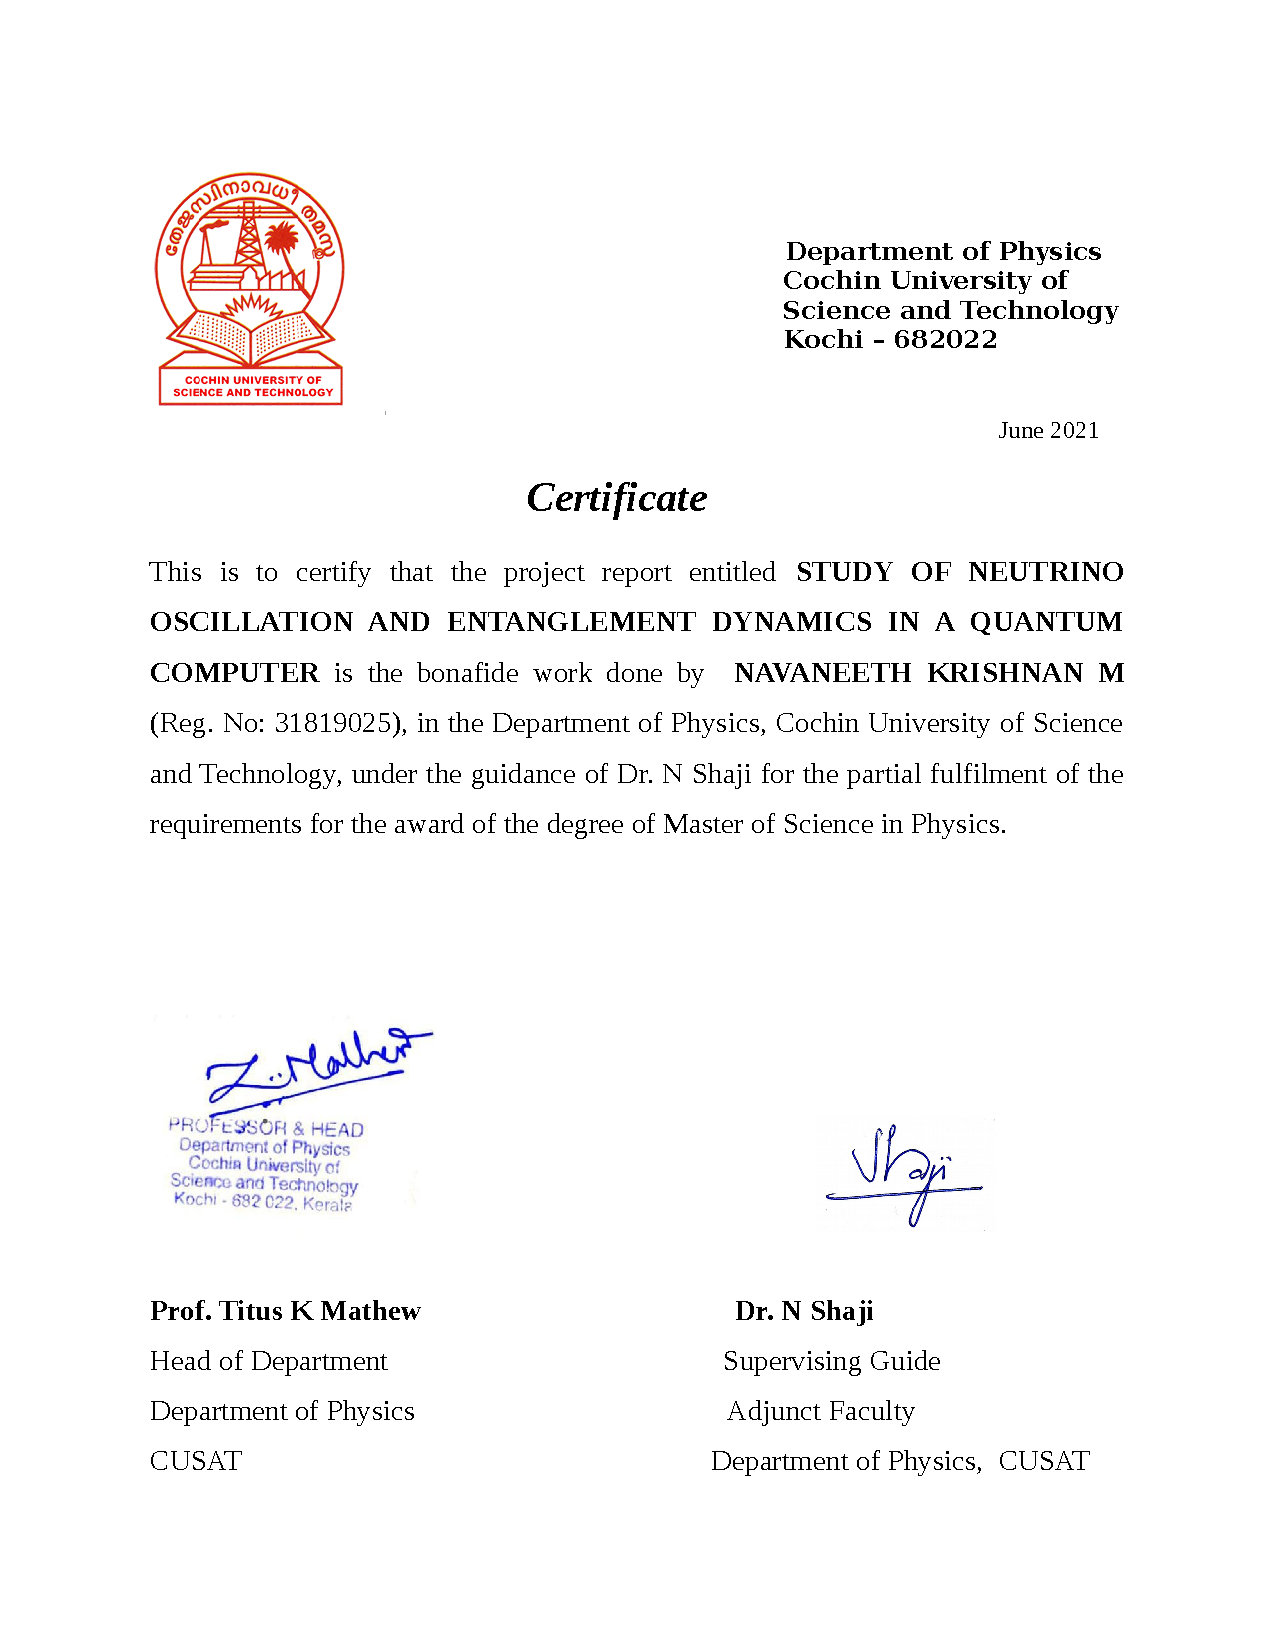
\includepdf[pages=-]{navaneeth.pdf}
\begin{comment}
\begin{minipage}{0.2\textwidth}
	\begin{flushleft}
		\graphicspath{ {./Images/} }
		
\includegraphics[width=3cm]{cusat.png}\\[0.5\baselineskip]
	\end{flushleft}
\end{minipage}
\begin{minipage}{0.75\textwidth}
	\begin{flushright}
		{\bfseries
			Department of Physics\\
			Cochin University of Science\\
			and Technology\\
			Kochi -- 682022}
	\end{flushright}
\end{minipage}
\begin{center}
	\hrulefill \\ [1.0cm]
	\begin{flushright}
		\date{10-06-2021}
	\end{flushright}
	\vspace{8mm}
	\emph{\LARGE\textbf{ Certificate}}\\[1.5cm]
	
\end{center}
This is to certify that the project report entitled \emph{\bf Study of Neutrino Oscillations and Entanglemet Dynamics in a Quantum Computer} is a bonafide work done by {\bf Navaneeth Krishnan M} (Reg. No. : 31819025), in the Theory Divison, Department of Physics, Cochin University of Science and Technology, under the guidance of Dr N Shaji for the partial fulfilment of the requirements for the award of the degree of Master of Science in Physics.

\vspace*{2.7cm}

\noindent\textbf{Prof. Titus K Mathew} \hfill \textbf{Dr N Shaji} \\
Professor and Head\hfill Project supervisor\\
Department of Physics \hfill  Adjunct Faculty\\
 CUSAT  \hfill Department of Physics,
 CUSAT\\
 \end{comment}
 \newpage
\thispagestyle{empty}
\vspace{2cm}
\begin{center}
	\vspace{2cm}
	\emph{\LARGE\textbf{Declaration}}\\[1.8cm]
\end{center} 
I hereby declare that the thesis entitled ``\textbf{Study of Neutrino Oscillations and Entanglemet Dynamics in a Quantum Computer}" is the work done by me under the guidance of \textbf{Dr N Shaji}, Adjunct Faculty, Department of Physics, Cochin University of Science and Technology.

\vspace{2.5cm}
\noindent{Cochin - 682022 \hfill Navaneeth Krishnan M}\\
\noindent{14-06-2021}
\begin{center}
	\chapter*{Acknowledgements}
\end{center}
\addcontentsline{toc}{chapter}{\numberline{}Acknowledgements}

With great pleasure, I express my sincere gratitude to Dr N Shaji, Adjunct Faculty, Department of Physics, Cochin University of Science and Technology, my supervising guide, for all his advice, encouraging words and patience. I am thankful to Prof. Titus K Mathew, Head of the Department of Physics, Cochin University of Science and Technology, for providing the necessary facilities to carry out this work. I want to thank Mr Manosh T. M (Research Scholar) and Dr Dintomon Joy for their immense help and encouragement. This project is the fruit of their unwavering patience and guidance. I also express my sincere gratitude to my friend Ms Shilpa Prakash for the time she spent discussing concepts with me. I also thank all the teachers, research scholars, staff and all my friends of the Department of Physics, CUSAT.  Most importantly, I would like to thank my parents and my sister. They continually stand beside me and encourages me in every step I take.\\ 

\hfill \textbf{Navaneeth Krishnan M}

\chapter*{Abstract}\vspace{-3em}
\addcontentsline{toc}{chapter}{\numberline{}Abstract}
Classical simulations became a part of a researcher's toolkit during the second world war. In the late 1940s, Stanislaw Ulam introduced Monte Carlo simulations to simulate nuclear detonation. After that, many algorithms to simulate both classical and quantum systems were put forward. However, soon we understood that a classical system like an ordinary computer is ill-equipped to simulate the complex quantum system. It led to the notion of Quantum Simulations, where we use simpler and controllable quantum systems to simulate the complex ones. The main hurdle in quantum simulation is finding a mapping scheme that map one system on another. It often involves some assumptions but does not suffer from an exponential explosion in the resources required as the classical simulations do. This approach's usefulness is far-reaching and has found its way to Condensed Matter Physics, Cosmology, Nuclear Physics, and Quantum Chemistry. \par
Digital Quantum Simulation uses a quantum computer as the simulator. An ideal quantum computer can simulate any quantum systems that evolve according to the local interactions. This thesis uses digital quantum simulations to study a peculiar behaviour of neutrino known as neutrino flavour oscillation (neutrino oscillation). It is one of the well-studied problems that has given us many insights into particle physics and forces us to look beyond the standard model. We study neutrino oscillation by simulating the time evolution of the neutrino using a quantum circuit (quantum algorithm) put forward by Arguelles and Jones in 2019. We report oscillation probabilities (the probability of neutrino undergoing falvour oscillation) as a function of time that matches with the theoretical predictions. Our study also confirms that neutrino oscillations greatly influence the neutrino's entanglement. We conduct the study on the entanglement dynamics of the system by quantifying entanglement using entanglement entropy. We use linear entropy of the neutrino as a measure which we directly calculate through quantum simulation of the system. Our analysis of how the linear entropy changes with time enabled us to show how entanglement changes with time, revealing its dynamical nature.


\newpage
\pagebreak	
{
	\hypersetup{linkcolor=black}
	\tableofcontents
	\listoffigures
}
\chapter*{Introduction}
\addcontentsline{toc}{chapter}{\numberline{}Introduction}
\emph{“Can physics be simulated by a universal computer? [...] the physical world is quantum mechanical, and therefore the proper problem is the simulation of quantum physics [...] the full description of quantum mechanics for a large a system with R particles [...] has too many variables, it cannot be simulated with a normal computer with a number of elements proportional to R [ ... but it can be simulated with ] quantum computer elements. [...] Can a quantum system be probabilisticaly simulated by a classical (probabilistic, I’d assume) universal computer? [...] If you take the computer to be the classical kind I’ve described so far [..] the answer is certainly, No!"} 
\begin{flushright}
- Richard P Feynman \cite{feynman82}\cite{nielsen}
\end{flushright}

Solving differential equations, which encapsulate the physical principles guiding the dynamical behaviour of a system, lies at the heart of many simulations. One of the most simple example of such an equation is the Newton's equation of motion,
\begin{equation}
m\frac{d^{2}x}{dx} = F
\end{equation}
Generally, the initial state of the system would be input to the problem. Using simulations, one aims to predict the state of the system at a later time or position. The first step in doing any simulation is the encoding of state of system digitally, which more often involves some approximation. Using the encoding scheme, we have to prepare the initial state of system. Then one has to discretize the dynamical differential equation in space and time. Discretization should be done in such a way that the iterative application of a procedure should evolve the state from initial to final conditions. The accuracy of output state predicted by the simulator depends upon discretization length. Theoretically, as the length of discretization decreases the result would be more accurate. But while computing we need to consider other errors that can arise while decreasing the discretization length. Thus often an optimum value of discretization length would be better. Now, why this approach works?. This works because the error is bounded and does not considerably grows as the number of iterations increases. Further, only those system that can be efficiently described can be simulated efficiently. Thus, there are systems where such an approach fails.\par
Now comes the question of whether we can simulate a quantum system using a classical simulator. The short answer is yes. But it should be noted that often such simulations are inefficient and fail when the number of particles in the system is very high.  When we analyse the problem of simulating a quantum system, for most of simple quantum systems, the evolution is governed by the Schrodinger equation. 
\begin{equation}
i\hbar \frac{d}{dt}\ket{\psi} = \hat{H} \ket{\psi}
\end{equation}
On the position basis, the above equation will be 
\begin{equation}
i\hbar\frac{\partial}{\partial t}\psi(x)= \left[ -\frac{\hbar^{2}}{2m}\frac{\partial^{2}}{\partial x^{2}}+V(x)\right] \psi(x)
\end{equation}
Where $\braket{x|\psi} = \psi(x)$.\par
Assume that we wish to simulate a simple two-level system (qubit) that obeys Schrodinger equation. For such as system, we have to solve two differential equation to simulate it. If it is a two-qubit system then there would be four equations and so on. Thus, a general system of n qubits $2^{n}$ differential equations must be solved to simulate it. This exponential explosion in the equation is unavoidable unless we employ some approximate methods like Monte Carlo methods \cite{monte} which considerably reduce the number of equations. Such classical stochastic methods would allow us to evaluate the phase-space integrals of many-body quantum systems in polynomial time. But these methods are efficient while the function being integrated does not change its sign. Thus while using such methods, sampling of the function is done in a relatively small number of points. For systems like fermionic or frustrated systems, the integrals encounter the problem of sampling with non-positive semi-definite functions (referred to as negative sign problem \cite{troyer}\cite{georgescu}) which cause an exponential increase in computation time as the number of particles increases. Thus in such systems, Monte Carlo methods are shown to be inefficient. Other than Monte Carlo methods, there are methods like Density Functional Theory (DFT) \cite{dft}, mean-field theories, Green function-based methods, many-body perturbation theories \cite{mbpt} etc. These methods also have there own limitations.

Richard P Feynman was one of the persons who put forward a solution to this problem. He said that \emph{“Let the computer itself be built of quantum mechanical elements which obeys quantum mechanical laws"} \cite{feynman82}. Feynman realized that such a quantum system - which later called a quantum computer - would be able to handle the exponential explosion of parameters that happen while solving a large number of equations without using an exponentially large number of physical resources. Even though Feynman proposed such a radical idea, he was not sure of how to realise simulations in such controllable quantum systems. More than a decade later, it was Lloyd who showed that quantum computer could act as a universal quantum simulator \cite{lloyd}. Here the term “universal” is used in the sense that the same system can be used to simulate vastly different problems. Of course, one has to make adjustments in the algorithm according to problem. 

Even though the quantum computer was proposed to simulate quantum systems, its uses extend far beyond it. The past three decades have revealed the true potential of a quantum computer. Nowadays quantum computing and quantum information itself a topic of research. Further, it became later clear that we don’t always need a quantum computer for implementing quantum simulations. For simulating a particular quantum system, we only need a simple quantum system that has similar time evolution. That is, simple quantum devices that mimic the time evolution of other quantum systems can be used as simulators. But the drawback of such an approach is that such a simulator would be problem-specific (not universal). On the bright side, such simple systems can be easily controlled and designed compared to sophisticated quantum computers.

Based on the approach, we can broadly classify the quantum simulations into two kinds; Analog Quantum Simulation (AQS) and Digital Quantum Simulations (DQS). In DQS we use quantum computers as simulators. Here we encode the time evolution of the quantum system in a quantum circuit comprising qubits and quantum gates.  The circuit is designed in such a way that the output of the circuit gives the time evolved state of the system under study.  A similar but different approach is taken in Analog Quantum Simulations. In AQS, a simple quantum system that is controllable is created depending upon the problem. This system is designed in such a way that it would mimic the time evolution of the system under study. Thus in this approach, simulations are done using a simple quantum system as simulators.

In recent years, the field of quantum simulations has gained momentum. The sudden spike in interest is two-fold. The first one is its wide range of application. For instance, quantum simulations can be used in condensed matter for studying many difficult problems like quantum phase transitions, high Tc superconductivity, quantum magnetism etc. Other potential applications include fields like high energy physics, nuclear physics, cosmology, quantum chemistry etc. The second factor that accelerated the growth of quantum simulations is the recent progress in the field of quantum technologies. Recent years have witnessed development in different types of realization of quantum computers. Nowadays quantum computers are publicly accessible. %Quantum simulators which can be used to perform simulations repeatedly are now available.
Technologies to maintain coherent control over the system and to perform measurements have matured enough to make simulations possible. But still have a long way to go for the efficient simulation of quantum systems.

In near future, quantum simulations will become a prominent tool for research in a wide variety of fields. In this milieu, the study of quantum simulations holds importance. This was the motivation for us to conduct this study. Here we are interested in the digital quantum simulations of phenomena called Neutrino oscillation. We use the quantum computing services provided by IBM to carry out our simulations. The scheme for such a simulation was put forward by Arg\"uelles and Jones in 2017 \cite{jones}. They have encoded neutrino oscillation into a quantum circuit. Time evolution of the qubits is done by applying unitary single and two-qubit gates. The exact scheme will be discussed in the following sections $\ref{sec4}$ and $\ref{sec5}$. 

In nature, neutrinos are produced in three distinct flavours electron, muon and tau. Neutrinos are produced through weak interactions. As a neutrino beam propagates from source to detector neutrino flavour oscillate between the three flavours. The first evidence of neutrino flavour oscillation came from the famous Ray Davis Homestake experiment \cite{ray}.  He reported a deficit in the flux of solar neutrinos (electron neutrinos)  from the value predicted by the Standard Model. He used a chlorine-based detector and obtained a flux that was three times less than that of the theoretical value.  This observation of Ray Davis later came to be known “Solar Neutrino Problem”. For his contributions in the field of astrophysics, Ray Davis was awarded the Nobel prize in Physics in 2002. 

Following the Homestake experiment, different sorts of powerful detectors were set up to study the problem. All the experiments confirmed the deficit of neutrinos in the solar flux. Ray Davis performed his experiment in the 1960s. Interestingly, the idea of neutrino oscillation was put forward by Pontecorvo in 1957 \cite{ponte57}. Thus one can say that solution existed even before the problem. But in Pontecorvo’s version, neutrino-antineutrino undergo oscillation. He put forward this theory in analogy with the neutral kaon mixing that was known way before. Although such oscillations do not occur in nature, this formed a key conceptual foundation in developing the theory for neutrino oscillation. The theory for neutrino flavour oscillation was put forward first by Maki, Nakagawa, Sakata in 1962 \cite{maki} which was later elaborated by Pontecorvo in 1967 \cite{ponte68}. The solar neutrino deficit observed only a year after that. The solar neutrino problem baffled scientists for a long time. It was the team of Canadian scientists lead by Arthur B McDonald in Sudurbary Neutrino Observatory (SNO) that put an end to the mystery. They experimentally verified that electron neutrino produced in the sun undergo flavour oscillations. The deficit in the number of electron neutrinos was because neutrinos undergo flavour change while travelling to Earth \cite{mcdonald}. At the same time, a group of Japanese scientist led by Takaaki Kajita verified neutrino oscillation by studying atmospheric neutrinos. Atmospheric neutrinos were produced when cosmic rays hit the Earth’s atmosphere. When it travels to the Earths surface they undergo flavour oscillations. The team led by Kajita was able to detect these flavour oscillations. For the experimental verification of neutrino flavour oscillation, both Kaajita and McDonald was awarded the Nobel prize in physics in 2015.

The verification that neutrinos can undergo oscillations comes with great consequences. It was known that neutrinos can undergo flavour oscillation only if they have mass. But according to the Standard Model, neutrinos are massless. Thus the phenomenon of neutrino oscillation insists on the modification of the standard model. Even though there are some minimal extensions of the Standard model to accomodate neutrino masses, exact theory is still unknown.  Neutrino oscillation experiments gives us mass squared splittings and mixing angles. This will be discussed later. But till now the actual mass of the three neutrinos are still unknown. Thus the study of neutrino oscillation is a door to explore physics outside the standard model. 

In this work, we performed simulation of the time evolution of a neutrino flavour state. During such simulations we were able to observe neutrino flavour oscillations. But the application of DQS extends more than the temporal evolution of the state of the system. DQS can be used to obtain certain properties of a quantum system. It has been shown that using DQS we can estimate the eigenvalues of the operators including Hamiltonian of the system. For example, Abrams and Lloyd have put forward an algorithm to find eigenvalues and eigenvectors of Hamiltonian \cite{abrams}. They have proposed an algorithm that uses quantum fast Fourier transform to evaluate eigenvalues and eigenstates. Similarly, Aspuru-Guzik \emph{et al.} by applying a recursive phase estimation algorithm have calculated the molecular ground state energies of lithium hydride and water molecule \cite{aspuru}. It has been also shown that DQS can be used to compute the partition function of the system \cite{lidar}. Moreover, people have shown that classical physics can efficiently be simulated by quantum computers \cite{meyer}\cite{sinha}. 

Here we used the DQS of neutrino oscillation to study the entanglement between different neutrino flavours. Blasone \emph{et al.} through a series of papers \cite{blasone2008}\cite{blasone2009}\cite{blasone2010}\cite{blasone2014}, have proposed the existence of single particle entanglement in neutrinos. It was van Enk who proposed single particles can have entanglement \cite{vanenk2003}\cite{vanenk2005}\cite{vanenk2006}. He explained single particle entanglement in the context of single photons. Blasone \emph{et al.} extended these concepts into the case of neutrinos. They also provided scheme to quantify the degree of entanglement in the system. They used a measure called \emph{entanglement entropy} to quantify the entanglement. We applied their results in to our circuit and were able to accurately predict the entanglement dynamics of the system. 

This report is organized as follow. In the first chapter [\ref{sec1}], we provide a brief introduction to quantum simulations. Different types of approach for performing quantum simulations are discussed in this chapter. The second chapter [$\ref{sec2}$] is dedicated for the discussion of neutrino oscillation. In this section, we discuss the neutrino oscillation theory (both two flavour and three flavour case) relevant for performing quantum simulations. In the following chapter [$\ref{sec3}$], we discuss about the entanglement in the neutrino. Chapter [$\ref{sec4}$] and Chapter [$\ref{sec5}$] deal with the simulation of neutrino in a quantum computer. The scheme of performing such a simulation is given in the fifth chapter. The following chapter contains the results of the simulations performed. The conclusions and outlook is given in the concluding section.


\newpage
\thispagestyle{empty}
\mbox{}
\newpage
\chapter{Quantum Simulations: An Overview}\label{sec1}

Simulating a quantum system by quantum mechanical means is defined as quantum simulation. For performing simulations, we need a quantum simulator.  By definition, a quantum simulator is a controllable quantum system that can simulate or mimic other quantum systems. As discussed earlier, based on the type simulator used we can classify simulations as Digital and Analog quantum simulations. There is one more type of simulation method that belongs to the class of quantum simulations. It is called “Quantum Information inspired algorithms for classical simulations of quantum systems”. We will briefly discuss all of them in the following sections. Before that, we provide a bit more explanation on the advantage of quantum simulation over classical simulation.

As we have discussed in the introduction, simulating a system often include three steps: preparation of the initial state, time evolution of the state and measurement of the final state. Let the system we want to simulate be a system of $N$ spin-half particles. The system is described by state vector $\ket{\psi}$ at some time $t$. We have to encode the state first into the simulator.  If we perform classical simulation, to encode $\ket{\psi}$ we need to store $2^{N}$ numbers in memory. The $2^{N}$ numbers represents the complex probability amplitudes of different spin configuration. Here we implicitly assume that spins do not have motional degrees of freedom. Now to get a physical sense of the problem, let us fix the value $N=40$. Then we have to store $2^{40} \approx 10^{12}$ numbers for encoding $\ket{\psi}$. If we assume single-precision (7 decimal digits of precision), we would approximately need $\sim 3 \times 10^{13}$ bits. In terms of memory, it would correspond to $4$TB (terabytes) memory \cite{lloyd}\cite{georgescu}. If we double the number of spins it would require $\sim 3 \times 10^{25}$ bits (or $5 \times 10^{12}$ TB). Now, while using a quantum computer, we only need $N$ qubits to represent $N$ spins. Thus a system of $40$ spins can be represented by a $40$-qubit ($5$ quantum byte) register. Further, the quantum computer provides exponential compression of the memory space required. Recently, a research group have shown that it only takes $\log_{2} [N+1]$ qubits to store $N$ identical qubits \cite{rozema}. That is, it only takes $10$-qubit memory to store $1000$ identical qubits and $11$-qubit memory for $2000$ qubits and so on. It is evident that in classical simulations, an exponential number of resources are needed. This is usually referred as \emph{exponential explosion}.

Now for doing simulations, if we consider the most general case, we have to apply an arbitrary unitary transformation to the initial state. This unitary transformation matrix would be realised by logical gates in classical computation and would be replaced by quantum gates in quantum computation. Interestingly, as noted by Lloyd \cite{lloyd}, the number of quantum gates required to an arbitrary unitary transformation is of the same order as logical gates required in classical computation. Thus, at first glance, one would be sceptical about the quantum advantage. But it should be noted that there is a small difference between what we said and what Feynman proposed. Feynman conjectured that systems that evolve according to local interactions can be efficiently simulated by a quantum computer. That is, for quantum simulation to be efficient, system should undergo non arbitrary unitary transformation.  We are particularly interested in the time evolution of the system. Such a transformation is not arbitrary in nature. In general, any system that is consistent with Special and General Relativity evolves according to the local interactions \cite{lloyd}. Hamiltonian of such a system will be of the form,
\begin{equation}
H= \sum_{l=1}^{M} H_{l}
\end{equation}
Where $H_{l}$ represents local interaction Hamiltonian. For such type of systems, Lloyd has shown quantum simulations are more efficient than classical simulations \cite{lloyd}.

The next obvious step of a simulation is the measurement of the final state. While doing the simulation using a classical computer it is not a big task. Technology has developed so much and we can considerably reduce readout errors in classical computers. But when it comes to a quantum computer, measurement isn’t a walk in the park. Measurement is the only non-unitary transformation that we apply to the qubit.  Direct measurement of the state of the qubit destroys its quantum nature.  Also during measurement, due to interaction with outside, decoherence can happen to the qubit. Decoherence would induce errors in our measurement result. To prevent this we usually perform non-demolition measurements that would not alter the state of the qubit. In such sort of measurements simulators have less interaction with their surroundings. Thus quantum information would be preserved and qubits would remain coherent. 

The decoherence and thermal effects affecting the simulator can be exploited to mimic decoherence effects of the system we study. This feature sets apart quantum simulation from its classical counterpart. Thus, in short, in instances we have to simulate a quantum system, quantum simulations outperform classical simulations. Quantum simulation prevents the exponential explosion. This is inevitable in classical simulation as the number of quantum variables increases. With that said, we are now going to discuss different types of quantum simulations.
\section{Digital Quantum Simulations (DQS)}
Circuit (quantum circuit) based simulation  of a quantum system is called Digital Quantum Simulation. In this approach, we create a quantum circuit using qubits and quantum gates that mimic the time evolution of the system. For building such circuits, we first have to encode the state vector $\ket{\psi}$ in the computational basis. If we take the example of a system of N spins, it can be encoded using the scheme,
\begin{gather*}
\ket{\uparrow} \rightarrow \ket{1} \ ; \ \ket{\downarrow} \rightarrow \ket{0}
\end{gather*}
Using the encoding scheme, we need to initialize the state of the system in the quantum register. This is called initial state preparation. It should be noted that encoding scheme may vary from one system to other. In many cases, initial state preparation is not an easy task. Efficient algorithms initializing the state often will not be available. %But there are cases where the initial state can be prepared easily.
 
To get state of the system at time $t$, we have to apply the time evolution operation $\exp\left(-i\frac{Ht}{\hbar}\right)$ to initial state $\ket{\psi (0)}$. The time evolution operator is unitary. In principle, any unitary operation can be represented by using quantum gates. Thus is DQS, time evolution operation is realised using quantum gates. During simulation, we apply a time-ordered sequence of gates to the initial state created.

Now, finding an efficient decomposition of Hamiltonian in quantum gate basis is itself a difficult problem. Most of the time evolution we implement would be an approximation of actual evolution. Also as Feynman pointed out, not all systems can be simulated. DQS can only be applied to a system whose Hamiltonian can be written as sum of many local interactions. Form of such a Hamiltonian is given by equation,
\begin{equation}
H= \sum_{l=1}^{M} H_{l}
\end{equation}
Examples of such systems include the Hubbard model, Ising model etc.

If $[ H_{l}, H_{l’}] =0$ for all $l$ and $l’$, then time evolution operator will be,
\begin{equation}
U = \prod_{l} e^{-i\frac{H_{l} t}{\hbar}} 
\end{equation}
In such cases, the decomposition in terms of gates is straight forward can be easily done. Unfortunately for most of the cases of physical interest $[ H_{l}, H_{l’}] \neq 0 $. 
Then we have to resort to approximate methods for decomposition. In such cases, We discretize the evolution time into a large number of steps. Each step is of duration $\Delta t$. Then U can be written as,
\begin{equation}
U = \left[e^{-i\frac{H\Delta t}{\hbar}}\right]^{\frac{t}{\Delta t}}
\end{equation}
Using approximate methods like the first order Trotter formula we can decompose $\exp\left(-i\frac{H\Delta t}{\hbar}\right)$ into quantum gates. 
\begin{equation}
U(\Delta t) = e^{-i\frac{\sum_{l} H_{l}\Delta t}{\hbar}} = \prod_{l} e^{-i\frac{H_{l}\Delta t}{\hbar}}+ \mathcal{O}(\Delta t^{2})
\end{equation}
As a result when $\Delta t \rightarrow 0$ i.e. steps of infinitesimal duration
\begin{equation}
U(\Delta t) \approx \prod_{l} e^{-i\frac{H_{l}\Delta t}{\hbar}}
\end{equation}
Now, to have high accuracy, $\Delta t$ should be very small which in turn increases the number of gates. But in the quantum computers now available, the error increases with the number of gates applied. So in a practical scenario, we can only approximately decompose $\exp\left(-i\frac{H\Delta t}{\hbar}\right)$. Further, there are results that emphasising the shortcomings of first-order trotterization \cite{brown}\cite{clark}.  They have shown that decomposition can be more efficient by including higher order terms. Discussions about such methods can be found in \cite{nielsen}. 

After time evolution, we have to get back the output state from the circuit. In general, to completely reconstruct the state, we use a technique called Quantum State Tomography (QST).  In QST, we make many identical copies of the system. Then we perform a series of measurement along with different bases. To have a minimalistic understanding of how this method works, it useful to consider the parable “Blind men and an elephant”. In the parable, five blind men describe a different aspect of the elephant. Combining all of their observation would give the whole picture of an elephant. Similarly, a series of measurements on identical copies of the state, each allows a glimpse into a distinct aspect of a quantum state’s reality. Each new measurement illuminates a different dimension of an unknown state. But while this method, the resources required would grow exponentially with the size of the system. So in most cases, projective measurements are done at the end of the circuit. In this sort of measurement, the state of the system is projected to a computational basis while measuring. 

\section{Analog Quantum Simulations (AQS)}
Simulation of a quantum system using another quantum system that mimics the time evolution of the former is called Analog Quantum Simulations. A general scheme for AQS is given in the figure.\par
\begin{figure}[h]
\graphicspath{ {./Images/} }	
{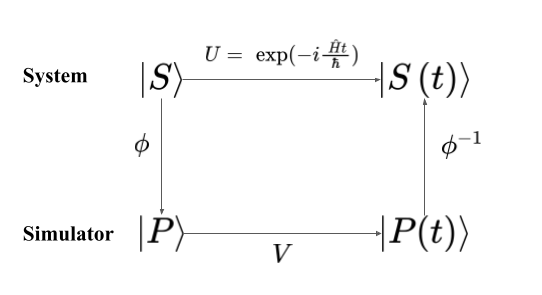
\includegraphics[width=0.8\textwidth]{fig_10.png}}
\centering
\caption{Scheme for analog simulations}
\label{fig 10}
\end{figure}
$\ket{S}$ and $\ket{S(t)}$ represent the initial and final state (time evolved state) of system. Similarly, $\ket{P}$ and $\ket{P(t)}$ represent initial and final state of the simulator. 
Here the system is mapped to the simulator via an invertible map $\phi$ (unitary operator). This mapping determines the correspondence between the states and operators of the system and simulator.\par
If we follow such a scheme described by figure $\ref{fig 10}$, the evolution operator $U$ and $ V$ would be connected by,
\begin{equation}
V = \phi U \phi^{-1}
\end{equation}
If mapping is unitary, we can write,
\begin{equation}
V = e^{- i\frac{H_{sim} t}{\hbar}}
\end{equation}
Where $H_{sim} = \phi H_{sys} \phi^{-1}$.\par
Thus while simulation we map the initial state $\ket{S}$ to $\ket{P}$
\begin{equation}
\ket{P} = \phi \ket{S} 
\end{equation}
Then simulator is allowed to time evolve $\ket{P} \xrightarrow{V} \ket{S}$. After time evolution final state $\ket{P(t)}$ is mapped back to $\ket{S(t)}$.
\begin{equation}
\ket{P(t)} = \phi^{-1}\ket{S(t)}
\end{equation}
Thus eventually we get back the time evolution of the system $\ket{S} \rightarrow \ket{S(t)}$.

Now we are going to discuss a very simple scheme of mapping between quantum system and simulator. The scheme we are discussing was proposed by Somaroo \emph{et al.} (1999)\cite{somaroo} for simulating a quantum harmonic oscillator on two proton nuclear spins in 2,3-dibromothiophene. Note that here the number of states available for QHO is restricted to four. The convenient unitary mapping of system and simulator is,
\begin{gather*}
\ket{n=0} \leftrightarrow \ket{\uparrow\uparrow}
\ket{n=1} \leftrightarrow \ket{\uparrow\downarrow}
\ket{n=2} \leftrightarrow \ket{\downarrow\uparrow}
\ket{n=3} \leftrightarrow \ket{\downarrow\downarrow}
\end{gather*}
One doesn’t need to have followed this mapping. The mapping presented above is simple and straight forward. \par
The time evolution operator of QHO is given by
\begin{equation}
U = e^{-i\frac{H_{\tiny QHO} t}{\hbar}} \equiv \exp\left[-i \frac{\left(\frac{1}{2}\ket{0}\bra{0} + \frac{3}{2}\ket{1}\bra{1} + \frac{5}{2}\ket{2}\bra{2} + \frac{7}{2}\ket{3}\bra{3}\right)\omega t}{\hbar}\right]
\end{equation}
Where $\omega$ is the oscillatory frequency. From this, we can find the time evolution of the simulator.
\begin{equation}
\label{eq:19}
V = e^{-i\frac{H_{sim} t}{\hbar}} \equiv \exp\left[-i\frac{\left(\frac{1}{2}\ket{\uparrow\uparrow}\bra{\uparrow\uparrow} + \frac{3}{2}\ket{\uparrow\downarrow}\bra{\uparrow\downarrow} + \frac{5}{2}\ket{\downarrow\uparrow}\bra{\downarrow\uparrow} + \frac{7}{2}\ket{\downarrow\downarrow}\bra{\downarrow\downarrow}\right)\omega t}{\hbar}\right]
\end{equation}
In Pauli basis ${\sigma_{x},\sigma_{y},\sigma_{z},I}$, equation $\ref{eq:19}$ can be rewritten as ,
\begin{equation}
\label{eq:20}
V = exp\left[i\left(\sigma_{z}^{2}(1 + \frac{1}{2}\sigma_{z}^{2}) - 2 \right)\omega t\right]
\end{equation} 
Thus the simulator evolves according to equation $\ref{eq:20}$. At the end of the simulation, final state of the simulator is measured. The resultant state is mapped back into the QHO state.\par

Sometimes we will not to be able to simulate the entire system. But mapping can be done in such a way that it could be used to study some characteristic of the system. In general, the mapping we use depends upon the characteristic of the system we intend to study and the properties of the simulator. In AQS the physical quantities can be measured directly from the simulator. Since it is analogous to the system, measurement results yield information about the system. This is an added advantage since in DQS we need to computationally manipulate the measurement results. Also in AQS even if there are some error we can use it to perform qualitative studies. For example, we can use it to investigate properties like phase transition. But the error rate should be below a tolerance level.

Now in the example, we have shown, the mapping was simple and straight forward. But generally, this is not the case. Sometimes clever mapping schemes have to formulated to efficiently simulate a system. Further discussion in this direction can be seen in the reference \cite{georgescu}.

\section{ Quantum-Information-Inspired Algorithms for Classical Simulation of Quantum Systems }
In this mode of approach, classical algorithms are used in the simulation of the quantum many body systems. But as discussed before, normal classical algorithms are prone to exponential explosion. Here in order to prevent this and to efficiently perform simulations we seek the assist of quantum information theory. First approach in this direction was done by Verstraete \emph{et al.}(2004), they analysed the Density Matrix Re-normalization Method from a quantum information perspective \cite{cirac}.\par This new hybrid class of algorithms help in efficient simulations of quantum lattice systems. Moreover, these methods can be combined with Monto Carlo Techniques to improve its efficiency. For example, it has been shown the quantum version of Metropolis alogarithm overcomes the sign problem that we discussed before \cite{temme2011}.
\newpage
\thispagestyle{empty}
\mbox{}
\newpage


\chapter{Neutrino Oscillation}\label{sec2}

A neutrino  ($\nu$) is a an elementary particle with a spin of $\frac{1}{2}$. It undergoes interaction only via the weak interaction and gravity. It was Pauli who proposed the idea of neutrino. According to him, neutrino is a non-interacting, neutral particle. He proposed the existence of such a particle to recover conservation laws in the case of beta decay. At that time beta decay was appearing to violate energy, momentum, and angular momentum conservation laws. Even though they are abundant on universe since they undergo only weak interaction, they rarely interact with matter and thus are incredibly difficult to detect. Therefore first detection of neutrino only occurred $25$ years after it was first proposed. First detection of neutrinos was made by two American physicists Clyde Cowan and Frederick Reines. The detected anti neutrinos which were emitted by a nuclear reactor. For this discovery Frederick Reines was awarded the Nobel Prize in Physics in $1995$. \par

During weak interactions neutrinos are created along with a corresponding charged lepton. The flavour of neutrino produced depends upon the lepton produced. They were proposed to be a massless particle.  But it was later found that neutrinos do have mass. But till now we are not able to measure accurate mass of a neutrino. This is because the flavour state of neutrino doesnot coincide with its mass states. In other words, neutrinos have three discrete masses but they do not correspond to three flavours. A neutrino flavour state can be considered as quantum superposition of all mass states or mass eigenstates. \par

During an experiment neutrinos produced via weak interaction are sent to detector placed at a distance. Neutrinos are emitted and absorbed as flavour states but travel as mass eigenstates. During the flight, three mass states will accumulate a quantum mechanical phase. The phase accumulated depends upon the mass of the state (will discuss it later). When neutrinos reach detector, these mass states interfere producing a neutrino of particular flavour. The neutrino produced at the detector need not be of the same flavour as that at the source. For fixed value of neutrino beam energy, flavour state detected varies as a function of distance. That is, flavour of neutrino at the detector depends only on the distance between source and detector. This is phenomenon is called Neutrino oscillations.\par

As said before, a particular flavour state is a superposition of mass states. Each mass state is characterised by a definite mass. If we take plane wave solutions for mass state, the phase accumulated by the mass state depends upon its mass (will be shown later). Then neutrino oscillation can be studied as interference of mass eigenstates. Thus the probability of detecting a particular flavour in a particular distance depends upon difference in the phase. These phase difference vary as function of distance and energy of the neutrino beam. This will be shown later. As a result of this, as neutrinos travel, it will be the admixture of all three flavours. The probability of detecting a flavour can be found out. It is found to be depend in sinuosoidal manner on the source-detector distance and energy of the beam. Square of mass differences between neutrino flavours are small of $\mathcal{O}({10^{-5}})eV^{2}$ . The coherence length will be very high compared to mass differences. Thus this microscopic quantum effect becomes observable over macroscopic distances.\par

Over a decade of research, physicists Pontecorvo, Maki, Nakagawa, and Sakata developed the theory of neutrino oscillation. They found that in an ultra-relativistic scenario, the composition of the flavour state is given the PMNS matrix. But in $1985$ Mikheyev and Smirnov modified the theory of neutrino oscillation to include matter effects on neutrino oscillation. Initial work in this direction was done by Wolfenstein in $1978$. This effect is thus called Mikheyev Smirnov Wolfenstein effect (MSW effect). 

\section{Neutrino Flavour Oscillation in Vacuum}\label{FO}
A neutrino source produces a neutrino along with a charged lepton. Flavour of the lepton ($e,\mu$,or $\tau$) produced would give us the flavour of neutrino produced ($\nu_{e},\nu_{\mu}$,or $\nu_{\tau}$). A neutrino created in a specific flavour eigenstate would be superposition of all three mass eigenstates. The relationship between flavour and mass states is encoded in the PMNS (Pontecorvo-Maki-Nakagawa-Sakata) matrix. It is a unitary mixing matrix that contains information on the mismatch of quantum states of neutrinos when they propagate freely and when they take part in the weak interactions. Experiments have established values for the elements of this matrix \cite{zyla}.\par
Experimentally, a neutrino beam of known flux and flavour $\alpha$ is produced along with lepton $l_{\alpha}$ at the source. It is the lepton formed that gives us the flavour of neutrino produced. Neutrino is then send to a detector placed at a distance $L$ from the source. There it would interact with the detector material to produce a secondary lepton $l_{\beta}$ and neutrino $\nu_{\beta}$.  Thus at the time of interaction (with detector material), the neutrino would in $\beta$ flavour ($\nu_{\beta}$). One could detect the flavour change in two ways. One way is observe the appearance of neutrinos of new flavour $\beta$ that is different from the original flavour ($\beta\neq\alpha$). Such type of experiments are called `appearance experiments' and would give us the appearance probability. The other way is to look for the known flavour $\nu_{\alpha}$. In that case we measure the amount of flux disappeared compared to the initial beam. Such type of experiments are called `Disappearance experiments' and would give us the disappearance probability or survival probability.

\subsection{Theory of Flavour Oscillations}
In order to explain the phenomenon of oscillations, one has to decompose a flavour eigenstate $\ket{\nu_{\alpha}}$ in the mass eigenstate basis $\ket{\nu_{i}}$. In a simple sense, mass eigenstates are the eigenstates of the Hamiltonian. Flavour states ($\ket{\nu_{e}}$, $\ket{\nu_{\mu}}$, $\ket{\nu_{\tau}}$) are not eigenstates of the Hamiltonian and thus do not have definite energy eigenvalue. A mass eigenstate of type $i$ with momentum $p_{i}$ is an energy eigenstate with eigenvalues  $E_{i}=\sqrt{p_i^{2}+m_{i}^{2}}$ (in natural units). Flavour and mass eigenstates are connected via PMNS Matrix which is unitary. The matrix equation connecting flavour and mass states are given by:
\begin{gather}
 \begin{bmatrix} \ket{\nu_{e}} \\ \ket{\nu_{\mu}} \\ \ket{\nu_{\tau}} \end{bmatrix} = 
 \begin{bmatrix} U_{e1} & U_{e2} & U_{e3} \\ U_{\mu 1} & U_{\mu 2} & U_{\mu 3}\\ U_{\tau 1} & U_{\tau 2} & U_{\tau 3}\end{bmatrix} \begin{bmatrix} \ket{\nu_{1}} \\ \ket{\nu_{2}} \\ \ket{\nu_{3}} \end{bmatrix}
\end{gather}
Thus a flavour state $\alpha$ can be written as a superposition of mass eigenstate.
\begin{equation}
\label{eq:0a}
	\ket{\nu_{\alpha}}=\sum_{i = 1,2,3} U^{\dagger} _{\alpha i}\ket{\nu_{i}}
\end{equation}
Where $\alpha = e,\mu,\tau$  and quantities  may be collected into a matrix known as PMNS matrix or leptonic mixing matrix. According to Standard Model $U$ must be unitary. The relation connecting a particular flavour state to mass eigenstate can be inverted to express a mass eigenstate in terms of flavour state.
\begin{equation}
\label{eq:0b}
\ket{\nu_{i}}=\sum_{\alpha = e,\mu,\tau} U_{\alpha i}\ket{\nu_{\alpha}}
\end{equation}
Where $|U_{\alpha i}|^{2}$ the probability that $\nu_{i}$ interacts with a detector to produce a charged lepton of the flavour of $\alpha$. When standard three flavour oscillation is considered the PMNS matrix is $3\times3$ in nature and for two flavour oscillation, it is $2\times2$. It is given by
\begin{equation}
\label{eq:0c}
U = \begin{bmatrix} C_{12}C_{13} & S_{12}C_{13} & S_{13}e^{-i\delta} \\
S_{12}C_{23}-C_{12}C_{23}S_{13}e^{i\delta} & S_{12}C_{23}-S_{12}S_{23}S_{13}e^{i\delta}& S_{23}C_{13}\\
S_{12}S_{23}-C_{12}C_{23}S_{13}e^{i\delta}& -C_{12}S_{23}-S_{12}C_{23}S_{13}e^{i\delta}&C_{23}C_{13} \end{bmatrix} \begin{bmatrix}
e^{\frac{i\alpha_{1}}{2}}&0&0\\0& e^{\frac{i\alpha_{2}}{2}}&0\\0&0&0\end{bmatrix}
\end{equation}
Where $C_{ij}=\cos\theta_{ij}$, $S_{ij}=\sin\theta_{ij}$. The phase factors $\alpha_{1}$ and $\alpha_{2}$ (Majorana phases) are physically meaningful only if neutrinos are Majorana particles ( i.e. if a neutrino is identical to its antineutrino). Even if present, it does not enter into oscillation phenomena. The phase factor $\delta$ known as the Dirac phase is non-zero only if neutrino oscillation violates CP symmetry, this has not yet have been experimentally observed. So in our discussion for convenience, we take $\delta$ and $\alpha_{i}$ to be zero. In the presence of an additional neutrino, the PMNS matrix gets modified into a $4\times4$ matrix. Such a neutrino is called sterile neutrino. The existence of such a neutrino flavour is not yet confirmed. But there a hints of its existence. Results from Daya Bay reactor experiment and MiniBooNE sheds light on its possible existence \cite{daya}\cite{mini}\par

For simplicity, we first discuss two flavour neutrino oscillation even though all three neutrinos take part in neutrino oscillation. But two neutrino oscillation is a fairly accurate description in a number of experiments. For example, $\nu_{\mu} \rightarrow \nu_{\tau}$ transitions are relevant for atmospheric neutrinos, $\nu_{e}\rightarrow \nu_{\alpha}$ in solar neutrinos, $\nu_{e}\rightarrow\nu_{\mu}$  at reactor experiments and $\nu_{\mu}\rightarrow\nu_{e}$ at accelerator experiments \cite{blasone2009}.\par

Suppose we generate a neutrino beam containing a flavour state $\alpha$. We send the neutrino beam along the x-axis and let them propagate in a free space towards a detector some distance L. Then mass eigenstates propagate according to the time-dependent Schrodinger equation with no potentials.
\begin{equation}
i\frac{d\ket{\nu_{i}(t)}}{dt}=E_{i}\ket{\nu_{i}(t)}
\end{equation}
Here quantities are expressed in natural units ($c=1=\hbar$). Since $L=ct$, in natural units it would become $L=t$. $E_{i}$ is the energy corresponding to the mass eigenstate $\ket{\nu_{i}}$.\par
The solution of this equation is a plane-wave : 
\begin{equation}
\label{eq:0}
\ket{\nu_{i} (t)} = e^{-i\phi_{i}}\ket{\nu_{i} (0)}
\end{equation}
Where $\phi_{i}$ is the phase factor picked up by neutrino during propagation.\par
At some later time $t$ the flavour state $\alpha$ will be : 
\begin{equation}
\label{eq:1}
\ket{\nu_{\alpha}(t)} = \sum_{i=1,2} U_{\alpha i}^{\dagger} e^{-i\phi_{i}}\ket{\nu_{i}(0)}
\end{equation}
Inverting the mixing matrix we can write ;
\begin{equation}
\label{eq:2}
\ket{\nu_{i}(0)} = \sum_{\gamma} U_{\gamma i} \ket{\nu_{\gamma}(0)}
\end{equation}
Substituting equation ($\ref{eq:2}$) in equation ($\ref{eq:1}$), we can write the flavour state as 
\begin{gather*}
\ket{\nu_{\alpha} (t)} =  \sum_{i=1,2} U_{\alpha i}^{\dagger}e^{-i\phi_{i}}
\sum_{\gamma} U_{\gamma i} \ket{\nu_{\gamma}(0)}\\
 = \sum_{i}\sum_{\gamma} U_{\alpha i}^{\dagger} e^{-i\phi_{i}} U_{\gamma i} \ket{\nu_{\gamma}(0)}
\end{gather*}
Thus the amplitude of detecting a neutrino flavour $\beta$ at a spacetime point $(L,t)$ given by,
\begin{equation}
\begin{split}
A(\nu_{\alpha} (0)\rightarrow\nu_{\beta}(t))& = \braket{\nu_{\beta}(t)|\nu_{\alpha}(0)}\\
& =\sum_{\gamma}\sum_{i} U_{\gamma i}e^{i\phi_{i}}U_{\beta i}^{\dagger}\braket{\nu_{\gamma}(0)|{\nu_{\alpha}(0)}}\\
& =\sum_{i}U_{\alpha i}^{\dagger}e^{i\phi_{i}}U_{\beta i}
\end{split}
\end{equation}
Where last step comes from the orthogonality of flavour state $\braket{\nu_{\gamma(0)}|\nu_{\alpha(0)}}=\delta_{\gamma\alpha}$. 
The oscillation probability is given by :
\begin{equation}
\label{eq:3}
\begin{split}
P(\nu_{\alpha} \rightarrow\nu_{\beta})& =|A(\nu_{\beta}(0)\rightarrow\nu_{\alpha}(t))|^{2}\\
&=|\sum_{i}U_{\alpha i}^{\dagger} e^{i\phi_{i}}U_{\beta i}|^{2}\\
&=\sum_{i}\sum_{j}U_{\alpha i} U_{\beta i}^{\dagger} U_{\alpha j }^{\dagger}U_{\beta j}e^{-i(\phi_{j}-\phi_{i})}
\end{split}
\end{equation}

For two flavour oscillation, $U$ would be a $2\times2$ rotation matrix. The rotation matrix would rotate a vector in the flavour basis into a vector in the mass basis and vice versa.
\begin{equation}
U^{\dagger}=\begin{bmatrix}\cos\theta & -\sin\theta \\ \sin\theta & \cos\theta \end{bmatrix}	
\end{equation}
So that,
\begin{equation}
\begin{bmatrix} \ket{\nu_{\alpha}} \\ \ket{\nu_{\beta}} \end{bmatrix} = \begin{bmatrix} \cos\theta & -\sin\theta \\ \sin\theta & \cos\theta \end{bmatrix}\begin{bmatrix} \ket{\nu_{i}} \\ \ket{\nu_{j}}
\end{bmatrix}
\end{equation}
Where $\theta$ is called the mixing angle. It shows how flavour state is different from mass states. If $\theta=0$ the mass states and flavour states exactly coincides. The value of $\theta$ is determined through experiments.\par 
The form of $U$ is substituted in the equation ($\ref{eq:3}$). On reduction, we could arrive at an equation of oscillation probability in terms of mixing angle and $\phi$ as:
\begin{equation}
\label{eq:3a}
P(\nu_{\alpha} \rightarrow \nu_{\beta}) = \sin^{2}\left(2\theta\right)\sin^{2}\left(\frac{\phi_{i}-\phi_{j}}{2}\right)
\end{equation}

In lab frame, since assumed to be plane waves $\phi_{i}$ can be written as ;
\begin{equation}
\phi_{i} = E_{i} t - p_{i}x
\end{equation}

To proceed further, we make an approximation. Usually, we assume the mass eigenstates either created with the same momentum or with the same energy. Since neutrino flavour is measured by observing charged leptons which is Lorentz invariant, the oscillation probability must be Lorentz invariant. But the relativistic transformation of energy and momentum implies that the equal momentum assumption cannot hold in different inertial frames \cite{giunti2003}. Thus one has to assume all $E_{i}$’s as equal \cite{stodolsky}\cite{lipkin}\cite{obkun}. Otherway to put it is that only components in the neutrino beam having the same energy contribute coherently to a neutrino oscillation signal.  The fact we need to make such an approximation come from our modelling of neutrino mass eigenstates as plane waves. If we model neutrino mass eigenstates as wave packets, we need not make any approximation and get the same results. But the mathematical treatment of such a model is never so easy \cite{giunti1991}\cite{giunti1998}\cite{giunti2004}. Nevertheless, it has been found out that wave packet description is unnecessary while dealing with stationary sources. For stationary systems, all information necessary for single particle measurements is contained in the energy spectrum; and the sun or the reactor or even a supernova for most purposes can certain only be regarded as essentially stationary sources \cite{stodolsky}. \par
At energy $E_{i}$, mass eigenstate $\ket{\nu_{i}}$ of mass $m_{i}$ have momentum in the ultra relativistic limit.
\begin{equation}
\label{eq:4}
p_{i} = \sqrt{ E^{2} - m_{i}^{2}} \cong E-\frac{m_{i}^{2}}{2E}
\end{equation}
The expression $E^{2} = m^{2}c^{4} + p^{2}c^{2}$ gives the relativistic energy of a particle with rest mass $m$ and momentum $p$. In the ultra-relativistic limit, energy would be almost completely contributed by the momentum part ( $ p^{2}c^{2} \gg m^{2}c^{4}$ ) and thus can be approximated by $ E \approx pc $. In equation ($\ref{eq:4}$) we have used the fact that $m_{i}^2 \ll E^{2}$ in ultra-relativistic limit. Thus,
\begin{equation}
\label{eq:5}
\phi_{i} \cong E( t - L) + \frac{m_{i}^2 L}{2E}
\end{equation}
Where L is the distance of separation between the source and the detector.\par
In the equation ($\ref{eq:5}$),  the term $ E( t - L)$ act as a global phase (same for all mass eigenstates) and hence can be treated as irrelevant as no interesting physics happens with it. Thus equation ($\ref{eq:5}$) becomes :
\begin{equation}
\label{eq:6}
\phi_{i} = \frac{m_{i}^2 L}{2E}
\end{equation}
Substituting equation ($\ref{eq:6}$)  in  equation ($\ref{eq:0}$)  we would get that,
\begin{equation}
\ket{\nu_{i} (t)} = e^{-i\frac{m_{i}^2 L}{2E}}\ket{\nu_{i} (0)}
\end{equation}
As propagating, the mass eigenstates gain a quantum mechanical phase which depends upon the $ m_{i}$ and $L$ (For constant $E$). Since the mass eigenstates are combinations of flavour eigenstates, they interfere with the corresponding flavour components of each mass eigenstate. Constructive interference causes it to be possible to observe a neutrino created with a given flavour to change its flavour during its propagation. The probability of a neutrino oscillates to another flavour (termed as ‘Appearance probability’) is given by the equation ($\ref{eq:3a}$). Then,
\begin{equation}
\label{eq:6a}
\phi_{j} - \phi_{i} = \frac{m_{j}^{2}}{2E} - \frac{m_{i}^2}{2E} = \frac{\Delta m^{2} L}{2E}
\end{equation} 
Where $\Delta m^{2} = m_{j}^{2}-m_{i}^{2}$.
Substituting back into equation ($\ref{eq:3a}$) we get 
\begin{equation}
\label{eq:7}
P(\nu_{\alpha} \rightarrow \nu_{\beta}) = \sin^{2}\left(2\theta\right)\sin^{2}\left(\frac{\Delta m^{2} L}{4E}\right)
\end{equation}
If we agree to measure $L$ in units of kilometres and $E$ in GeV and put back $\hbar$ and $c$ which was earlier left out into equation ($\ref{eq:7}$),
\begin{equation*}
\label{eq:8}
\begin{split}
P(\nu_{\alpha} \rightarrow \nu_{\beta})&=\sin^{2}\left(2\theta\right)\sin^{2}\left(\frac{\Delta m^{2} c^{3} L}{4\hbar E}\right)\\
P(\nu_{\alpha} \rightarrow \nu_{\beta})&=\sin^{2}\left(2\theta\right)\sin^{2}\left(1.27\frac{\Delta m^{2} L}{E}\right)
\end{split}
\end{equation*}
The corresponding survival probability (or disappearance probability) that is generating an $\alpha$ flavour neutrino and detecting the same flavoured neutrino is given by,
\begin{equation}
\label{eq:9}
P(\nu_{\alpha} \rightarrow \nu_{\alpha}) = 1-\sin^{2}\left(2\theta\right)\sin^{2}\left(1.27\frac{\Delta m^{2} L}{E}\right)
\end{equation}
The same mathematical treatment an can be used in the case of three flavour to develop theory of three flavour oscillation. Using the equation ($\ref{eq:0a}$), we can write $\nu_{\alpha}$ at $t=0$ as;
\begin{equation}
\ket{\nu_{\alpha}(0)}= U_{\alpha 1}^{\dagger}\ket{\nu_{1}}+U_{\alpha 2}^{\dagger}\ket{\nu_{2}})+ U_{\alpha 3}^{\dagger}\ket{\nu_{3}}
\end{equation}
After travelling a distance of $L$ the state of the state of neutrino would be (given by equation ($\ref{eq:0}$)),
\begin{equation}
	\label{eq:10}
	\ket{\nu_{\alpha}(t)} = U_{\alpha 1}^{\dagger} e^{i\phi_{1}}\ket{\nu_{1}}+U_{\alpha 2}^{\dagger}e^{i\phi_{2}}\ket{\nu_{2}})+ U_{\alpha 3}^{\dagger}e^{i\phi_{3}}\ket{\nu_{3}}
\end{equation}

Where $\phi_{i} = E_{i}t - p_{i}x$ . For a detector placed at distance $L$ from the source, in the ultra-relativistic limit, $\phi_{i} \cong \frac{m_{i}^{2}L}{2E_{i}} $. Thus state evolution can be expressed in terms of $L$ alone. \par
Expressing the mass eigenstates in terms of the flavour eigenstates in equation ($\ref{eq:10}$),
\begin{equation}
\begin{split}
\ket{\nu_{\alpha}(t)}&=(U_{\alpha 1}^{\dagger}U_{e1}e^{-i\phi_{1}}+U_{\alpha 2}^{\dagger}U_{e2}e^{-i\phi_{2}}+U_{\alpha 1}^{\dagger}U_{e3}e^{-i\phi_{3}})\ket{\nu_{e}}\\
&+(U_{\alpha 1}^{\dagger}U_{\mu 1}e^{-i\phi_{1}}+U_{\alpha 2}^{\dagger}U_{\mu 2}e^{-i\phi_{2}}+U_{\alpha 1}^{\dagger}U_{\mu 3}e^{-i\phi_{3}})\ket{\nu_{\mu}}\\
&+(U_{\alpha 1}^{\dagger}U_{\tau 1}e^{-i\phi_{1}}+U_{\alpha 2}^{\dagger}U_{\tau 2}e^{-i\phi_{2}}+U_{\alpha 1}^{\dagger}U_{\tau 3}e^{-i\phi_{3}})\ket{\nu_{\tau}}
\end{split}
\end{equation}
Thus oscillation probability $P(\nu_{\alpha} \rightarrow \nu_{\beta})$ is given by,
\begin{equation}
\label{eq:11}
\begin{split}
P(\nu_{\alpha} \rightarrow \nu_{\beta})& = |\braket{\nu_{\beta}|\nu_{\alpha}}|^{2}\\
&=|U_{\alpha 1}^{\dagger}U_{\beta 1}e^{-i\phi_{1}}+U_{\alpha 2}^{\dagger}U_{\beta 2}e^{-i\phi_{2}}+U_{\alpha 1}^{\dagger}U_{\beta 3}e^{-i\phi_{3}}|^{2}
\end{split}
\end{equation}
On solving equation ($\ref{eq:11}$) we could derive a form for $P(\nu_{\alpha} \rightarrow \nu_{\beta})$ as
\begin{equation}
\label{eq:12}
P(\nu_{\alpha} \rightarrow \nu_{\beta}) = \delta_{\alpha\beta} - 4\sum_{i>j}(U_{\alpha i}U_{\beta i}U_{\alpha j}U_{\beta j}) \sin^{2}(\Delta m_{ij}^{2} \frac{L}{4E})
\end{equation} 
While solving equation $\ref{eq:11}$  we assume that the Dirac phase $\delta = 0$ that is there is no charge parity violation. \par
Let us consider an appearance experiment ( $\alpha \neq \beta$ ). Then, 
\begin{equation}
\label{eq:13}
\begin{split}
P(\nu_{\alpha} \rightarrow \nu_{\beta} )& = -4\sum_{i>j} ( U_{\alpha i} U_{\beta i} U_{\alpha j} U_{\beta j}) \sin^{2}(1.27\frac{\Delta m_{ij}^{2}  L}{E})\\
&=-4[(U_{\alpha 1} U_{\beta 1} U_{\alpha 2} U_{\beta 2})\sin^{2}(1.27\frac{\Delta m_{12}^{2} L}{E})\\
&+( U_{\alpha 1} U_{\beta 1} U_{\alpha 3} U_{\beta 3})\sin^{2}(1.27\frac{\Delta m_{13}^{2} L}{E})\\
&+( U_{\alpha 2} U_{\beta 2} U_{\alpha 3} U_{\beta 3})\sin^{2}(1.27\frac{\Delta m_{23}^{2} L}{E})]
\end{split}
\end{equation}
Since there are three mass states there would be two independent mass splittings, called $\Delta m_{23}^{2}$ and $\Delta m_{12}^{2}$. The other splitting is defined by the relation $\Delta m_{12}^{2}$ + $\Delta m_{23}^{2}$ + $\Delta m_{13}^{2}=0$. From solar and atmospheric neutrino problems it is measured that $\Delta m_{12}^{2}\sim 10^{-5} eV^{2}$ and $\Delta m_{23}^{2} \sim 10^{-3}eV^{2}$. Thus at reasonable approximation $\Delta m_{23}^{2} \approx \Delta m_{13}^{2}$ at low $\frac{L}{E}$ limit we can approximate equation ($\ref{eq:13}$) as
\begin{equation}
\label{eq:14}
P(\nu_{\alpha} \rightarrow \nu_{\beta} ) =-4 [ U_{\alpha 1} U_{\beta 1} U_{\alpha 3} U_{\beta 3} + U_{\alpha 2} U_{\beta 2} U_{\alpha 3} U_{\beta 3}]sin^{2}( \frac{1.27\Delta m_{23}^{2} L}{E})
\end{equation}
Through experiments we can determine the mixing angle ($ \theta_{ij}$) and mass splitings ($\Delta m_{ij}$). By substituting it into the matrix given by the equation ($\ref{eq:0c}$) we can find out PMNS matrix (assume $\delta$,$\alpha=0$). Substituting the matrix elements back into equation ($\ref{eq:14}$) would give probability neutrino of a particular flavour to oscillate at a distance $L$ from the source.
\newpage
\thispagestyle{empty}
\mbox{}
\newpage
\chapter{Entanglement in Neutrino Oscillations}\label{sec3}
The term `Entanglement' was coined by Schr\"{o}dinger, originally called it by the German word `Verschr\"{a}nkung'. It underlines the inherent correlation between subsystems of a compound quantum system. This holistic property of the compound quantum systems has proven to be useful in a wide range of applications. Quantum teleportation, quantum dense coding, quantum cryptography, quantum computations etc are some of the key areas where entanglement is exploited.  A formal definition for quantum entanglement is provided by Horodecki \emph{et al.}(2007), \emph{“This feature (entanglement) implies the existence of global states of quantum systems which cannot be written as a product of states of individual subsystems”}. Now, this definition does not look terrifying as it should be. But this particular phenomenon has baffled numerous scientist including Einstein. Entanglement violated \emph{The Principle of Locality}  and  \emph{The Principle of Realism} \cite{Benenti}, two cornerstones of the classical physics. This disturbed Einstein and he referred entanglement as \emph{spooky action at a distance}.\par During the early times of quantum mechanics, to save the Goliath (“Classical Physics”) from the David (“Entanglement"), Einstein-Podolsky-Rosen put forward Local Hidden Variable Model (LHVM) \cite{epr} to explain entanglement. According LHVM, quantum mechanics was an incomplete theory. It was proposed that quantum mechanics can be completed by introducing the so-called \emph{Hidden Variables}. Thus the proposal was that measurement is a deterministic process and it appears probabilistic only because some degrees of freedom are not known (Hidden Variables).
But as like the story of David and Goliath, against all odds entanglement emerged as the victor in the scientific conflict that span over three decades. Bell published his famous paper named \emph{“ On The Einstein Podolsky Rosen Paradox”} \cite{bell} in 1964. In this paper, Bell accepted LHV Model and formulated a set of inequalities that the system need to obey to conserve principles of locality and realism. This later came to be known as Bell’s theorem. But in $1981-82$ using entangled photons, Aspect \emph{et al.} performed convincing tests which showed the violation of Bell’s Inequalities (Bell’s Theorem) \cite{aspect82a}\cite{aspect82b}. Numerous experiments were conducted before and after this, all of these agreed with the predictions of quantum formalism.
\section{Single Particle Entanglement}
It was believed that a minimum of two particles was necessary for the system to exhibit entanglement. Thus the state represented by the equation ($\ref{s1}$) cannot have entanglement.
\begin{equation}
\label{s1}
\ket{\psi}_{AB} = c_{1}\ket{1}_{A}\ket{0}_{B} + c_{2}\ket{0}_{A}\ket{1}_{B}
\end{equation}
Where, $\sum_{i}c_{i}^{2} = 1$ and $\ket{0}_{A,B}$ and $\ket{1}_{A,B}$  represent state with zero and one particle, respectively, in mode $A$ and $B$. To get a physical picture, consider the particles to be photons i.e. $\ket{0}$ and $\ket{1}$ are the Fock states (number state) of photons. If we consider $A$ and $B$ as the Horizontal and Vertical polarization, then state ($\ref{s1}$) represent a diagonally polarized photon. Normally such states are not regarded as entangled.\par
But van Enk showed that such single-particle states can have entanglement, provided the two modes $A$ and $B$ are spatially separated \cite{vanenk2005}. He showed that (theoretically), a two particle entangled state can be constructed from the state ($\ref{s1}$) employing only local operations. But according to quantum information theory entanglement cannot be created (or increased), between two distant systems  through local operations \cite{bennet96}\cite{bennet96b}. Thus it would not be possible to create entanglement through local operations. However, this restriction still allows one to transform entanglement in a system into entanglement involving other systems \cite{popsecu97}. This would eventually lead to the conclusion that state ($\ref{s1}$) is entangled.\par

Often reader may get mislead when we say that state ($\ref{s1}$) is entangled. One may tend to believe that entanglement is between the particle and the vacuum state ($\ket{0}$). But this is not true. The entanglement is between the spatially separated modes $A$  and $B$. So in the case of single photons, entanglement is not between the photon and vacuum but between different modes (e.g. Horizontal and Vertical polarization). Further, there are proposals which using such states to perform quantum cryptography, teleportation and to check the violation of Bell’s inequalities etc. \cite{lee}\cite{lombardi}\cite{hessmo}. This confirms the existence of single-particle entanglement. Thus for entanglement to be well-defined one only needs two Hilbert spaces or two degree of freedoms, not two particles. In the case of the second quantized field, particle number is a valid degree of freedom. For such a field, one can have two Hilbert spaces corresponding to two spatially separated modes (like the state ($\ref{s1}$)).\begin{comment} Further, the very definition of entanglement between modes is useful when one can perform the measurement on those modes (sometimes it may not). Thus to demonstrate entanglement in single photons one must measure field modes, not on photons or vacuum. \end{comment}
\section{Entanglement in Neutrinos}
In the section ($\ref{FO}$), we discussed the theory of neutrino flavour oscillation in a vacuum. And we found that the flavour state of a neutrino can be written as a coherent superposition of mass states. 
\begin{equation}
	\ket{\nu_{\alpha}}=\sum_{i = 1,2,3} U^{\dagger} _{\alpha i}\ket{\nu_{i}}
\end{equation}
Where $\alpha = e,\mu,\tau$ and $U$ is called the PMNS matrix, it is given by the equation ($\ref{eq:0c}$). Throughout the discussion, we are taking the Dirac phase $\delta=0$ and Majorana phase $\alpha=0$. Also note that, $\braket{\nu_{\alpha}|\nu_{\beta}} = \delta_{\alpha\beta}$ and $\braket{\nu_{i}|\nu_{j}} = \delta_{ij}$.\par Neutrino flavour oscillations happens due to neutrino mixing and neutrino mass difference. The neutrino state $\ket{\nu_{i}}$ is charachterised by definite mass $m_{i}$ and energy $E_{i}$. The propagation of neutrino states are given by plane wave solutions.
\begin{gather*}
 \ket{\nu_{i}(t)} = \exp(-iE_{i}t)\ket{\nu(0)}   
\end{gather*}
The time evolution of neutrino flavour state is given by,
\begin{equation}
\label{eq:21}
\ket{\nu_{\alpha}(t)} =\Tilde{\textbf{U}}(t)\ket{\nu_{\alpha}(0)}
%\textbf{U^{\sim}}
\end{equation}
Where $\Tilde{\textbf{U}}(t) \equiv U U_{0}(t)U^{\dagger}$.Here $U$ and $U^{\dagger}$ denote the PMNS matrices. The time evolution of mass states are given by the matrix
\begin{gather*}
  U_{0}(t) = diag[e^{-iE_{1}t}, e^{-iE_{2}t}, e^{-iE_{3}t}]  
\end{gather*}
Then at time t, the transition probability for $\nu_{\alpha} \rightarrow \nu_{\beta}$ is,
\begin{equation}
\label{eq:21b}
P_{\nu_{\alpha} \rightarrow \nu_{\beta}}(t) = |\braket{\nu_{\beta}|\nu_{\alpha}(t)}|^{2} = |\Tilde{\textbf{U}}_{\alpha\beta}(t)|^{2}
\end{equation}
Where $\alpha,\beta = e,\mu,\tau$. In the ultra-relativistic limits, transition probability $P_{\nu_{\alpha} \rightarrow \nu_{\beta}}(t)$ is a function of baseline ($L$) and energy of the neutrino beam ($E$).\par

In the above framework, one can discuss entanglement in neutrinos by mapping neutrino flavour states into three-qubit states. Thus flavour states can be written as,
\begin{equation}
\begin{split}
\ket{\nu_{e}}& \equiv \ket{1}_{\nu_{e}}\ket{0}_{\nu_{\mu}}\ket{0}_{\nu_{\tau}} \\
\ket{\nu_{\mu}}& \equiv \ket{0}_{\nu_{e}}\ket{1}_{\nu_{\mu}}\ket{0}_{\nu_{\tau}} \\
\ket{\nu_{\tau}}& \equiv \ket{0}_{\nu_{e}}\ket{0}_{\nu_{\mu}}\ket{1}_{\nu_{\tau}} \\
\end{split}
\end{equation}
Where states $\ket{0}_{\nu_{\alpha}}$ and $\ket{1}_{\nu_{\alpha}}$ correspond to the presence and absence of a neutrino in a mode $\alpha$. Thus we can recast the equation ($\ref{eq:21}$) as,
\begin{equation}
\label{eq:22}
\begin{split}
\ket{\nu_{\alpha}(t)}&=\Tilde{\textbf{U}}_{\alpha e}(t) \ket{1}_{\nu_{e}}\ket{0}_{\nu_{\mu}}\ket{0}_{\nu_{\tau}}+\Tilde{\textbf{U}}_{\alpha \mu}(t) \ket{0}_{\nu_{e}}\ket{1}_{\nu_{\mu}}\ket{0}_{\nu_{\tau}}\\
&+\Tilde{\textbf{U}}_{\alpha \tau}(t)
\ket{0}_{\nu_{e}}\ket{0}_{\nu_{\mu}}\ket{1}_{\nu_{\tau}}
\end{split}
\end{equation}
Where $\sum_{\beta}|\Tilde{\textbf{U}}_{\alpha e}(t)|^{2} = 1$ and $\alpha,\beta = e,\mu,\tau$.\par
The state $\ket{\nu_{\alpha}(t)}$ is not bi-seperable. A state $\ket{\psi}$ composed of $N$ particles is said to be bi-seperable, if we can write $\ket{\psi} = \ket{\phi}_{A}\otimes\ket{\gamma}_{B}$, where $A$ and $B$ are two sub-partition of the system and $A \cup B = N$. Thus the equation ($\ref{eq:22}$) represent an entangled state. It belong to the class of W-states. They (W-states) are maximally entangled tripartite states of the form,
\begin{equation}
\ket{\psi} = \frac{1}{\sqrt{3}}\left[ \ket{100}+\ket{010}+\ket{001}\right]
\end{equation}
In short, $\ket{\nu_{\alpha}(t)}$ is an entangled superposition of three-flavour states with time dependent coefficients.\par
Now consider the two-flavour case. Let the system be an electron-muon neutrino system i.e. tau does not take part in oscillation. Then we can write $\ket{\nu_{\alpha}(t)}$ as,
\begin{equation}
\label{eq:23}
\ket{\nu_{\alpha}(t)}=\Tilde{\textbf{U}}_{\alpha e}(t) \ket{1}_{\nu_{e}}\ket{0}_{\nu_{\mu}}+\Tilde{\textbf{U}}_{\alpha \mu}(t) \ket{0}_{\nu_{e}}\ket{1}_{\nu_{\mu}}
\end{equation}
Where $\alpha=e,\mu$. We consider this particular system since it would be useful in later part.
\section{Entaglement Measurement}
\subsection{Pure and Mixed States}
The state $\ket{\nu_{\alpha}(t)}$ is a pure state. Now, in quantum mechanics, depending upon the information accessible about the system, we can classify the state of the system as ‘Pure’ and ‘Mixed’ state. If we have complete information of the system, then we call the state a pure state. One can give another definition for the pure state as the state which cannot be written as the statistical mixture of other states. A pure state is of the form,
\begin{equation}
\ket{\psi(t)}=\sum_{n}c_{n}(t)\ket{\phi_{n}}
\end{equation}
Where $\sum_{n}|c_{n}|^{2}=1$.The states we discussed till now belong this class. The time evolution of these states are governed by the Schrodinger equation,
\begin{equation}
    i\hbar\frac{d}{dt}\ket{\psi} = \hat{H}\ket{\psi}
\end{equation}\par
Now, we use a mixed state to represent a system state when we only know that state is taken from the ensemble of pure state
\begin{gather}
\{\ket{\psi_{1}},\ket{\psi_{2}}..........\ket{\psi_{l}}\}
\end{gather}
Each pure state $\ket{\psi_{k}}$ occur with probability $p_{k}$ and  satisfying $\sum_{k}p_{k}=1$. In short, we use a mixed state when system information is incomplete. In such a case, the state of system is given by the density matrix.
\begin{equation}
\rho = \sum_{k}p_{k}\ket{\psi_{k}}\bra{\psi_{k}}
\end{equation}
The evolution of mixed states is governed by the Liouville equation.
\begin{equation}
\frac{d\rho}{dt} = -i\left[H,\rho\right]
\end{equation}
In similar manner, we can write the density matrix of a pure state $\ket{\psi}$ also. It is given by,
\begin{equation}
\rho = \ket{\psi}\bra{\psi}
\end{equation}
\subsubsection{Schmidt Decomposition}
Consider a general quantum system. Let the system consist of two parts $A$ and $B$ (bi-partite system). Then any pure state $\ket{\Psi}$ can be written as :
\begin{equation}
\label{eq-sup}
\ket{\Psi} = \sum_{i=1}^{n} c_{i}\ket{\psi_{i}^{A}}\ket{\psi_{i}^{B}}
\end{equation} 

where  $\{\ket{\psi_{1}^{A}},\ket{\psi_{2}^{A}},........\ket{\psi_{n}^{A}}\}$ and $\{\ket{\psi_{1}^{B}},\ket{\psi_{2}^{B}},........\ket{\psi_{n}^{B}}\}$ are set of orthonormal states for the subsystem $A$ and $B$ and the $c_{i}$’s are positive numbers. The number of non zero terms in the summation ($\ref{eq-sup}$) is called the Schmidt number. It act as criteria for Entangled and seperable pure states.
\begin{enumerate}
\item If the Schmidt number $=$ 1, the system will be a separable pure state.
\item If the Schmidt number $>$ 1, t appearance and disappearance counts. Oscillation probabilities were founded from these counts and experiment was repeated for different $\frac{L}{E}$ values.
\begin{figure}[h]
	\graphicspath{ {./Images/} }
	\centering	 predicted by the circuit from the actual value. As discussed above, the err
	{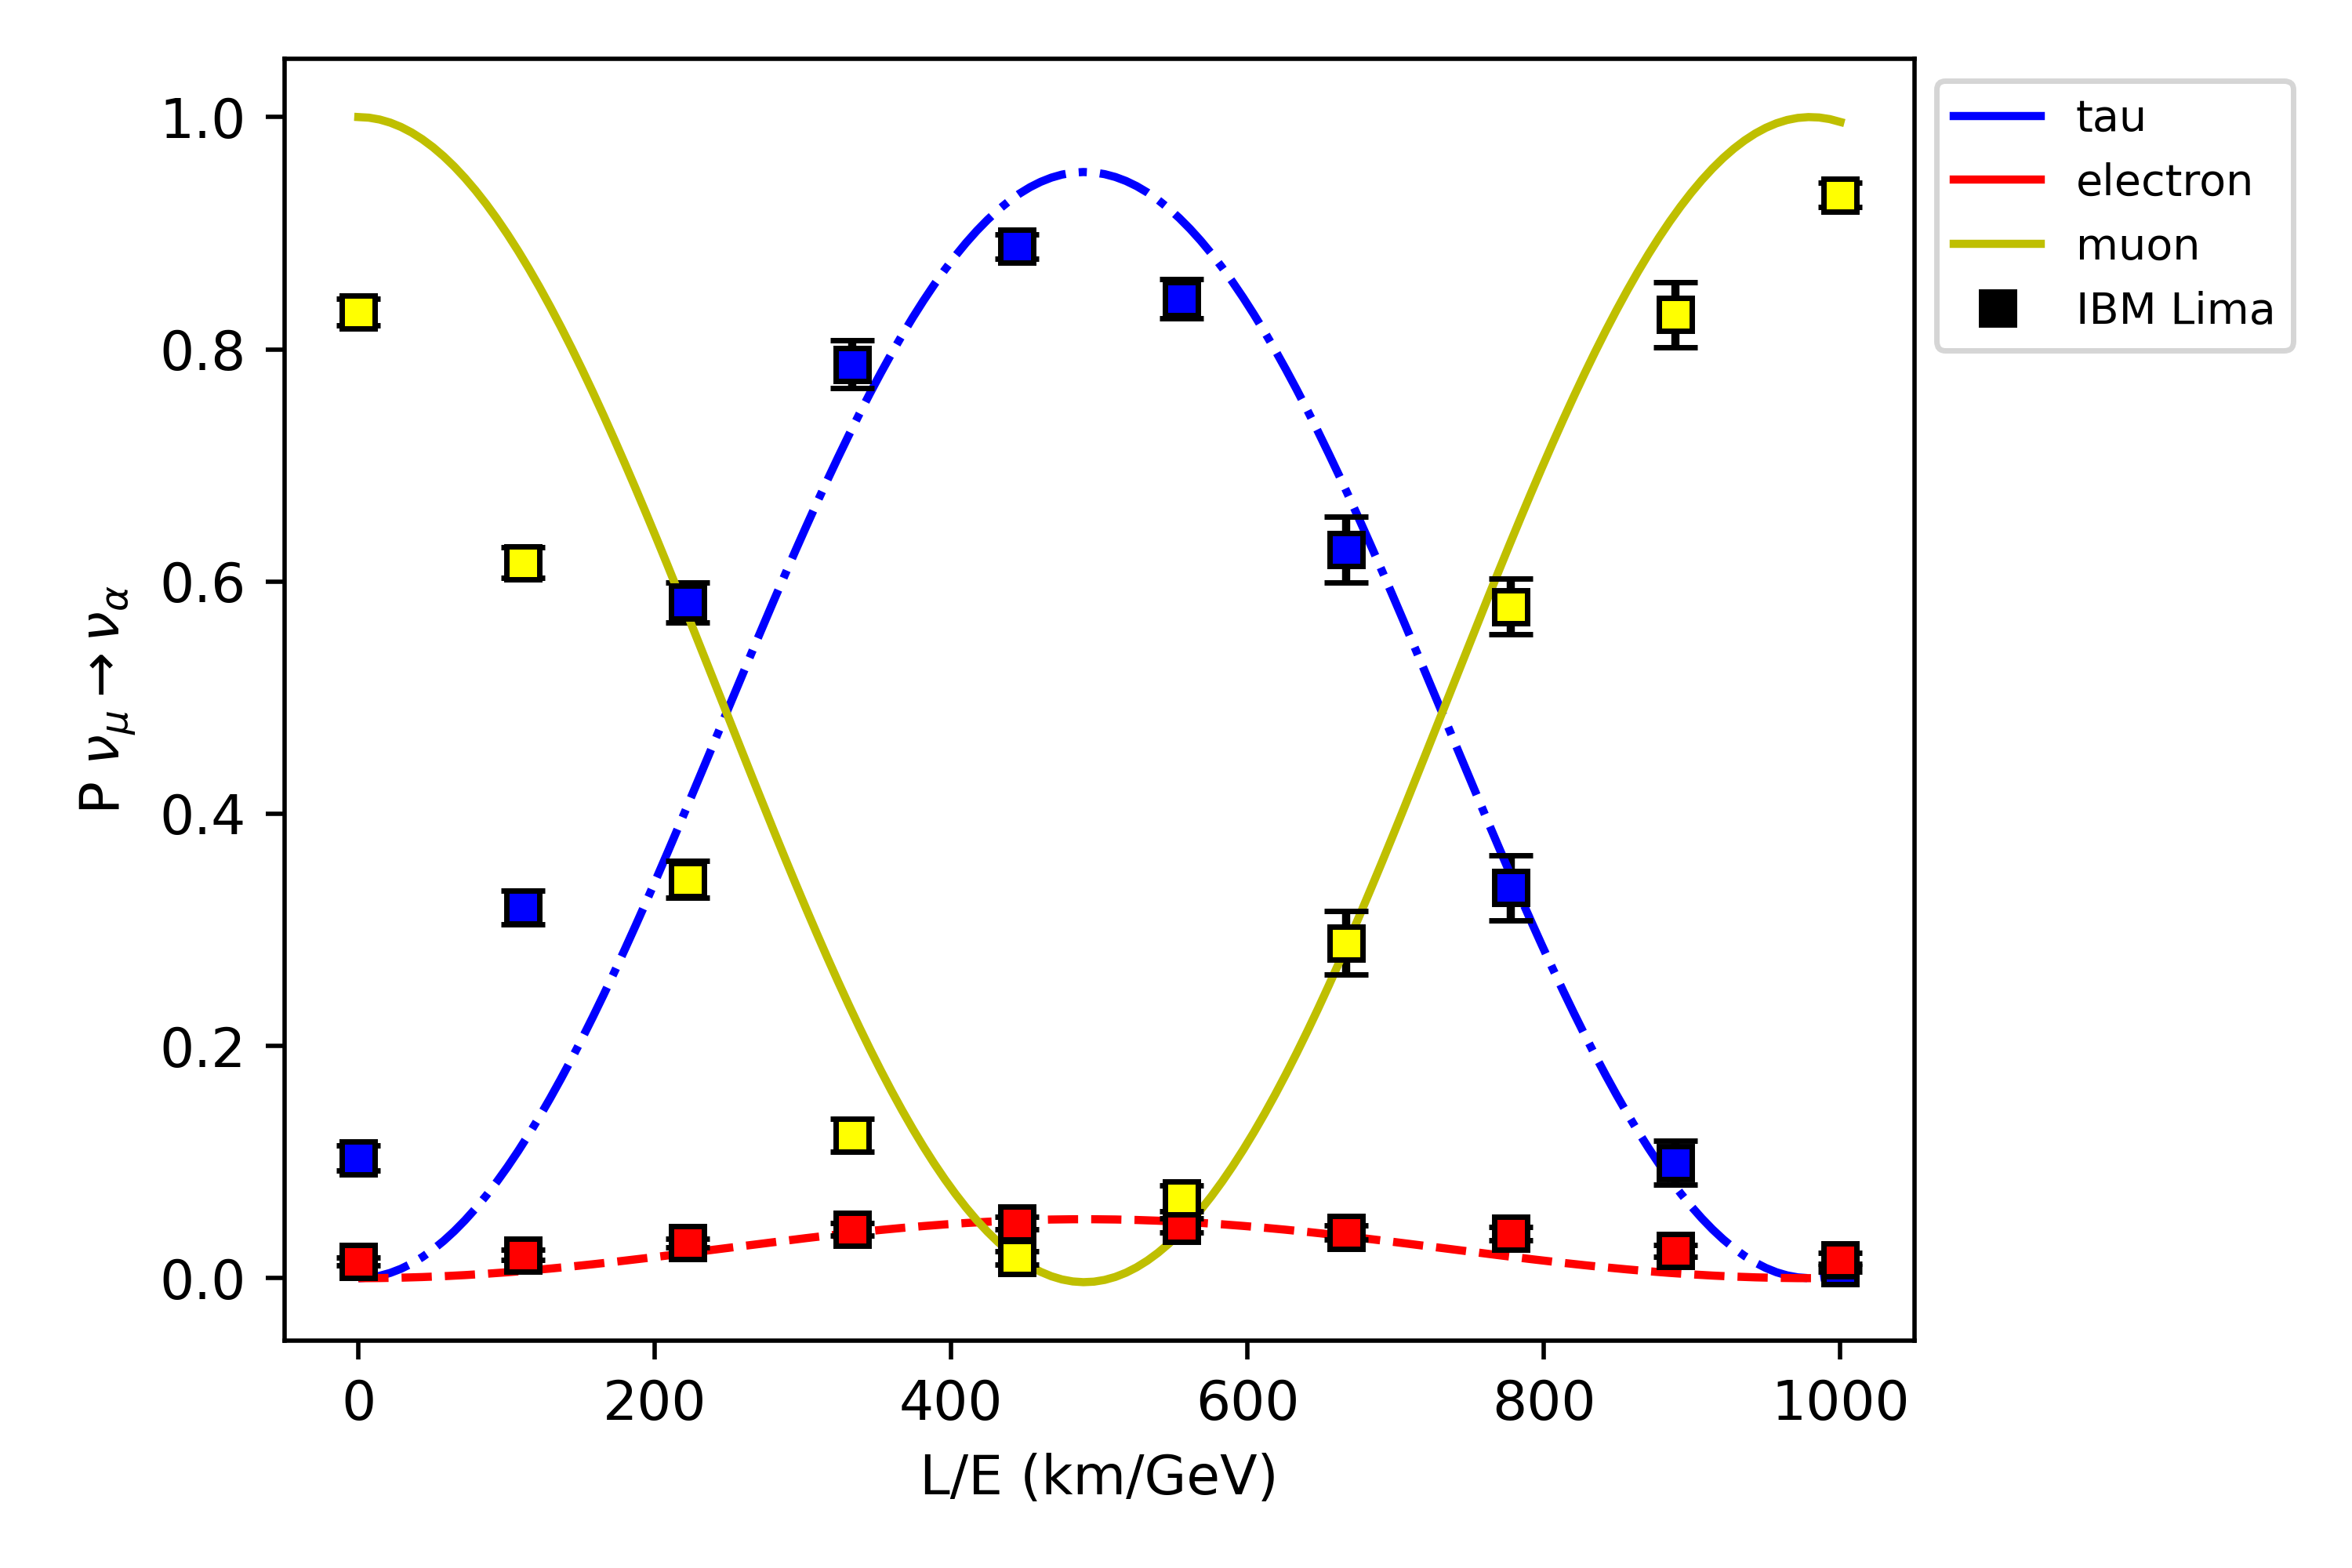
\includegraphics[scale=0.8]{fig_9.png}}
	\caption{Three flavour oscillation probability as function of time (in Quantum computer) }
	\label{fig 9}
\end{figure}\par system will be an entangled pure state.
\end{enumerate}
$c_{i}$ are called called Schmidt coefficients. Similarly, $\ket{\psi_{i}^{A}}$ and $\ket{\psi_{i}^{B}}$ are called Schmidt bases.
\subsubsection{ Pure and Mixed Entangled State}
For any composite system, a pure state is said to be entangled if the parts of the system are not pure states \cite{wootters}. That is, the whole system will be a pure state, but the individual subsystems will be mixed states. This property arises as a consequence of entanglement. When two systems get entangled, we cannot specify the state of a single system alone. The state of one system depends on the other system and vice versa. Similarly, one can define the concept of entanglement for mixed quantum states also. A mixed state is entangled if it cannot be represented as a mixture of unentangled pure states
\section{Entanglement Entropy}
In the later section, we saw how entanglement is related to the mixedness of the subsystems. Exploiting this feature of the entangled system, we can define a measure for entanglement. For bi-partite systems that are in a pure state, a single widely accepted measurement is the entropy of the entanglement. But for mixed entangled states, there is no unique measurement. The three most common measurements used in the case of mixed states are Entanglement of formation, Distillable entanglement, Relative entropy of entanglement. One can construct numerous other types of measurement from these three.\par
In the case of a pure state, von Neumann entropy is the most adequate measurement of the entanglement \cite{bennet96c}. Given the density matrix of a system to be $\rho$, the von Neumann entropy of the system is defined as,
\begin{equation}
S = -Tr(\rho\log\rho)
\end{equation}
where ``Tr" indicates Trace. The bi-partite von Neumann entropy is defined as the von Neumann entropy of the individual subsystems.
\begin{equation}
S(\rho_{A}) = -Tr(\rho_{A}\log\rho_{A}) =  -Tr(\rho_{B}\log\rho_{B})=S(\rho_{B})
\end{equation}
where, $\rho_{A}=Tr_{B}(\rho_{AB})$ and $\rho_{B}=Tr_{A}(\rho_{AB})$. Here $\rho_{A}$ and $\rho_{B}$ are the called the reduced density matrix of the composite system ($\rho_{AB}$). For a system in product state, individual subsystems would be pure state i.e, state of system can be written as tensor product of two pure state. Thus von Nuemann entropy of such system would be zero. For an entangled state, subsystems would be in a mixed state. Thus the von Neumann entropy would be non zero. In short,
\begin{enumerate}
    \item If $S(\rho)= 0$, state of system would be pure product state.
    \item If $S(\rho)\neq 0$, state of system would be pure entangled state.
\end{enumerate}
\section{Measurement of Entanglement in Neutrinos}
Bipartite entanglement is quantified efficiently by von Neumann entropy. Also any monotonic functions of the former can itself act as a measure. Discussions about such entanglement monotones can be found in \cite{horodecki}\cite{amico}. Linear entropy belongs to this class of entanglement monotones. Linear entropy can be considered lower order approximation to von Neumann entropy. The bipartite linear entropy $S_{L}$ is defined as the linear entropy of the either of its reduced state (they can be shown equal). For system whose state represented by density matrix $\rho$, Linear entropy is defined as,
\begin{equation}
S_{L} = \frac{d}{d-1}(1-Tr(\rho^{2}))
\end{equation}
More formal definition of linear entropy of a pure state $\ket{\psi}$ is provided by Blasone \emph{et.al} (2009) . It is as follows,\par
\emph{Consider a $N$-partite system $S=\{S_{1},S_{2},S_{3}....,S_{N}\}$. Now let us bipartite the system in to two-subsystems $S_{A}$ and $S_{B}$. Here $S_{A_{n}}=\{S_{i1},S_{i2},...S_{in}\}$, with $1\leq i_{1}<i_{2}<....<i_{n}\leq N$ ($1 \leq n < N$), and $S_{B_{N-n}} =\{S_{j1},S_{j2},....,S_{j(N-n)}\}$, with $1\leq j_{1}< j_{2} < ....<j_{N-n}$ ,and $i_{q} \neq j_{p}$. Let the density matrix of the system be $\rho_{AB}=\ket{\psi}\bra{\psi}$. Then $\rho_{A_{n}}= Tr_{B_{N-n}}(\rho_{AB})$ denotes the reduced density matrix of subsystem $S_{A_{n}}$ after tracing over subsystem $S_{B_{N-n}}$. The linear entropy of such a bi-partitioned system is defined as
\begin{equation}
\label{eq:25}
    S_{L}^{(A_{n}|B_{N-n})} (\rho_{AB}) = \frac{d}{d-1}\left(1-Tr_{A_{n}}(\rho_{A_{n}}^{2})\right)
\end{equation}
where d is the Hilbert-space dimension given by $d=min[dim S_{A_{N}},dim S_{B_{N-n}}]= min[2^{n},2^{N-n}]$}\cite{blasone2009}.\par

We can also define average linear entropy as:
\begin{equation}
\langle S_{L}^{(n:N-n)}(\rho_{AB})\rangle= \binom{N}{n}^{-1} \sum_{A_{n}} S_{L}^{(A_{n};B_{N-n})}(\rho_{AB})
\end{equation}
The value of linear entropy varies between $0$ to $1$. For a product state, value of linear entropy would be zero. For an entangled state, value of linear entropy would be non-zero. The state of the system will be maximally entangled if Linear entropy $S_{L}=1$.

\subsubsection{Linear Entropy of Neutrino States}\label{len}
As mentioned in the previous section, the state $\ket{\nu_{\alpha}(t)}$ is a pure state. Thus we can use linear entropy to quantify the entanglement in the system. First consider the two flavour case. Such a system shows bipartite entanglement. In particular we are taking electron-muon system (as they are used in simulation). For such a system, time evolved state is given by the equation ($\ref{eq:23}$).
\begin{gather}
\ket{\nu_{\alpha}(t)}=\Tilde{\textbf{U}}_{\alpha e}(t) \ket{1}_{\nu_{e}}\ket{0}_{\nu_{\mu}}+\Tilde{\textbf{U}}_{\alpha \mu}(t) \ket{0}_{\nu_{e}}\ket{1}_{\nu_{\mu}}    
\end{gather}
where the coefficients $\Tilde{\textbf{U}}_{\alpha \beta}$ is given by the equation ($\ref{eq:21b}$). 
For such a state, the density matrix will be $\rho_{\alpha}=\ket{\nu_{\alpha} (t)}\bra{\nu_{\alpha} (t)}$. Using equation ($\ref{eq:25}$), we can straight forwardly calculate linear entropy by tracing over one of the modes.
\begin{equation}
  \begin{split}
S_{L\alpha}^{(e;\mu)} = S_{L\alpha}^{(\mu;e)}&=4|\Tilde{\textbf{U}}_{\alpha e}(t)|^{2}|\Tilde{\textbf{U}}_{\alpha \mu}(t)|^{2} \\
&=4|\Tilde{\textbf{U}}_{\alpha e}(t)|^{2}(1-|\Tilde{\textbf{U}}_{\alpha e}(t)|^{2})\\
&=4|\Tilde{\textbf{U}}_{\alpha \mu}(t)|^{2}(1-|\Tilde{\textbf{U}}_{\alpha \mu}(t)|^{2})\\
  \end{split}  
\end{equation}
where, $S_{L\alpha}^{(e;\mu)} \equiv S_{L}^{(e;\mu)}(\rho^{(\alpha)})$. Here $\alpha$ refers the time evolved channel and the superscripts $(e;\mu)$ refers to flavour modes considered (here it is electron and muon flavours).\par
As we move from two-flavour to three-flavour case, we deal with multipartite entanglement (more than 2 modes). Still we can quantify the entanglement using some bipartite measures. Global entanglement is such a measure. The sum of all two-qubit entanglements between a single subsystem and each of the others is referred to as global entanglement. This can be expressed as average subsystem linear entropy. Thus it can be generalised as the sum of average linear entropies of all the possible bi-partitions of the system \cite{amico}\cite{brennen}.\par
For three flavour oscillations, linear entropy is given by,
\begin{equation}
\begin{split}
S_{L\alpha}^{(e,\mu;\tau)}& = 4|\Tilde{\textbf{U}}_{\alpha \tau}(t)|^{2}(|\Tilde{\textbf{U}}_{\alpha \mu}(t)|^{2} + |\Tilde{\textbf{U}}_{\alpha e}(t)|^{2})\\
S_{L\alpha}^{(e,\mu;\tau)}&=  4|\Tilde{\textbf{U}}_{\alpha \tau}(t)|^{2}(1-|\Tilde{\textbf{U}}_{\alpha \tau}(t)|^{2})
\end{split}
\end{equation}
Here tracing is done over mode $\tau$ and linear entropies of other bi-partitions can be obtained by permuting over the indices e, $\mu$. They are, 
\begin{equation}
\begin{split}
S_{L\alpha}^{(\mu,\tau;e)}&=  4|\Tilde{\textbf{U}}_{\alpha e}(t)|^{2}(1-|\Tilde{\textbf{U}}_{\alpha e}(t)|^{2})\\
S_{L\alpha}^{(\tau,e;\mu)}&=  4|\Tilde{\textbf{U}}_{\alpha \mu}(t)|^{2}(1-|\Tilde{\textbf{U}}_{\alpha \mu}(t)|^{2})
\end{split}
\end{equation}
The average linear entropy in the three-flavour case is given by,
\begin{equation}
\label{eq:26}
    \langle S_{L\alpha}^{(2:1)}\rangle = \frac{8}{3}(|\Tilde{\textbf{U}}_{\alpha e}(t)|^{2}|\Tilde{\textbf{U}}_{\alpha \mu}(t)|^{2} + |\Tilde{\textbf{U}}_{\alpha e}(t)|^{2}|\Tilde{\textbf{U}}_{\alpha \tau}(t)|^{2} + |\Tilde{\textbf{U}}_{\alpha \mu}(t)|^{2}|\Tilde{\textbf{U}}_{\alpha \tau}(t)|^{2})
\end{equation}
The equation ($\ref{eq:26}$) gives us the global entanglement of the three-flavor system. Thus using linear entropy we can effectively quantify the entanglement in neutrino.


\newpage
\thispagestyle{empty}
\mbox{}
\newpage
\chapter{Neutrino Oscillation in a quantum processor}\label{sec4}
Spontaneous transition of neutrino flavour over a macroscopic distance occurs due to the non-coincidence of flavour and mass eigenstates called Neutrino Oscillation.  Neutrino oscillation through its periodic nature has given insights that neutrinos have non zero mass, which is something beyond the Standard Model’s predictions. Thus neutrino oscillations indicate the existence of physics beyond the standard model. Experimentally when we study neutrino oscillation what we do inspect the neutrino oscillation behaviour at different values of energies $E$ and baseline $L$. For different $\frac{L}{E}$ values, we perform either appearance experiment (or disappearance experiment) and get appearance probability ( or disappearance probability). Using experimentally obtained probabilities we would fix the values of the mixing angle ($\theta_{ij}$) and squared mass difference ($\Delta m_{ij}^{2}$) by putting them back into the corresponding equation. \par
Experimental detection of neutrino oscillation would require sophisticated instruments. Often the labs are kept underground. This is to prevent interference due to cosmic rays. We cannot detect all flavours using single type of detector.  Detectors depending on the type, work at different energy range and threshold energy below which detection of neutrinos is not possible. For example, detectors using water as detector material, detect neutrinos via elastic scattering will not work for neutrinos of low energy ($< 5 MeV$). Similarly, Chlorine-based detectors have a threshold of 0.814 MeV.\par
Another thing that often concerns the experimentalist is the sensitivity of the detectors. In the case of reactor-based or accelerator-based experiments sensitivity of the detector depends upon the baseline length. For e.g., for a neutrino beam of energy $E \sim 1 GeV$ detector baseline should be at least of the order of $10^{4}$  for it to be sensitive to $\Delta m_{ij}^{2}$ down to $\sim 10^{-4} eV^{2}$. So we need to produce high energetic neutrino beams to reduce the baseline without compromising sensitivity. In such a scenario simulation studies aid us. Using the experimentally determined parameters, we can perform simulation studies of the flavour oscillation for neutrino beams of energies inaccessible under lab conditions.\par
Not so long after Feynman put forward the idea of simulating a quantum system with another, the possibility of using a quantum computer to simulate quantum systems was understood. The major difference between a classical computer and a quantum computer in simulating quantum systems is that the quantum computer performs actual Hamiltonian evolution whereas others just emulate it. At the present stage, even though the result got by quantum simulations is not praiseworthy as that of classical simulations, the computational cost of quantum algorithms are much less compared to classical algorithms for simulating a quantum system. The development of fault tolerant quantum computation would give us more reliable results and enable us to manoeuvre the quantum advantage in a wide variety of fields.\par
Here we perform quantum simulation by executing an analogous Hamiltonian evolution to generate neutrino flavour oscillation. Such encoding and evolution is a stepping stone towards developing more advanced quantum simulations of neutrino oscillation. Systems that could particularly benefit from the quantum algorithmic approach to neutrino flavour evolution include those where collective neutrino oscillations are relevant, such as in Supernovae or the early Universe \cite{jones}. In such cases, the quantum Boltzmann equation which gives the evolution neutrino population can only be solved approximately. \par
In this section, we are going to first discuss how to encode two neutrino system evolution on a quantum computer using only a single qubit. Then we extend this idea to implement three flavour oscillation in a two qubit space inside a quantum processor. While simulating, the primary challenge that lies ahead is to implement the PMNS matrix which relates the flavour and mass eigenstates. Here we use the algorithm or the circuit put forward by Arg\"uelles \emph{et.al} 2019, to study neutrino flavour oscillation. This algorithm uses quantum gates to realise the PMNS matrix and to realise the time evolution operator. The algorithm is discussed below.
\section{Simulation of Two Flavour Oscillation}\label{2FO}
In this circuit we only use a single qubit to encode neutrino flavour state and to time evolution of the states we apply corresponding quantum gates. Consider our system have of two neutrino flavour state let say $\alpha$ and $\beta$. Now we want to encode these states on qubits and encoding scheme we follow is given below.
\begin{equation}
\begin{split} 
\label{eq:14}
\ket{\nu_{\alpha}}=\begin{bmatrix} 1 \\ 0 \end{bmatrix} , 
\ket{\nu_{\beta}}=\begin{bmatrix} 0 \\ 1 \end{bmatrix}
\end{split}
\end{equation}
In the case of two flavour oscillation is the PMNS matrix is given by the 2x2 rotation matrix.
\begin{equation}
U=\begin{bmatrix} \cos\theta & \sin\theta \\ -\sin\theta & 
\cos\theta \end{bmatrix}
\end{equation}
PMNS operation is encoded in  IBM Quantum computer by three-parameter U gate. The matrix form of the gate is given as :
\begin{equation}
	\label{eq:15}
	U (\Theta,\Phi,\Lambda) =\begin{bmatrix} \cos\left(\frac{\Theta}{2}\right) & -\sin\left(\frac{\Theta}{2}\right)e^{i\Lambda} \\ \sin\left(\frac{\Theta}{2}\right)e^{i\Phi} & 
		\cos\left(\frac{\Theta}{2}\right)e^{i(\Lambda + \Phi)} \end{bmatrix}
\end{equation}

For a two-neutrino system, the oscillation probabilities depend upon a single parameter known as mixing angle. Thus the $U$ gate which having $3$ parameters has to be modified,
\begin{enumerate}
	\item Now consider the case of including the parameter $\Phi$. This corresponds to the re-phasing of charged lepton field, and standard Lagrangian is invariant under such an operation. For e.g., let us consider the case of a muon neutrino. The presence of $\Phi$ corresponds to re-phasing $\ket{\nu_{\mu}}$ by $e^{-i\Phi}\ket{\nu_{\mu}}$. As said before, under such a transformation Lagrangian remains invariant and does not influence oscillation probabilities \cite{giunti2007}. Thus we can take $\Phi=0$ without loss of any generality.
	\item We can use the same arguments provided above to set $\Lambda = 0$ for the case of Dirac fermions \cite{giunti2007}. But this is not possible in the case of neutrino being a Majorana particle. For Majorana particle, this phase is physical and should be maintained in the Lagrangian. However, it is proven that the presence of such a phase would not affect the oscillation probabilities \cite{giunti2010} and thus can be taken equal to zero while studying the neutrino oscillation irrespective of the type of particle.
\end{enumerate}
Thus using a $U$ gate we can realise the PMNS matrix by suitably choosing the value of the parameters. 
\begin{equation}
\label{eq:16}
U_{PMNS}^{2\times2} = U(-2\theta,0,0) = \begin{bmatrix} \cos\theta & \sin\theta \\ -\sin\theta & 
\cos\theta \end{bmatrix}
\end{equation}
Where $\theta$ is the mixing angle.\par

Using the PMNS matrix that we realised using U gate, flavour state encoded in the qubit equation ($\ref{eq:14}$) can be rotated into in the mass basis \{$\ket{\nu_{1}},\ket{\nu_{2}}$\}. After rotating into mass basis we have to time evolve the mass states. From equation ($\ref{eq:1}$) we know that,
\begin{gather*}
\begin{split}
\ket{\nu_{\alpha}(t)}& = U_{\alpha 1}^{\dagger}e^{i\phi_{1}}\ket{\nu_{1}} + U_{\alpha 2}^{\dagger}e^{i\phi_{2}}\ket{\nu_{2}}\\
&=e^{i\phi_{1}}( U_{\alpha 1}^{\dagger}\ket{\nu_{1}} + U_{\alpha 2}^{\dagger} e^{ i\Delta\phi}\ket{\nu_{2}}
\end{split}
\end{gather*}
Where $\Delta\phi= \phi_{2}-\phi_{1}$. Now, lose the delta sign, $\Delta{\phi} \equiv \phi$. Global phases like $e^{i\phi_{1}}$ have no physical significance and can be discarded \cite{Benenti}, relative phases between mass states are only relevant for neutrino oscillations, and without loosing any generality we can measure all phases relative to $\ket{\nu_{1}}$ state. Thus time evolution operator can also be encoded by using a $U$ gate.
\begin{equation}
\textbf{U}(t) = U(0,0,\phi) = \begin{bmatrix} 1 & 0 \\ 0 & e^{i\phi} \end{bmatrix}
\end{equation}
Where $\phi = \frac {\Delta m^{2} t}{2E\hbar}$ (equation (\ref{eq:6}-\ref{eq:6a})) in natural units and under ultra-relativistic approximation.\par
After time evolving the mass states it is rotated again back into flavour basis using applying $U$ gates and is measured to get back the final state. Note that by simply changing parameter $\theta \rightarrow -\theta$ in the equation ($\ref{eq:16}$), $U^{\dagger}$ can be constructed out of $U$ gate. 
\begin{equation}
U_{PMNS}^{2x2 \ \dagger}= U(2\theta,0,0) = \begin{bmatrix} \cos\theta & -\sin\theta \\ \sin\theta & \cos\theta \end{bmatrix}
\end{equation}
\begin{figure}[h]
\graphicspath{ {./Images/} }
\centering	
{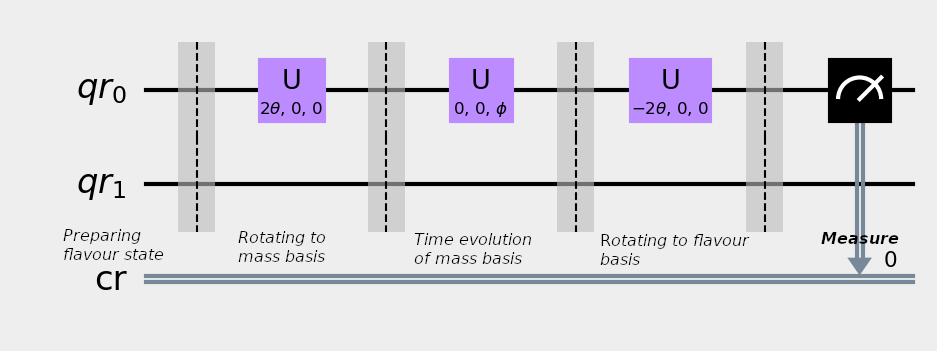
\includegraphics[width=\textwidth]{fig_2.png}}
\caption{Circuit simulating two flavour oscillation\cite{jones}}
\label{fig 2}
\end{figure}
\begin{comment}
Thus using a U gate we can realise the PMNS matrix by suitably choosing the value of the parameters. 
\begin{equation}
\label{eq:16}
U_{PMNS}^{2x2} = U(2\theta,0,0) = \begin{bmatrix} cos(\theta) &- \sin(\theta) \\ sin(\theta) & 
cos(\theta) \end{bmatrix}
\end{equation}
Where $\theta$ is the mixing angle and is determined by experimentally.\par

Applying the PMNS matrix that we realised using U gate to flavour state encoded in the qubit $\ref{eq:14}$ we can rotate it into in the mass basis ($\ket{\nu_{1}},\ket{\nu_{2}}$). Then, for witnessing the neutrino oscillation we have to time evolve the mass states. 
\begin{gather*}
\begin{split}
\ket{\nu_{\alpha}(t=0)}& = U_{\alpha 1}\ket{\nu_{1}} + U_{\alpha 2}\ket{\nu_{2}}  \\
\ket{\nu_{\alpha}(t)}& = U_{\alpha 1}e^{i\phi_{1}}\ket{\nu_{1}} + U_{\alpha 2}e^{i\phi_{2}}\ket{\nu_{2}}\\
&=e^{i\phi_{1}}( U_{\alpha 1}\ket{\nu_{1}} + U_{\alpha 2} e^{ i\Delta\phi}\ket{\nu_{2}}
\end{split}
\end{gather*}
Where $\Delta\phi=\phi = \phi_{2}-\phi_{1}$.
Global phases like $e^{i\phi_{1}}$ have no physical significance and can be discarded\cite{benenti}, relative phases between mass states are only relevant for neutrino oscillations, and without losing any generality we can measure all phases relative to $\ket{\nu_{1}}$ state. The time evolution operator can also be encoded by using a U gate.
\begin{equation}
\textbf{U(t)} = U(0,0,\phi) = \begin{bmatrix} 1 & 0 \\ 0 & e^{i\phi} \end{bmatrix}
\end{equation}
Where $\phi = \frac {\Delta m^{2} t}{2E}$ ( refer \ref{eq:6} ,\ref{eq:6a}) in natural units and under ultra relativistic approximation.\par
After time evolving the mass states it is rotated again back into flavour basis by applying $U^{\dagger}$ and is measured to get back the final state. By simply changing parameter $\theta \rightarrow -\theta$ in $\ref{eq:16}$, $U^{\dagger}$ can be encoded using U gate. 
\begin{equation}
U_{PMNS}^{2x2 \ \dagger}= U(-2\theta,0,0) = \begin{bmatrix} cos(\theta) & \sin(\theta) \\ -sin(\theta) & cos(\theta) \end{bmatrix}
\end{equation}

\end{comment}

\section{Simulation of Three Flavour Neutrino Oscillation}\label{3FO}
Using only one qubit, we can only construct a Hilbert space of dimension two. A three flavour neutrino oscillation involves a dimension of $3$ and requires more than one qubit. So ,three flavours of neutrino are encoded by using $two$ qubits. The encoding scheme we follow is that,
\begin{equation}
\label{eq:17}
\begin{split}
\ket{\nu_{e}}& = \ket{00} = \begin{bmatrix} 1\\0\\0\\0 \end{bmatrix}, \ \ket{\nu_{\tau}} = \ket{01} = \begin{bmatrix} 0\\1\\0\\0 \end{bmatrix} \\
\ket{\nu_{\mu}}&=\ket{10}=\begin{bmatrix} 0\\0\\1\\0 \end{bmatrix}, \ \ket{\nu_{x}} = \ket{11} = \begin{bmatrix} 0\\0\\0\\1 \end{bmatrix} 
\end{split}
\end{equation}
There is one redundant basis state  $\ket{\nu_{x}}$ in this encoding. This could represent the fourth flavour of neutrino in models with sterile neutrinos. But for our discussion, we consider it as physically decoupled and thus unphysical. The circuit is designed in such a way that fourth state does not take part in oscillation. Here also we follow the same methodology as discussed in the two flavour case. We prepare flavour states and do the unitary transformation of flavour state into mass basis, then time evolve the mass states and transform it back into flavour basis and measure it. Now, realising the PMNS matrix using quantum gates is not trivial as in the case of two flavour case. Here we follow the circuit proposed by Arg\"uelles and Jones (2019)\cite{jones}, in which $U$ gates and $CNOT$ gates are used for realising the PMNS matrix. 
\begin{figure}[h]
\graphicspath{ {./Images/} }
\centering	
{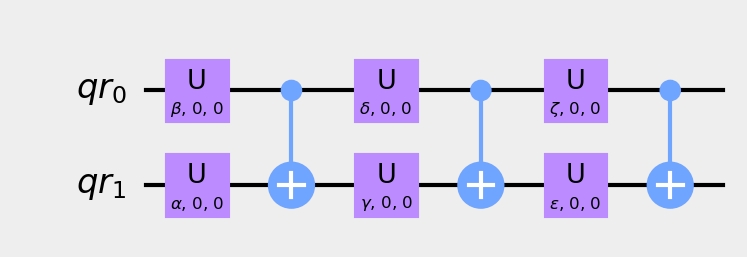
\includegraphics[scale=1]{fig_3.png}}
\caption{Gate arrangement for realizing PMNS matrix\cite{jones}}
\label{fig 3}
\end{figure}

The circuit in the figure $\ref{fig 3}$ is designed in such a way as to mimic the action of the PMNS matrix. To fix the free parameters on this circuit, the circuit is mapped onto a matrix multiplication on the computational basis. A numerical fit is then performed to match the experimentally determined PMNS matrix. The input values of the PMNS matrix used to fit the parameters are from \cite{estaban} and are,
\begin{equation}
U_{PMNS} = \begin{bmatrix} 0.821427 & 0.550313 & 0.149708 & 0 \\ -0.481513&0.528538&0.699138&0\\0.305618&-0.646377&0.699138&0\\0&0&0&1 \end{bmatrix}
\end{equation}
Here we consider the PMNS matrix of $4\times4$ form since the encoding scheme uses $2$-qubit which forms $4$-dimensional Hilbert space.  The last row represents decoupled physical state and will not take part in flavour oscillation. \par
The PMNS matrix is fitted by the method of gradient minimization over the six parameters (sum of squared residuals of each element of the matrix is minimised). The best fit parameter provided in \cite{jones} are, 
\begin{equation}
\label{eq:18}
\alpha = -0.6031,\ \beta = -2.0125, \ \gamma = -0.7966, \ \delta = 1.0139 ,\  \epsilon = 0.7053, \ \zeta = 1.3599
\end{equation}

Substitution of parameters given by the equation ($\ref{eq:18}$) in the circuit would give us PMNS matrix and PMNS$^{\dagger}$ is got by inverting the gate arrangement.\par
The evolution operation $\textbf{U}(t)$ in computational basis is given by,
\begin{equation}
\textbf{U}(t)=\exp [i \ diag(0,\Delta m_{12}^{2}\frac{t}{2E\hbar}, \Delta m_{13}^{2}\frac{t}{2E\hbar},\Phi)]
\end{equation}
Where $\Phi$ is an arbitrary phase that can be picked up for convenience and can be discarded since fourth basis state is not observable. Such a time evolution operator is realised using two $U$ gates.
\begin{equation}
\textbf{U}(t)= U(0,0,\phi_{1})) \otimes U(0,0,\phi_{2})
\end{equation}
Where $\phi_{1}=\frac{\Delta m_{13}^{2}t}{2E\hbar}$ and $\phi_{2}=\frac{\Delta m_{12}^{2}t}{2E\hbar}$.\par
The circuit for simulating three flavour oscillation is given in the figure \ref{fig 4}.
\begin{figure}[H]
\graphicspath{ {./Images/} }
\centering	
{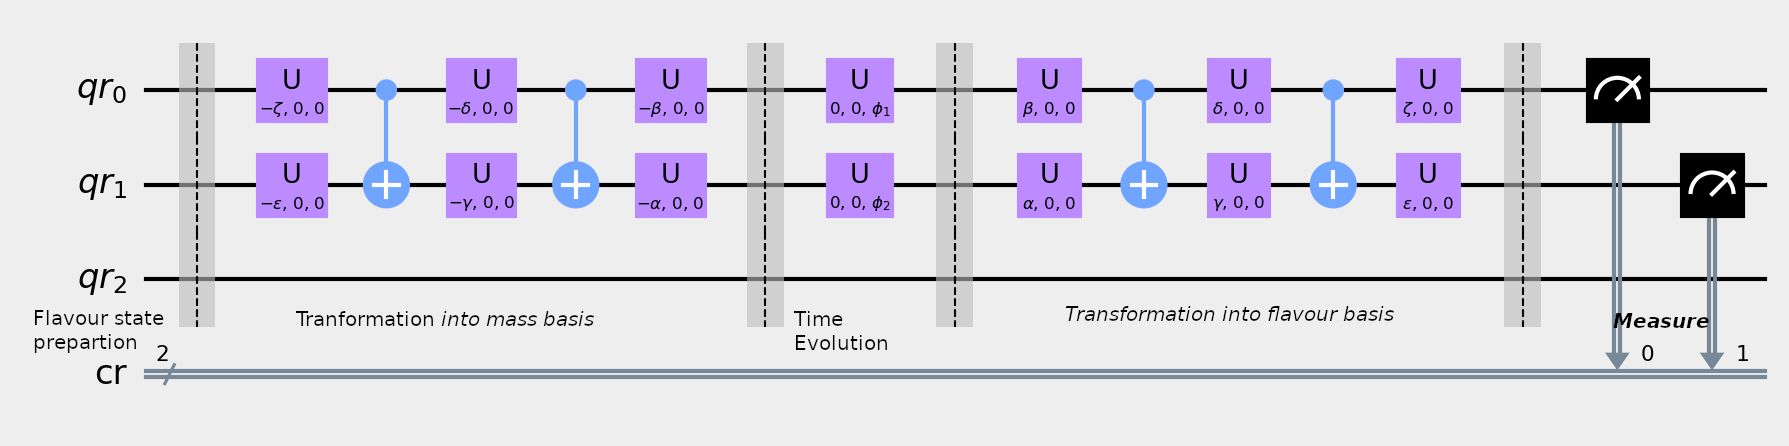
\includegraphics[width=\textwidth]{fig_4.png}}
\caption{Circuit for simulating three flavour oscillation\cite{jones}}
\label{fig 4}
\end{figure}

It should be noted that, this circuit is complex compared to two flavour case. Consequently read out errors and gate error will be larger compared to the former. Also this circuit can be also extended to incorporate sterile neutrinos and to study matter effects (MSW effects). Scheme for such studies are also provided in \cite{jones}.
\section{Measuring Entanglement Using Simulation}
For a two-flavour case, if the system we consider is electron-muon system, then linear entropy gives the entanglement in the system (refer section [$\ref{len}$]).
\begin{equation*}
    S_{L\alpha}^{(e;\mu)} = S_{L\alpha}^{(\mu;e)}=4|\Tilde{\textbf{U}}_{\alpha e}(t)|^{2}|\Tilde{\textbf{U}}_{\alpha \mu}(t)|^{2}
\end{equation*}
From equation ($\ref{eq:21b}$),
\begin{equation*}
P_{\nu_{\alpha} \rightarrow \nu_{\beta}}(t) = |\braket{\nu_{\beta}|\nu_{\alpha}(t)}|^{2} = |\Tilde{\textbf{U}}_{\alpha\beta}(t)|^{2}
\end{equation*}
Thus we can rewrite linear entropy as,
\begin{equation}
\begin{split}
\label{eq:27}
    S_{Le}^{(e;\mu)}& = S_{Le}^{(\mu;e)}=4 P_{ee}P_{e\mu}\\
    S_{L\mu}^{(e;\mu)}& = S_{L\mu}^{(\mu;e)}=4 P_{\mu e}P_{\mu\mu}
\end{split}
\end{equation}
Where $P_{\alpha \beta} = P_{\nu_{\alpha}\rightarrow\nu_{\beta}} = P_{\beta \alpha}$. We can get the apperance and disappearnce probability in $e-\mu$ system directly from the circuit given in the figure $\ref{fig 2}$. Substituting these values would give the linear entropy of the subsystems and thereby the entanglement of the system.\par
Similarly for three flavour case, 
\begin{equation}
\begin{split}
 S_{Le}^{(e,\mu;\tau)} &=4P_{e\tau}(P_{ee}+P_{e\mu})=4P_{e\tau}(1-P_{e\tau})\\
 S_{L\mu}^{(e,\mu;\tau)}& =4P_{\mu\tau}(P_{\mu e}+P_{\mu \mu})=4P_{\mu\tau}(1-4P_{\mu\tau})\\
 S_{L\tau}^{(e,\mu;\tau)}& =4P_{\tau\tau}(P_{\tau e}+P_{\tau \mu})=4P_{\tau\tau}(1-4P_{\tau\tau})\\
 \end{split}
\end{equation}
Similarly we found out equations for other bi-partitions by permuting over the indexes e,$\mu$,$\tau$.
From it, we can find out average linear entropy as,
\begin{equation}
\label{eq:28}
\begin{split}
    \langle S_{L e}^{(2:1)}\rangle &= \frac{8}{3}(P_{ee}P_{e\mu}+P_{ee}P_{e\tau}+P_{e\mu}P_{e\tau})\\
    \langle S_{L \mu}^{(2:1)}\rangle &= \frac{8}{3}(P_{\mu e}P_{\mu \mu}+P_{\mu e}P_{\mu\tau}+P_{\mu\mu}P_{\mu\tau})\\  
    \langle S_{L \tau}^{(2:1)}\rangle &= \frac{8}{3}(P_{\tau e}P_{\tau \mu}+P_{\tau e}P_{\tau\tau}+P_{\tau\mu}P_{\tau\tau})\\
    \end{split}
\end{equation}
This can be calculated using the circuit given in the figure $\ref{fig 4}$. Average linear entropy would give a measure of the global entanglement of the three-flavour system.

\newpage
\thispagestyle{empty}
\mbox{}
\newpage


\chapter{Simulation Results}\label{sec5}
We used IBM Quantum Experience which is a cloud-based computing service provided by IBM to run our circuits. IBM Q ( short form of IBM Quantum Experience) provides about 27 quantum services which comprise of 5 different types of simulators (including QASM Simulator) and 22 Quantum computers. Out of the 22 Quantum Computers, 9 are publicly accessible and the remaining are exclusive for the collaborators. Even though great advancement has been made in this field over the decade, still technology remains imperfect. Each gate applied to the circuit would induce an error of $\mathcal{O}(0.1\%)$. Readout error is of $\mathcal{O}(5\%)$ per qubit. Thus the error in the result increases as the length of the circuit, prohibiting reliable lengthy calculations. But one can use quantum error-correcting codes to mitigate the errors. 
\section{Two Flavour Oscillations: Simulation Results} 
With the quantum circuit defined in the section $\ref{2FO}$, we simulated an electron neutrino ($\nu_{e}$) disappearance experiment with the parameters given by the KamLAND experiment \cite{Eugichi}. Kamioka Liquid Scintillator Antineutrino Detector(KamLAND) is an electron antineutrino detector located in the Kamioka observatory. It studies neutrino oscillation using electron antineutrino produced by nuclear reactors.\cite{Iwamoto}.\par
\subsection{Simulation Using QASM Simulator}
Electron-neutrino state is encoded into $\ket{0}$ state. We ran 1024 trails and got back the neutrino state after time evolution. Then we perform projective measurement. By projective measurement we mean a case where the output state is projected in to the computational basis ($\{\ket{0},\ket{1}\}$). Thus the state is projected either to $\ket{0}$ or $\ket{1}$ depending upon output state. Here we run 1024 trails and takes the count of $\ket{0}$ state. From this count, disapperance probability of electron was calculated. The experiment was repeated for a range of neutrino beam energies and curve showing how disapperance probability varies with energy was plotted.\par
\begin{figure*}[h]
	\graphicspath{ {./Images/} }
	\centering	
	{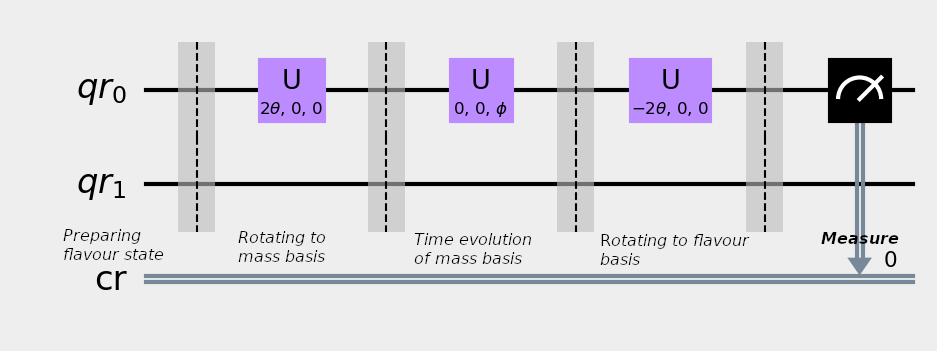
\includegraphics[width=0.7\textwidth]{fig_2.png}}
 \end{figure*}\par
We performed simulations for different values of neutrino beam energies while fixing the $L$ to be constant. We plotted how disappearance probability varies as a function of energy in MeV. It should be noted that we had chosen $L=180$ km in order to match the experimental conditions of the KamLAND. 
\begin{figure}[H]
	\graphicspath{ {./Images/} }
	\centering	
	{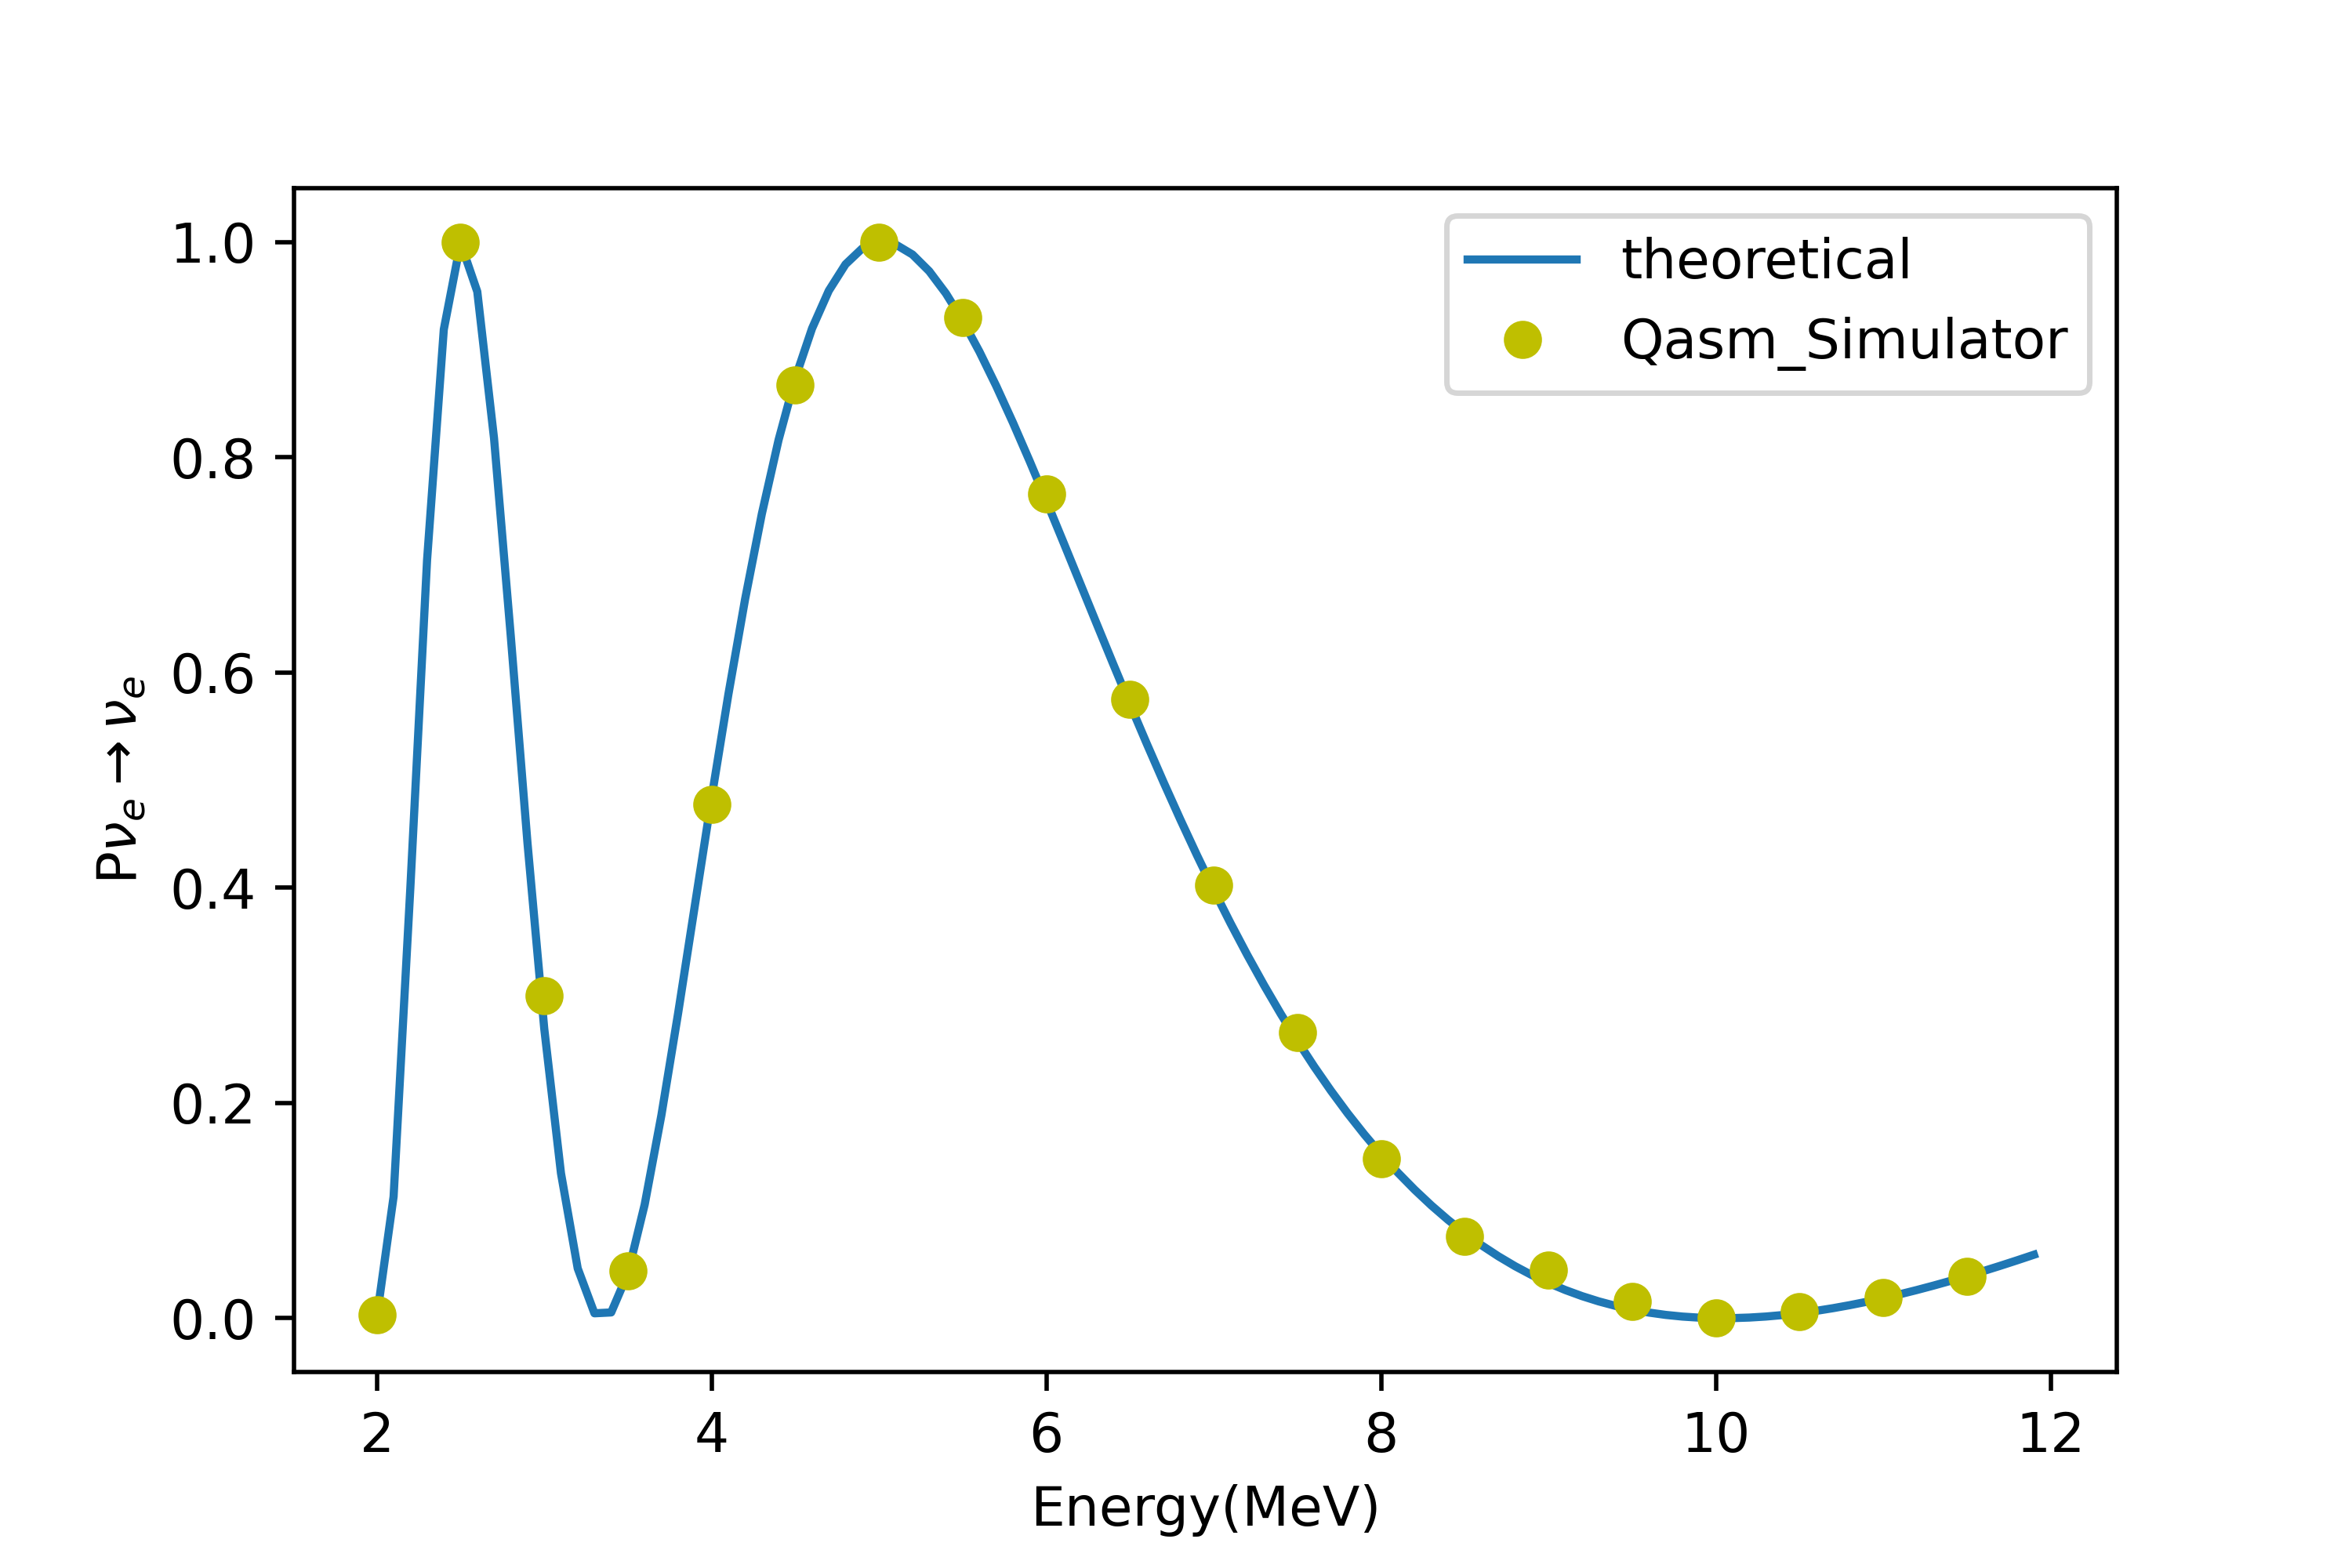
\includegraphics[width=0.8\textwidth]{fig_5.png}}
	\caption{Disappearance probability in $\nu_{e}-\nu_{\mu}$ system as a function of energy (in QASM simulator). }
	\label{fig 5}
\end{figure}
From the figure $\ref{fig 5}$ it is evident that our circuit performs very well and correctly predicts the disappearance probability. We were able to observe the sinusoidal variation of probability as predicticed by equation ($\ref{eq:14}$). In the QASM simulator circuit perform extremely well and predicts probability that agrees with the theoretical value.
\subsection{Simulation Using IBM Quantum Computer}
Circuit provided in figure $\ref{fig 2}$ is used to perform simulation in IBM Quantum computers. We performed the simulation on a IBM quantum computer named as IBM Armonk. It is a single qubit quantum computer which also supports pulse mode.\\

\begin{minipage}{0.5\textwidth}
\textbf{IBM Armonk}\\	
Quantum Volume : 1\\
Processor: Canary r1.2\\
Basis gates: ID, RZ, SX, X\\
\end{minipage}%
\begin{minipage}{0.5\textwidth}
Avg. CNOT Error: N/A\\
Avg. Readout Error: 3.160e-2\\
Avg. T1: 172.93 $\mu$s\\
Avg. T2: 344.85 $\mu$s
\end{minipage}

Like the former, we ran the circuit 1024 shots and found out neutrino counts. Using this counts we calculated the disapperance probability. 
\begin{figure}[H]
	\graphicspath{ {./Images/} }
	\centering	
	{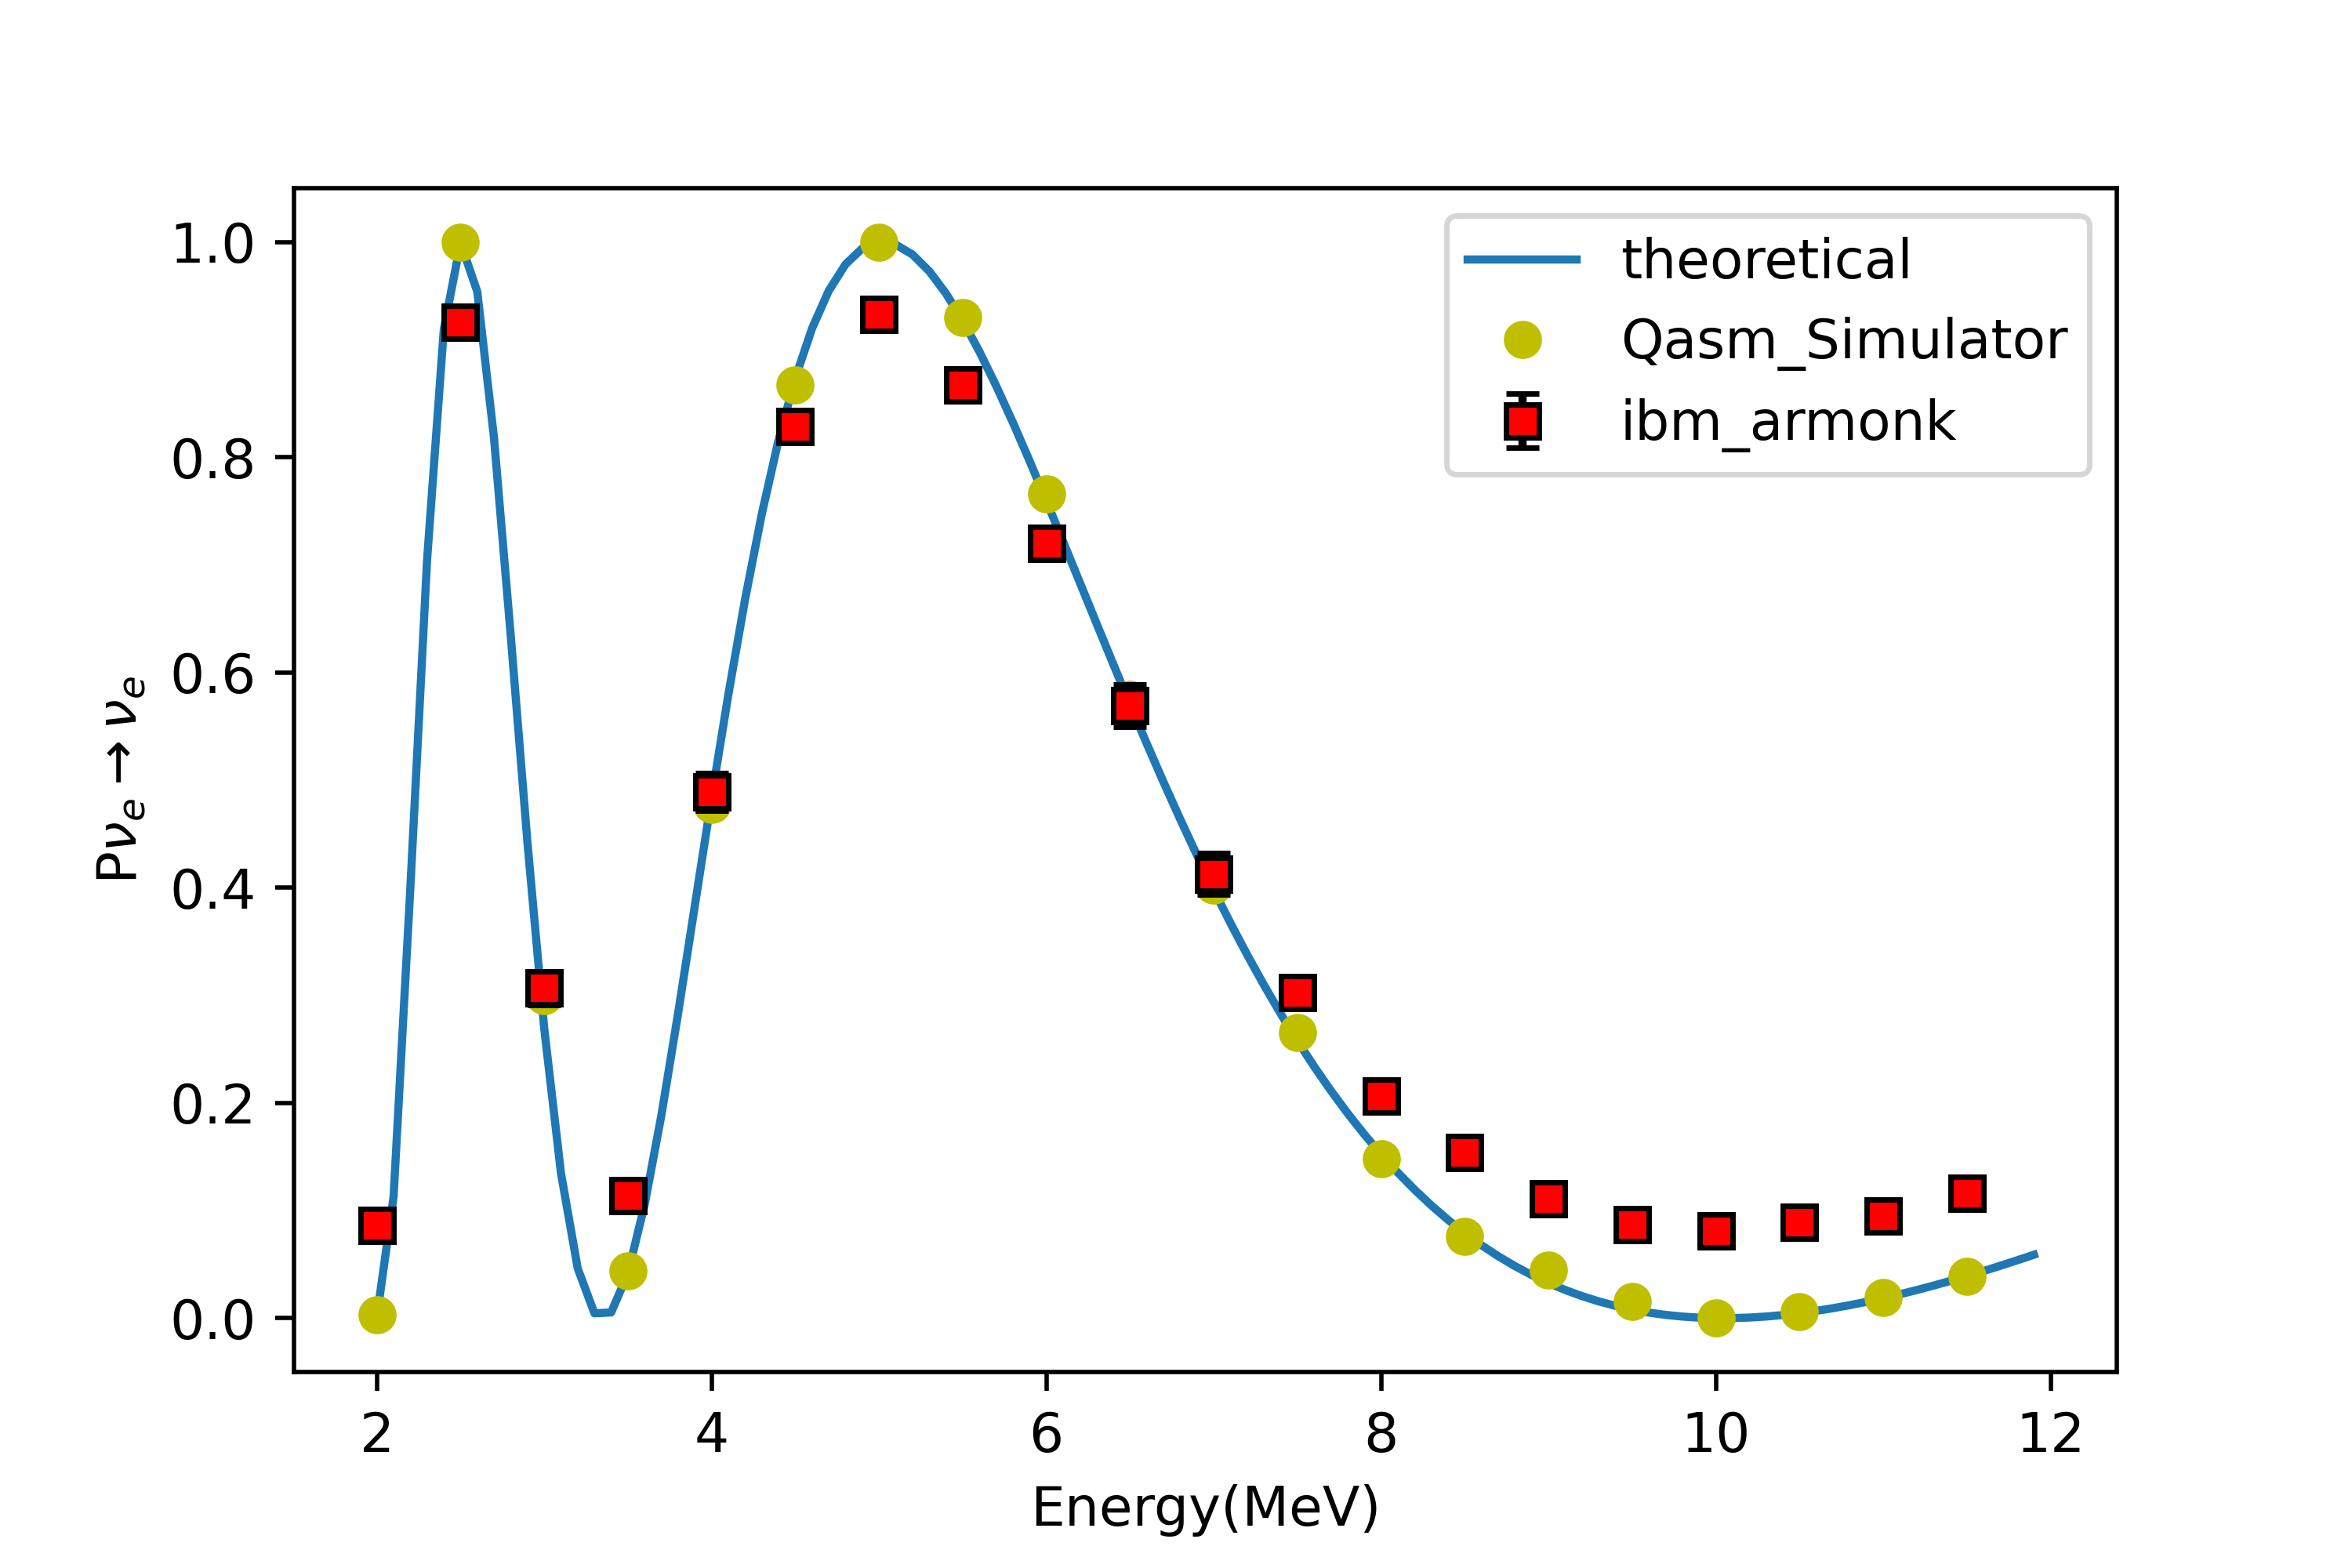
\includegraphics[scale=0.8]{fig_6.png}}
	\caption{Disappearance probability in $\nu_{e}-\nu_{\mu}$ system as a function of energy (in Quantum computer)}
	\label{fig 6}
\end{figure}\par
Here we also have to account for the statistical error that may happen while running circuits on actual quantum computers. For a particular value of energy we repeated the experiment 10 times and calculated standard deviations of data. From figure $\ref{fig 6}$ it is evident that the behaviour of theoretical curve by simulational results even though there is some error in value predicted by the circuit.
\pagebreak
\subsection{Entanglement Studies}
Through simulation using the circuit in figure $\ref{fig 2}$, we can get the disappearance and appearance probabilities in the $e-\mu$ system. By substituting it back in the equation ($\ref{eq:27}$) we can find out the linear entropy of the system.
\begin{figure}[H]
	\graphicspath{ {./Images/} }
	\centering	
	{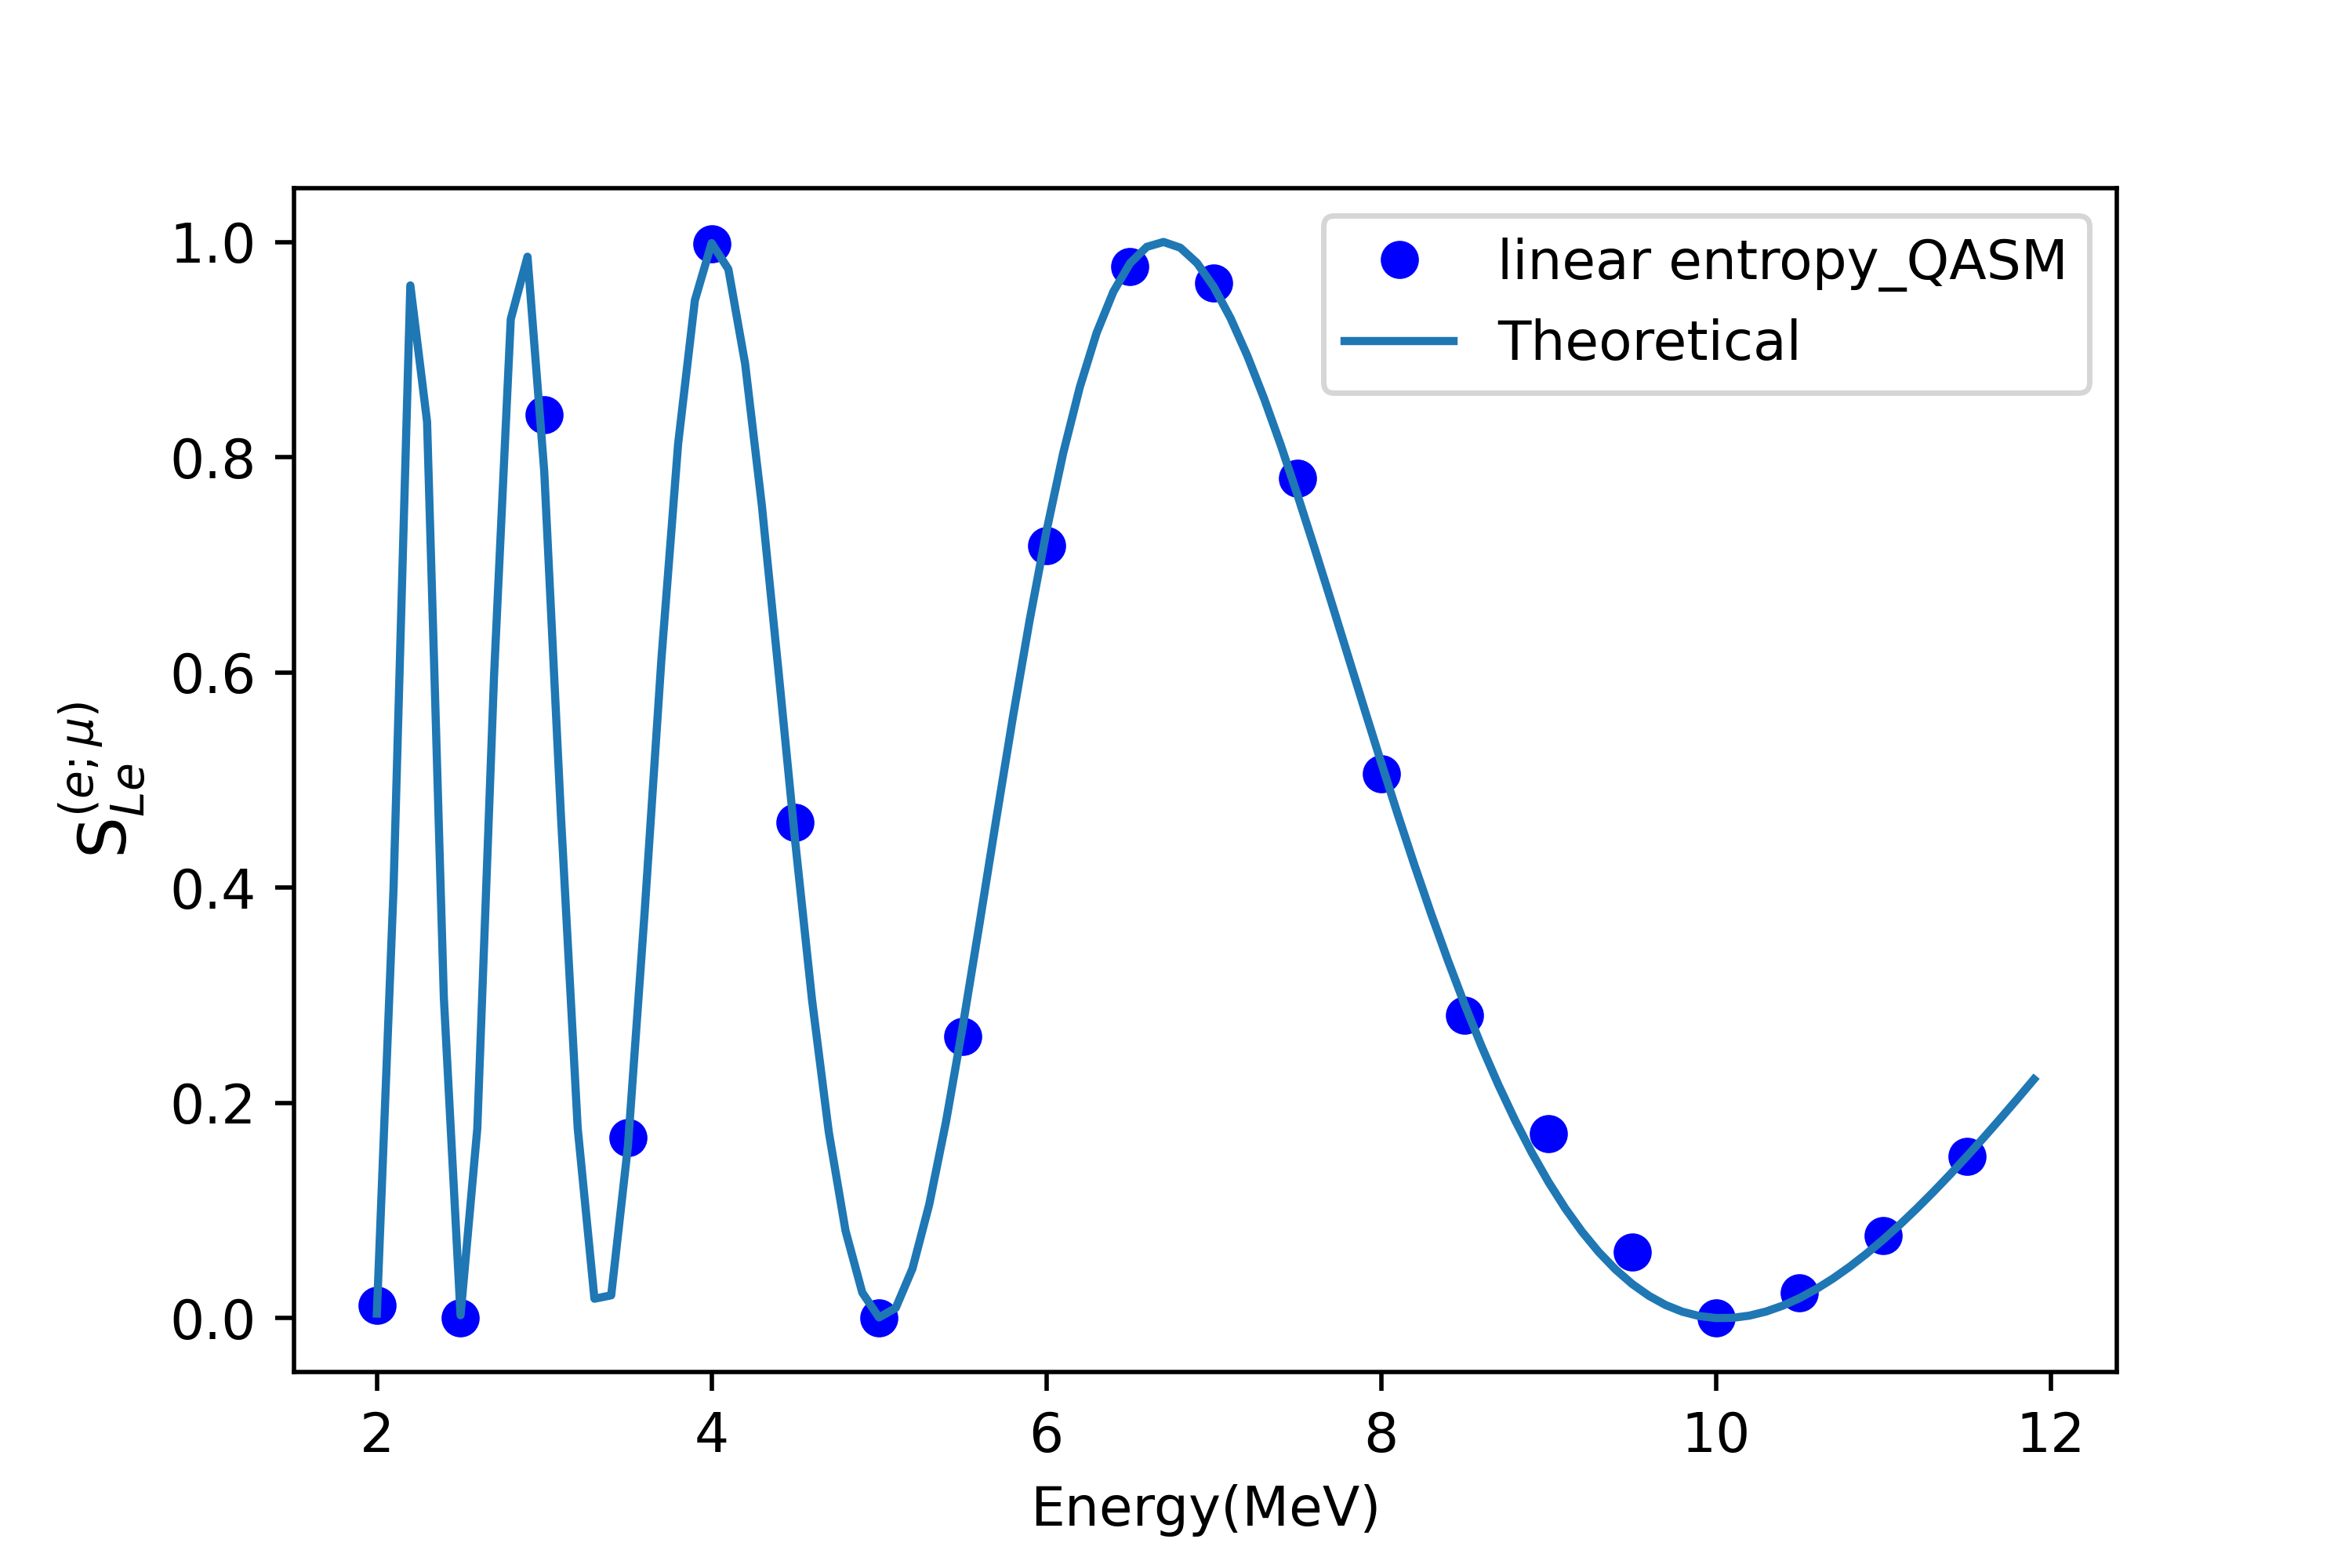
\includegraphics[width=0.8\textwidth]{fig_6a.png}}
	\caption{Linear entropy of $\nu_{e}-\nu_{\mu}$ system as a function of energy (in QASM simulator)}
	\label{fig 6a}
\end{figure}
\begin{figure}[H]
	\graphicspath{ {./Images/} }
	\centering	
	{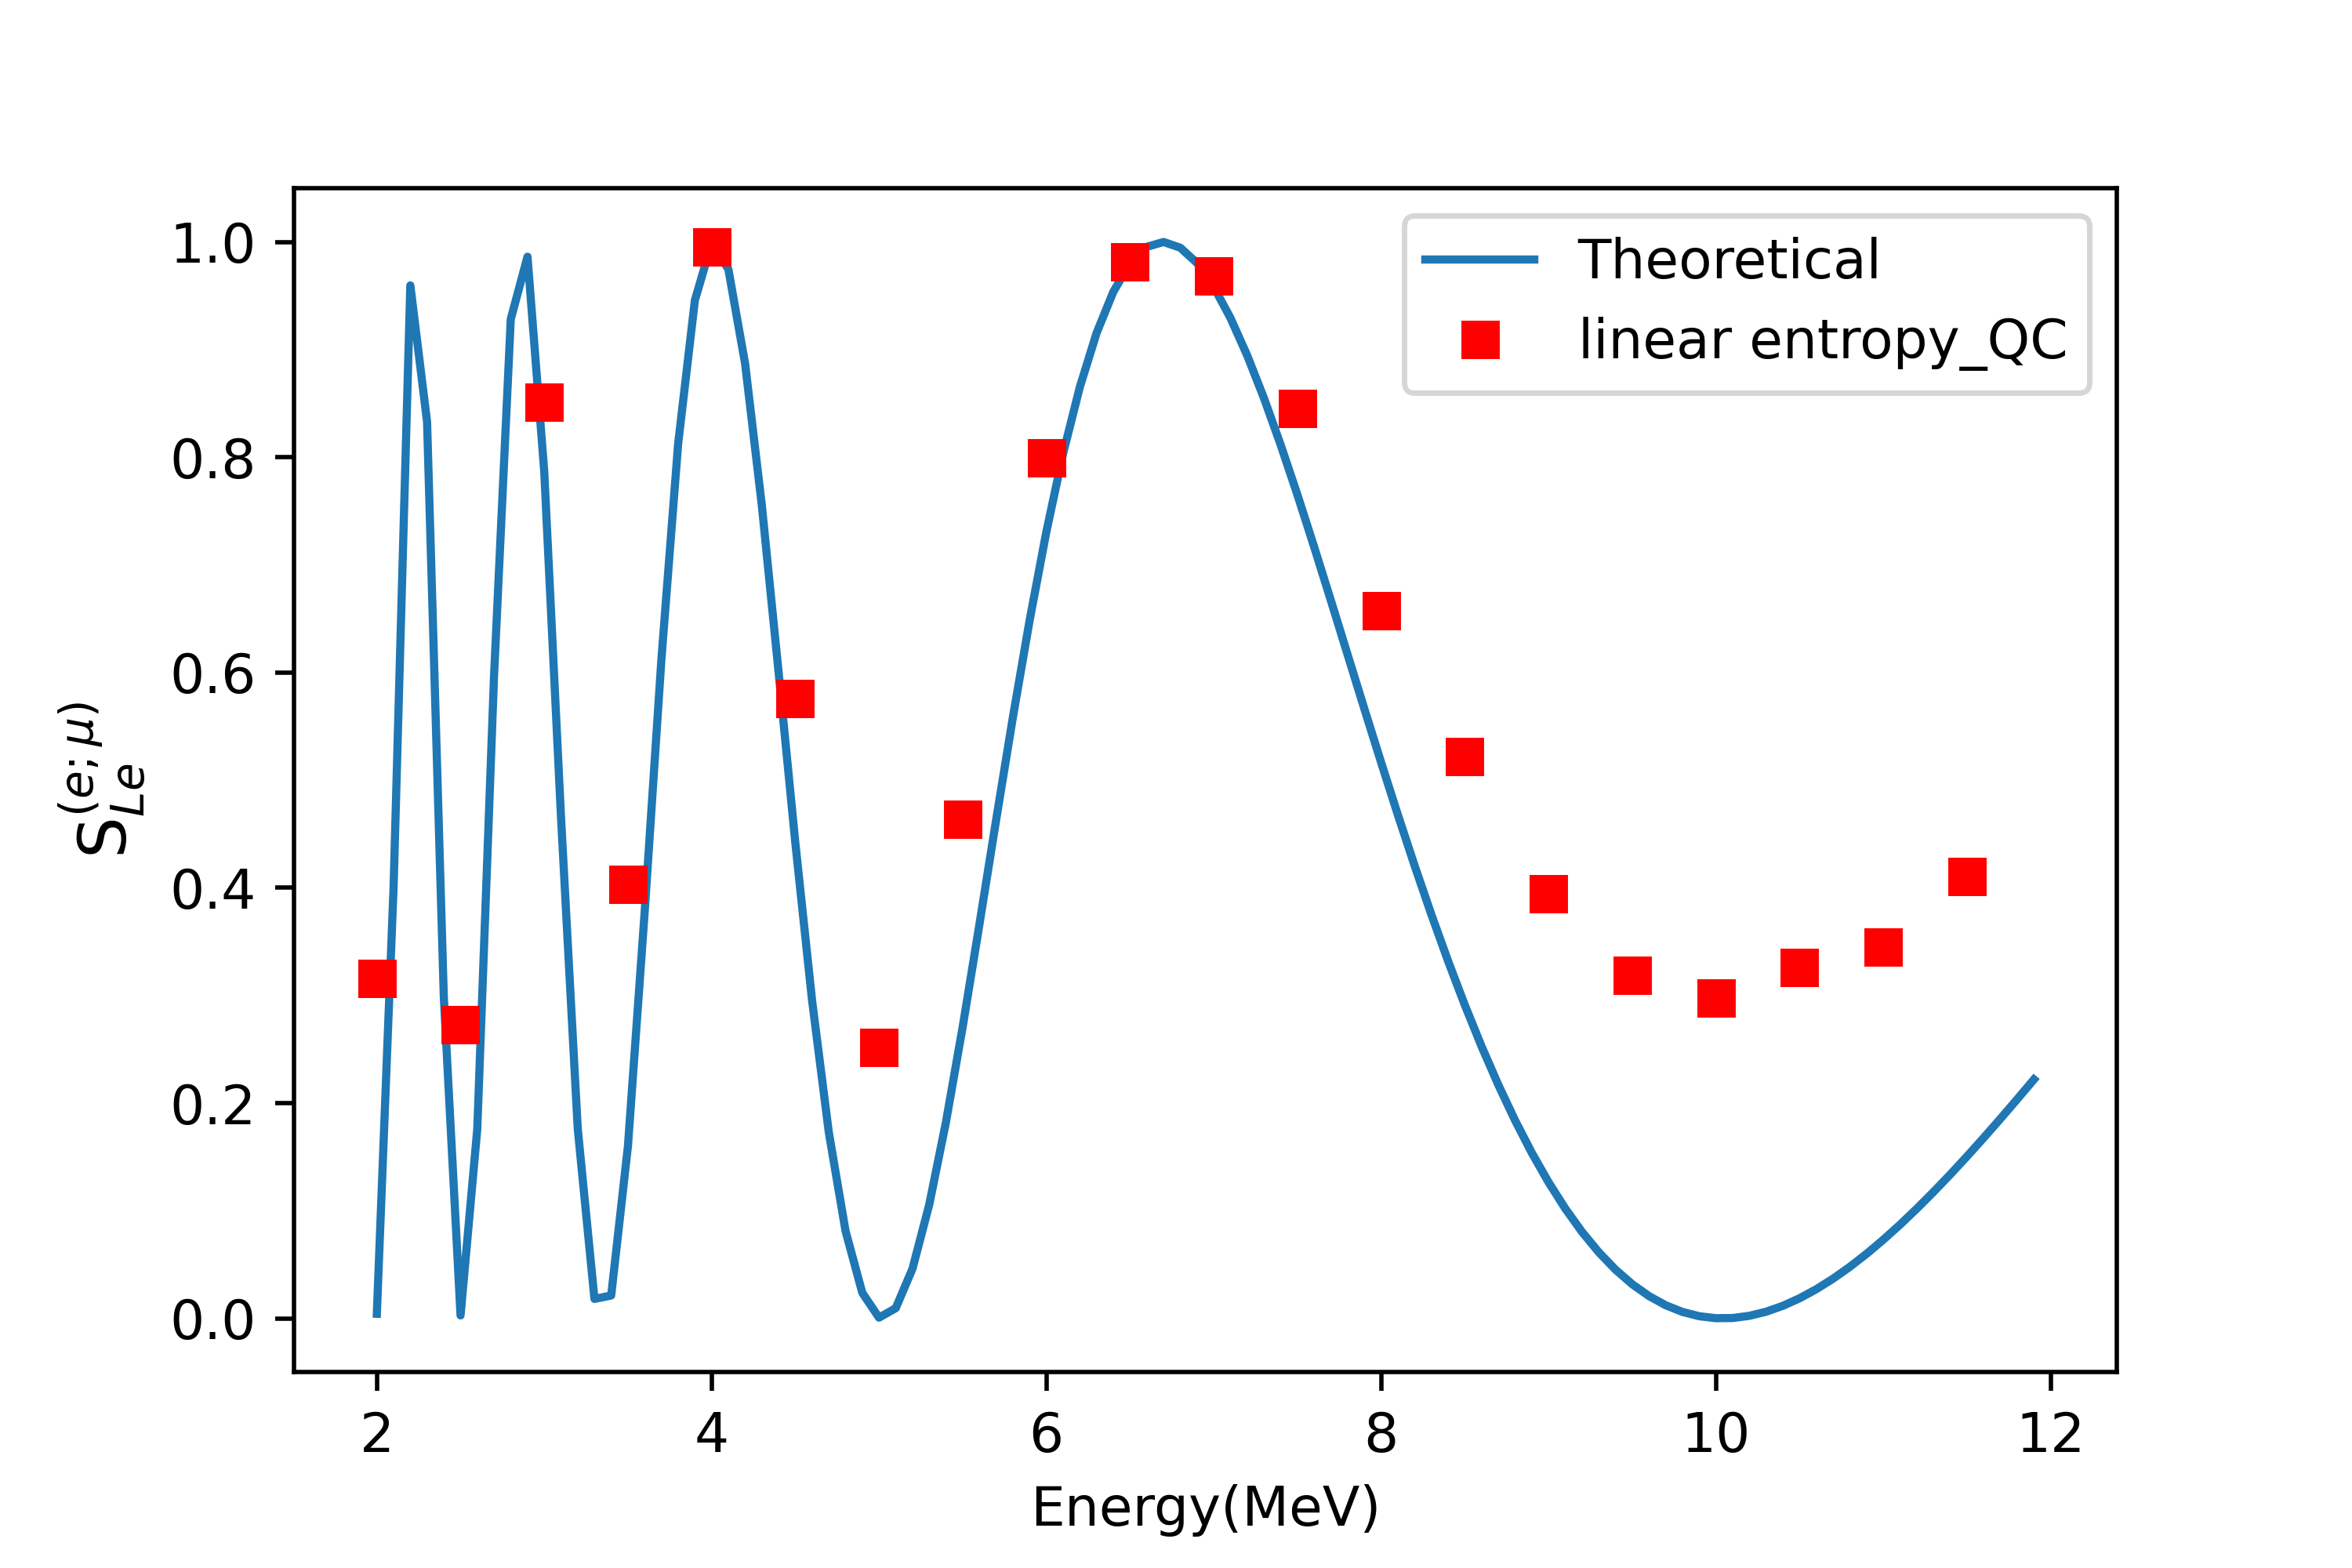
\includegraphics[width=0.8\textwidth]{fig_6b.png}}
	\caption{Linear entropy of $\nu_{e}-\nu_{\mu}$ system as a function of energy (in quantum computer)}
	\label{fig 6b}
\end{figure}
From figure $\ref{fig 6a}$, it is clear that circuit predicts the linear entropy accurately in the QASM simulator. Here also, the error happening while performing simulation on actual quantum computer is visible (figure $\ref{fig 6b}$). Linear entropy as discussed earlier is a monotone of entanglement. Thus can be used as direct measure of entanglement in the system. 
\begin{figure}[H]
	\graphicspath{ {./Images/} }
	\centering	
	{\includegraphics[width=0.8\textwidth]{fig_6a_1.png}}
	\caption{Entanglement in the $\nu_{e}-\nu_{\mu}$ system (in QASM simulator).}
	\label{fig 6a_1}
\end{figure}
\begin{figure}[H]
	\graphicspath{ {./Images/} }
	\centering	
	{\includegraphics[width=0.8\textwidth]{fig_6a_2.png}}
	\caption{Entanglement in the $\nu_{e}-\nu_{\mu}$ system (in Quantum computer).}
	\label{fig 6a_2}
\end{figure}
\pagebreak
Here $T=\frac{\Delta m^{2}t}{2E\hbar}$. If we fix the value of $E$, then $T$ soley depends upon time $t$. At $T=0$, the disappearance probability ($P_{\nu_{\mu}\rightarrow\nu_{\mu}}$) is maximum and appearance probability ($P_{\nu_{\mu}\rightarrow\nu_{e}}$) is minimum. Thus system will have least entropy. As a result system will have the least entanglement. In our case, system behaves like a product state at $T=0$. As time evolves (T increases), neutrinos began to undergo flavour oscillation. Appearance and disappearance probabilities show sinusoidal nature with time. Thus the linear entropy of the system varies in sinusoidal manner. Linear entropy is maximum when $P_{\nu_{\mu}\rightarrow\nu_{\mu}}=P_{\nu_{\mu}\rightarrow\nu_{e}}=0.5$. Therefore, system will be maximally entangled at this value of $T$ and minimum at $T=\pi$. This behaviour is clearly demonstrated in figures $\ref{fig 6a_1}$ and $\ref{fig 6a_2}$. Even though quantum computer gives the behaviour of system, it does not accurately the measure of entanglement.
\section{Three Flavour Oscillation: Simulation Results}
To perform three flavour oscillation, we used the circuit given in the figure $\ref{fig 4}$. We studied a system where all the neutrinos were of muon flavour initially. Through simulation we conducted appearance and disappearance experiments.
\begin{figure}[H]
\graphicspath{ {./Images/} }
\centering	
{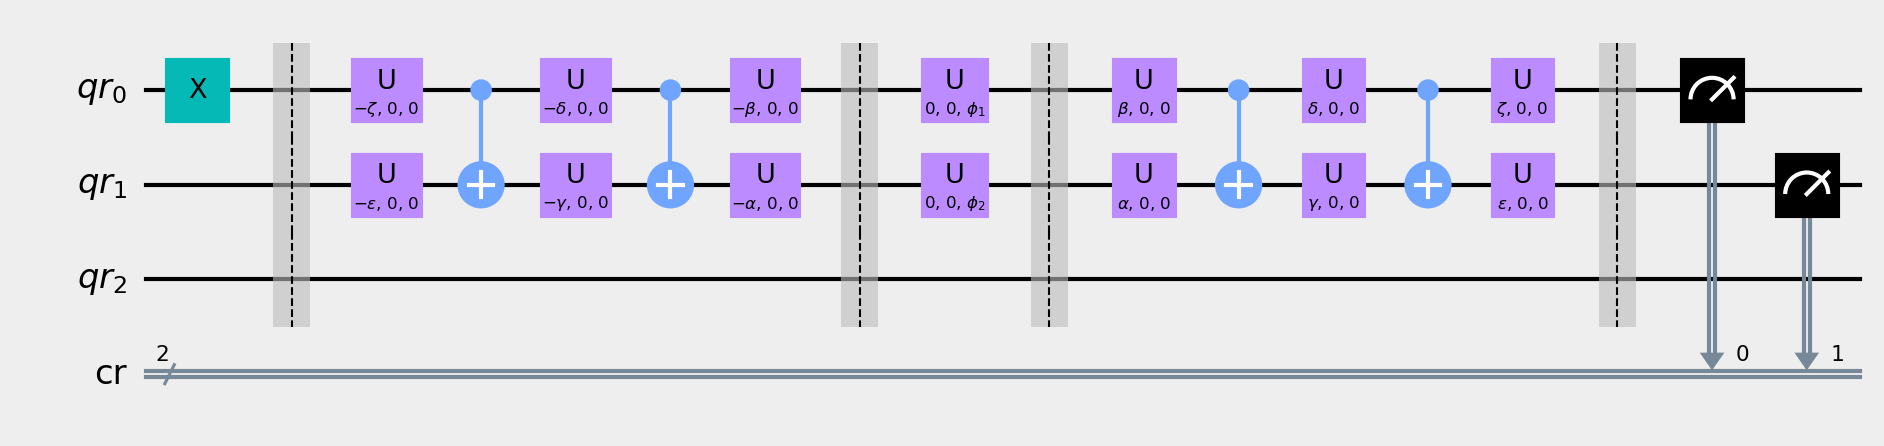
\includegraphics[width=\textwidth]{fig_7.png}}
\end{figure}\par
Here we prepare muon neutrino using the encoding scheme discussed earlier (equation $\ref{eq:17}$),and then time evolved it. The output state is projected in to the basis $\{\ket{00},\ket{01},\ket{10},\ket{11}\}$. We run the circuit 1024 times.  Count of $\ket{10}$ state gives disappearance count of muon neutrino. Count of $\ket{01}$ and $\ket{00}$ gives the appearance count of tau and electron neutrino respectively. From these counts we can calculate corresponding probabilities.

Parameters required for simulation (mixing angle and mass square splittings) are taken from \cite{estaban}.  Simulations were performed on both the QASM simulator and the IBM Quantum computer.
\subsection{Simulation Using QASM Simulator}
\begin{figure}[H]
	\graphicspath{ {./Images/} }	
	{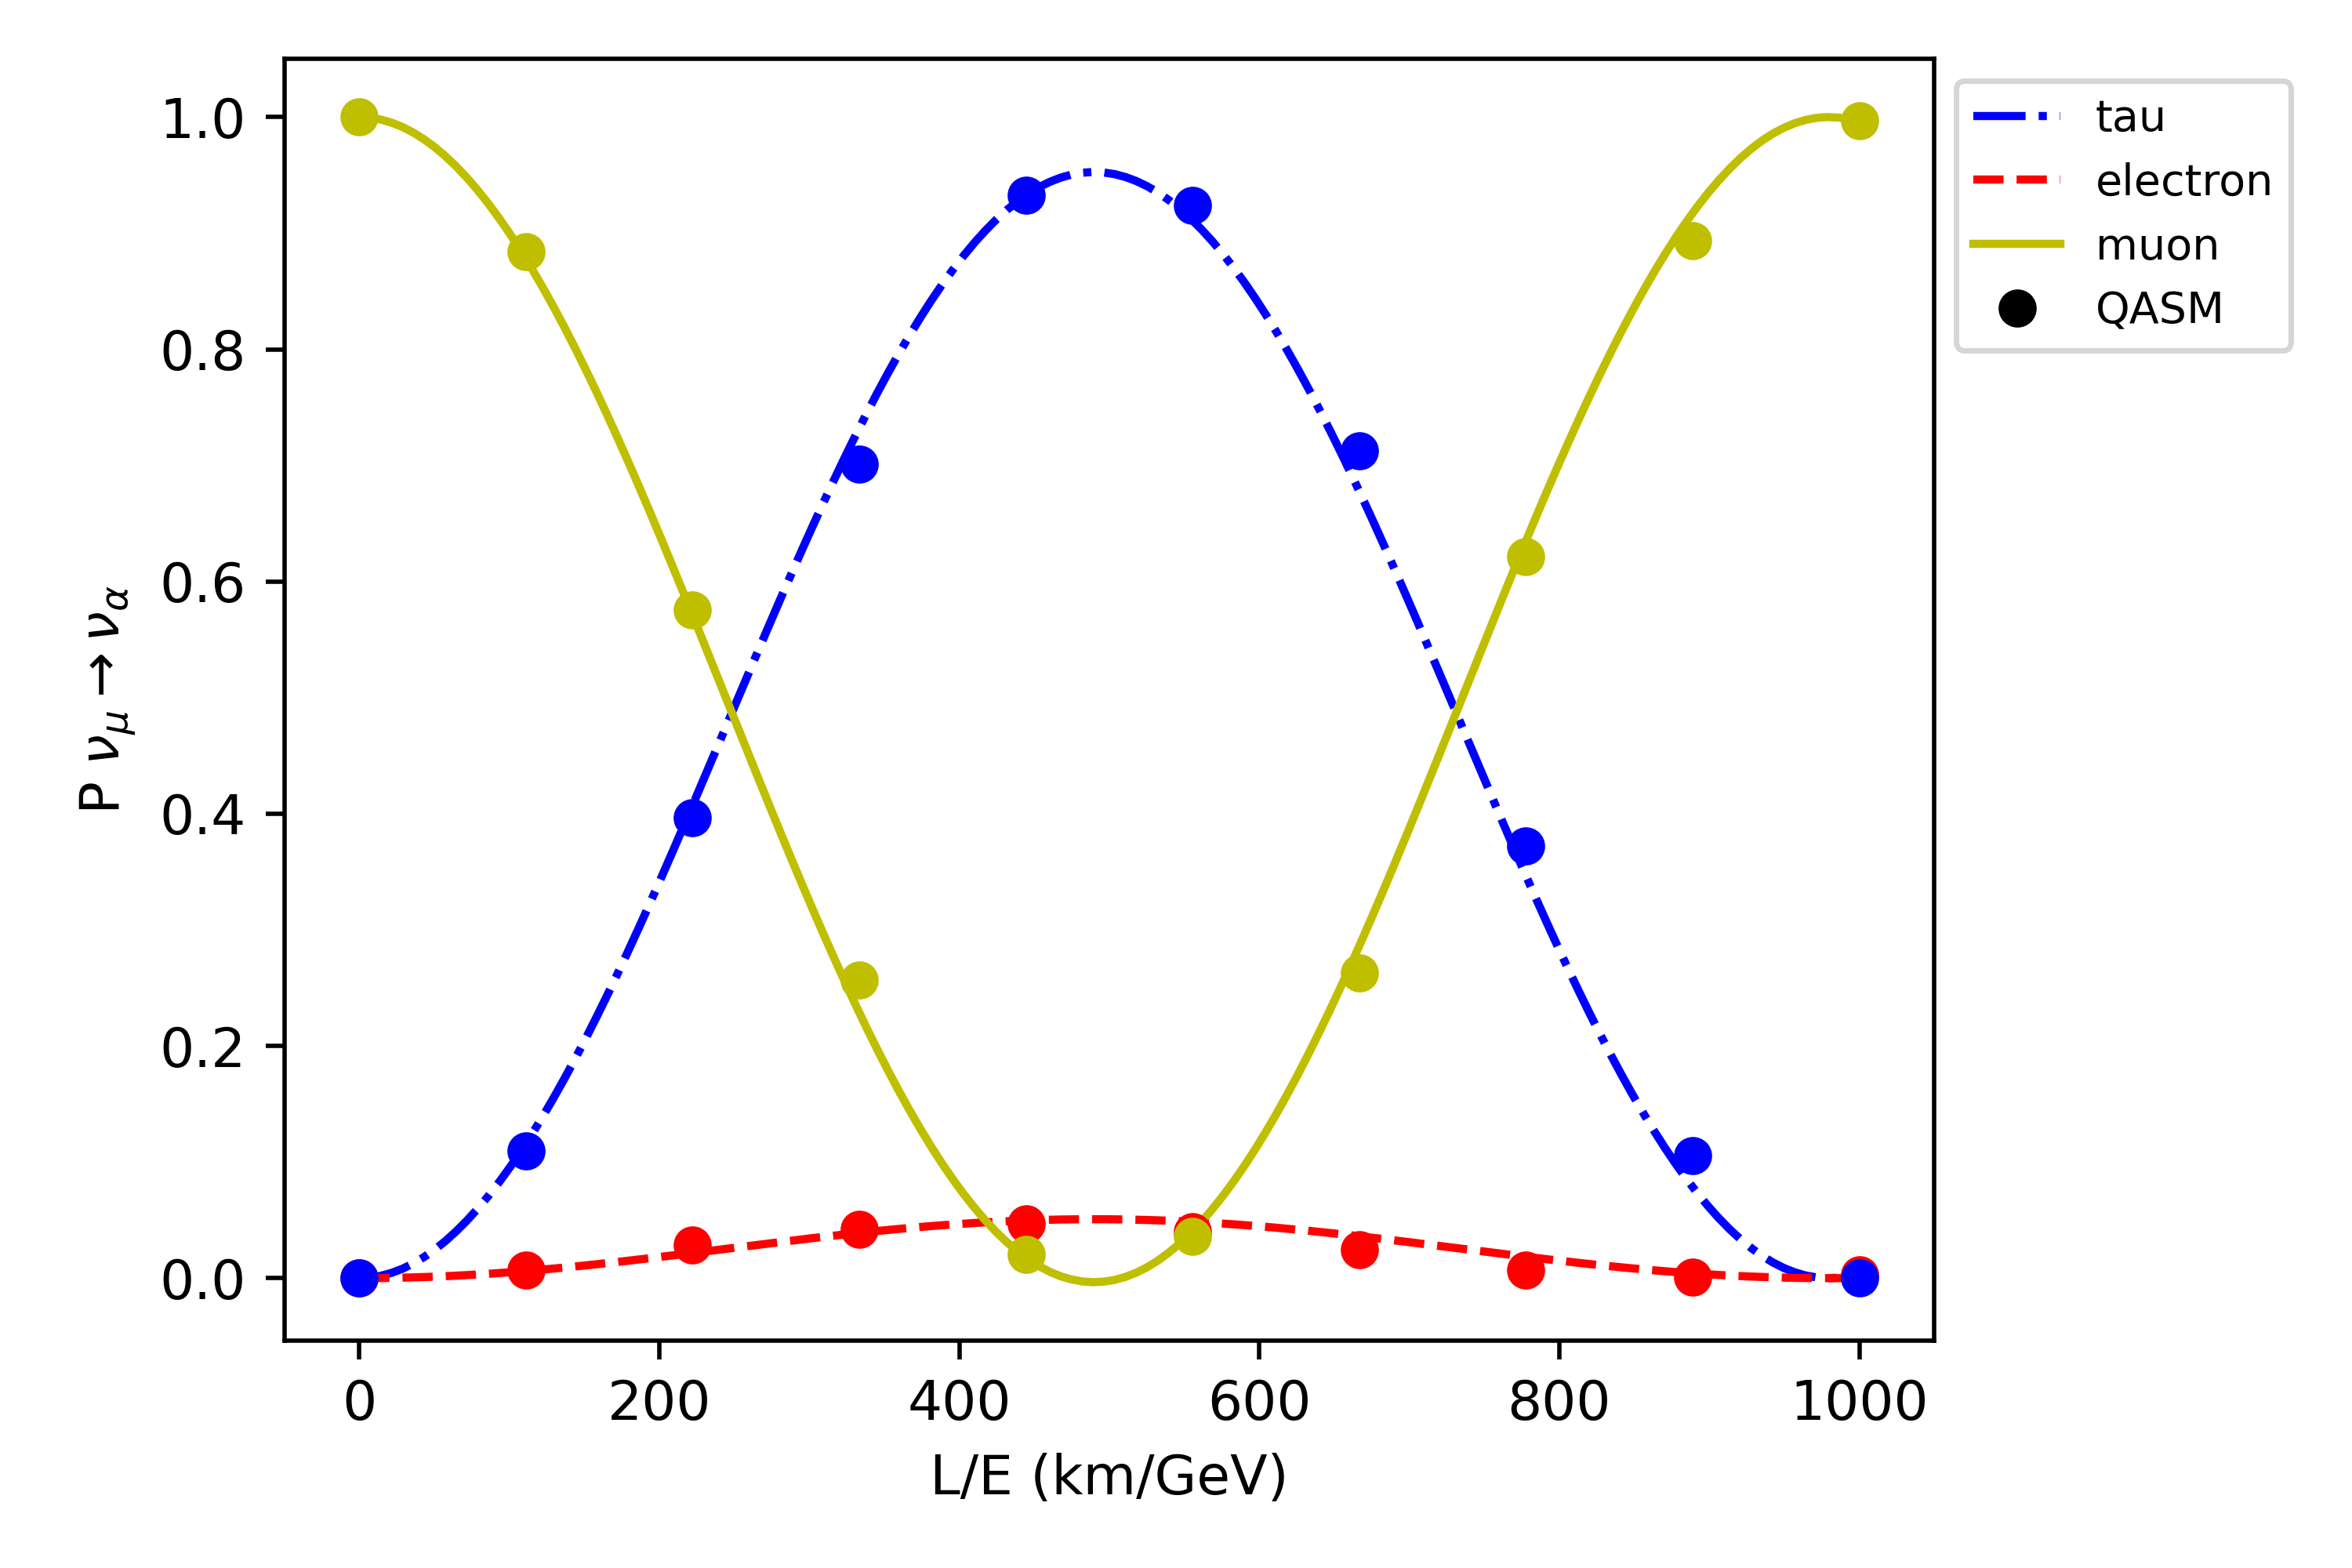
\includegraphics[scale=0.8]{fig_8.png}}
	\centering\caption{ Three flavour oscillation probability as function of time (in QASM simulator)}
		\label{fig 8}
	\end{figure}
Here in the $Y$ axis we plot probability of transition from a muon flavour to a particular flavour $\alpha$. It should be noted that alpha could be any flavour ($\alpha=e,\mu,\tau$). We calculated disappearance probability of muon and appearance probability of electron and tau for various values $\frac{L}{E}$ with each experiment composed of 1024 trials. The plot showing how probabilities vary with $\frac{L}{E}$ is plotted.
	From the figure $\ref{fig 8}$ it is clear that circuit works fine even though there are slight deviations can from theoretical value.
\subsection{Simulation Using IBM Quantum Computer}
The circuit was run on IBM Quantum computer named IBM Lima. It is a five qubit system.\\

\begin{minipage}{0.5\textwidth}
\textbf{IBM Lima}\\	
Quantum Volume : 8 \\
Processor: Falcon r4\\
Basis gates: CX, ID, RZ, SX, X\\
\end{minipage}%
\begin{minipage}{0.5\textwidth}
Avg. CNOT Error: 1.220e-2\\
Avg. Readout Error: 3.860e-2\\
Avg. T1: 76.74 $\mu$s\\
Avg. T2: 73.74 $\mu$s\\

\end{minipage}

We performed 1024 trails. We qot back appearance and disappearance counts. Oscillation probabilities were founded from these counts and experiment was repeated for different $\frac{L}{E}$ values.
\begin{figure}[h]
	\graphicspath{ {./Images/} }
	\centering	 predicted by the circuit from the actual value. As discussed above, the err
	{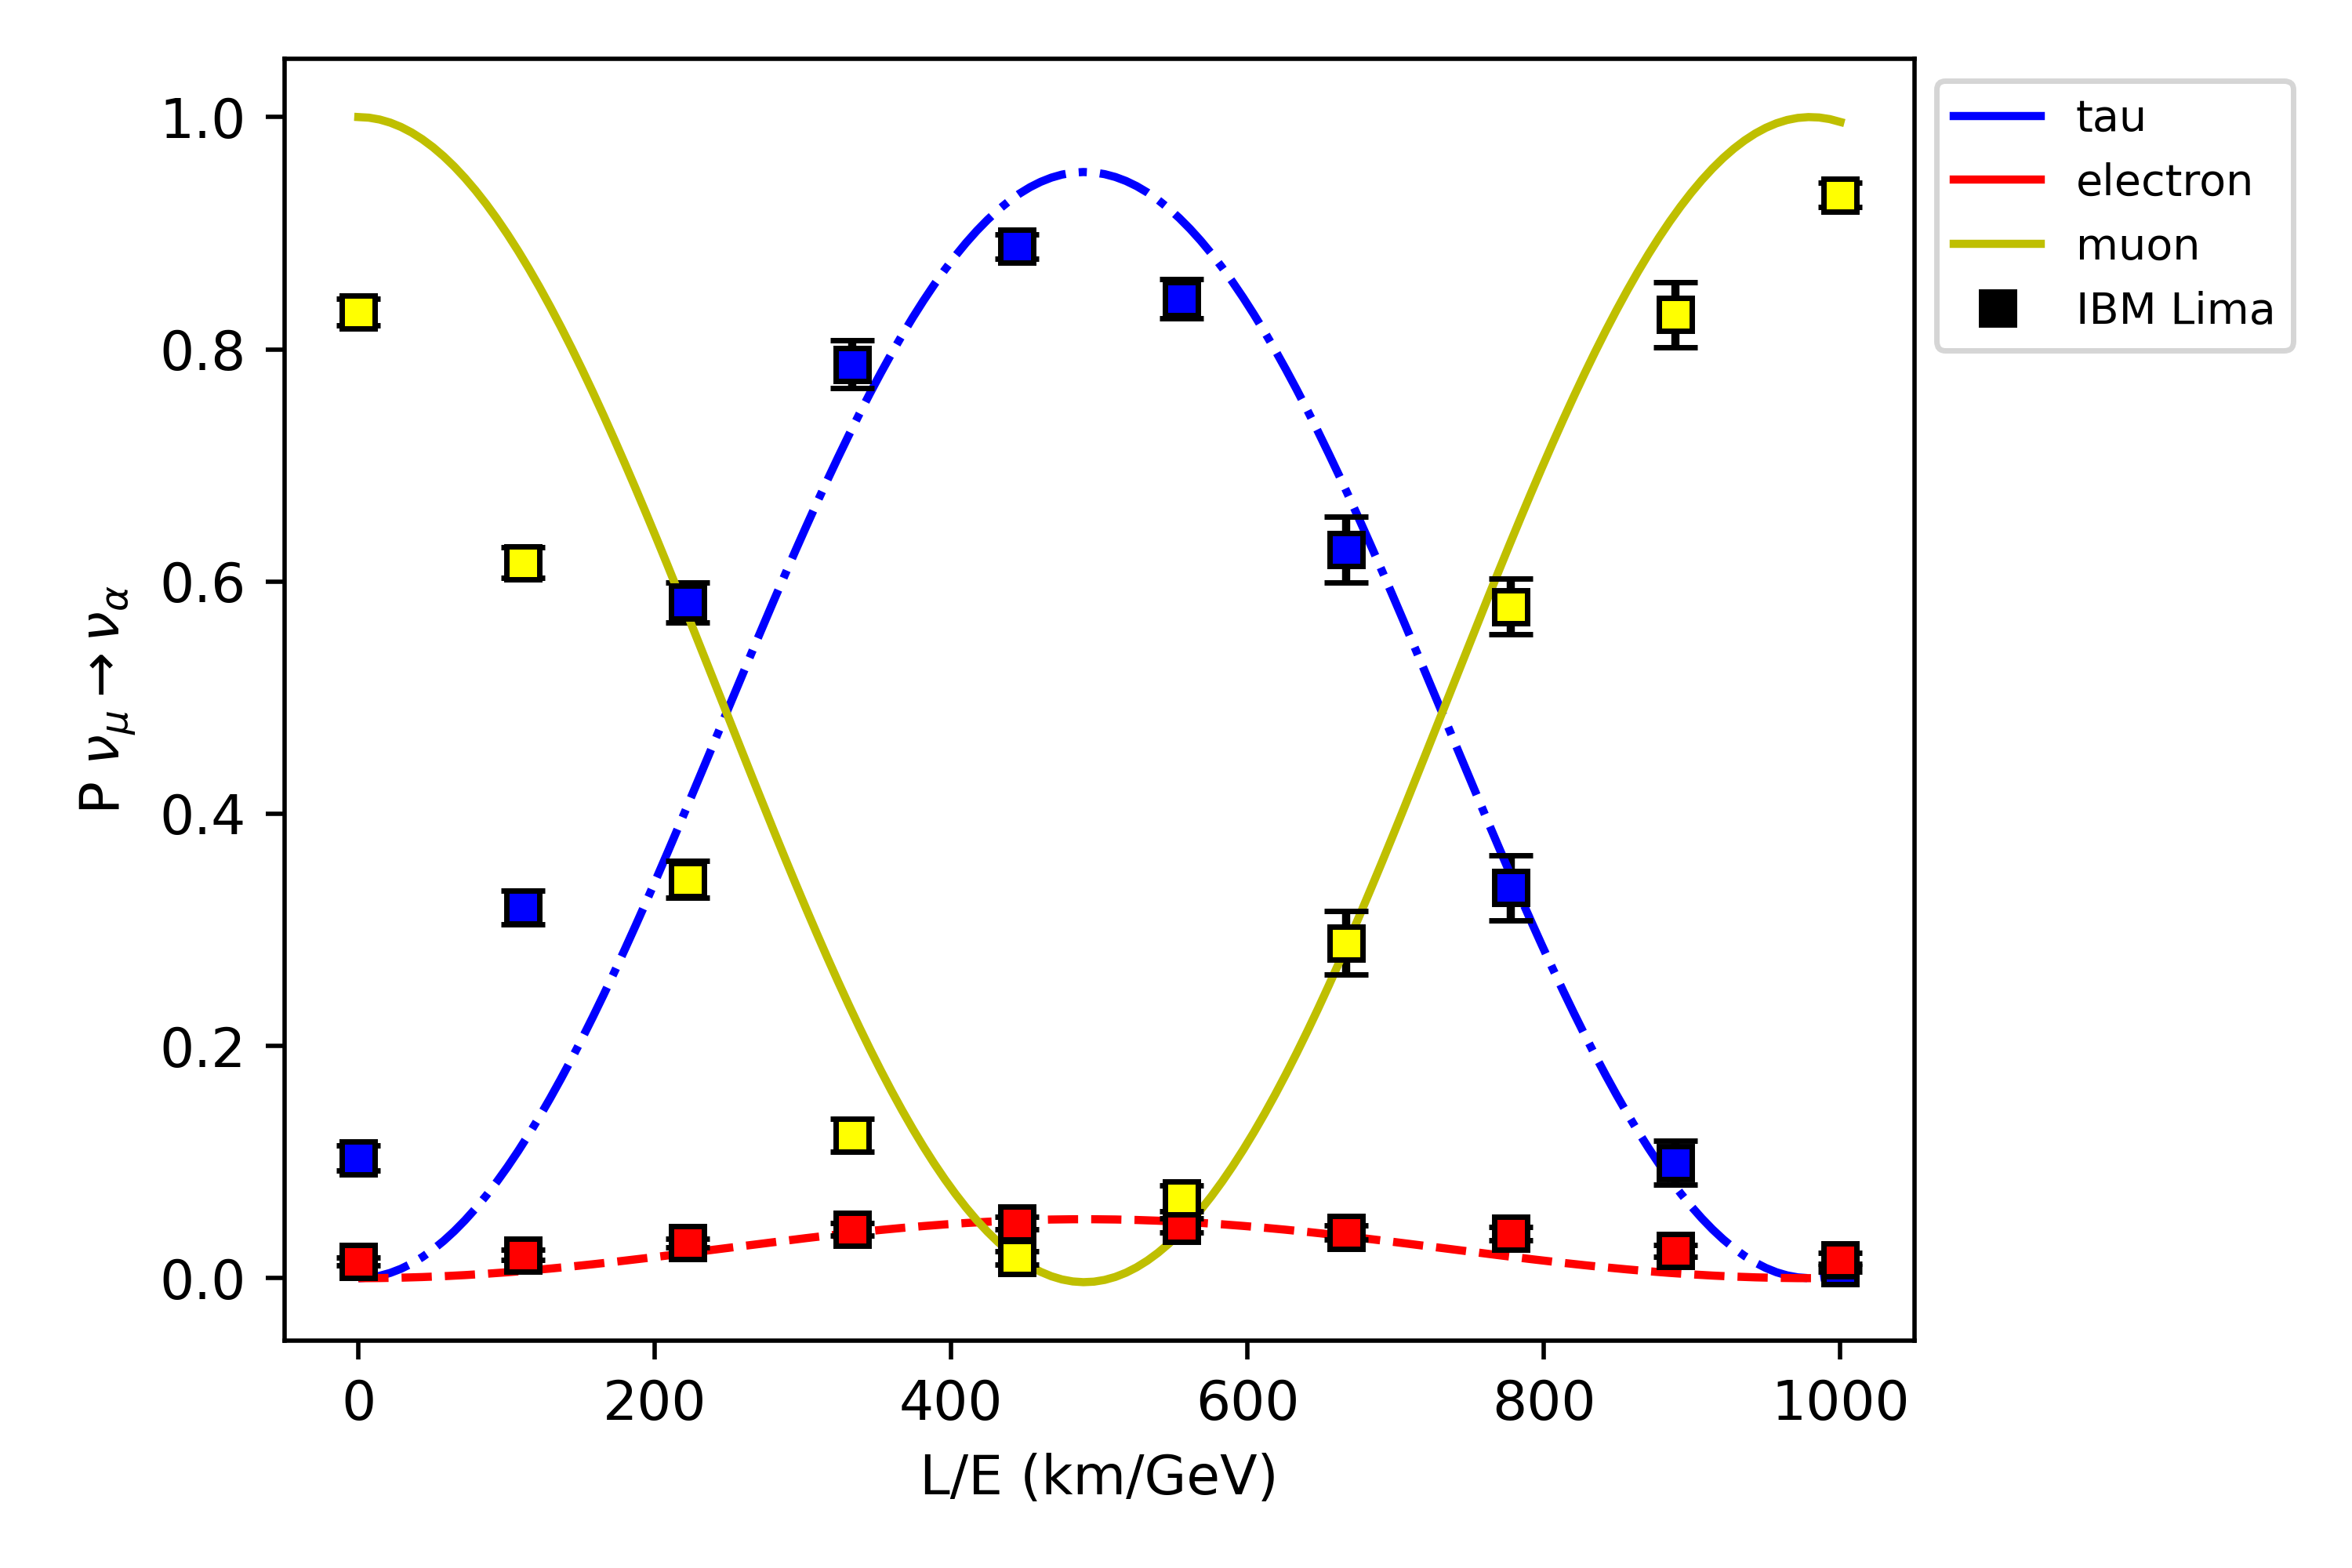
\includegraphics[scale=0.8]{fig_9.png}}
	\caption{Three flavour oscillation probability as function of time (in Quantum computer) }
		\label{fig 9}
	\end{figure}\par
	Here we also have accounted for the statistical error that may happen while running circuits on actual quantum computers. For a particular value of $\frac{L}{E}$, we repeated the experiment 10 times and calculated standard deviations of data. \par 
	One can see deviations of oscillation probabilities predicted by the circuit from the actual value. As discussed above, the errors are due to large length of the circuit. Compared to two flavour case, number of single qubit gates used is 5 times large and each gate approximately induce an error of $\mathcal{O}(0.1\%)$ .This circuit also uses 4 two qubit gates which also induce errors into results. Further readout errors  ($\mathcal{O}(5\%)$ can also influence final results. Also, due to $T_{1}$ and $T_{2}$ errore $\ket{11}$ have non zero counts in quantum computers. This affect the appearance and disappearance probabilities.
\subsection{Entanglement Studies}
Through simulation using the circuit in figure $\ref{fig 4}$, we can get the disappearance and appearance probabilities in a three flavour system. We can use this data to find out the linear entropy.
\begin{figure}[H]
	\graphicspath{ {./Images/} }
	\centering	
	{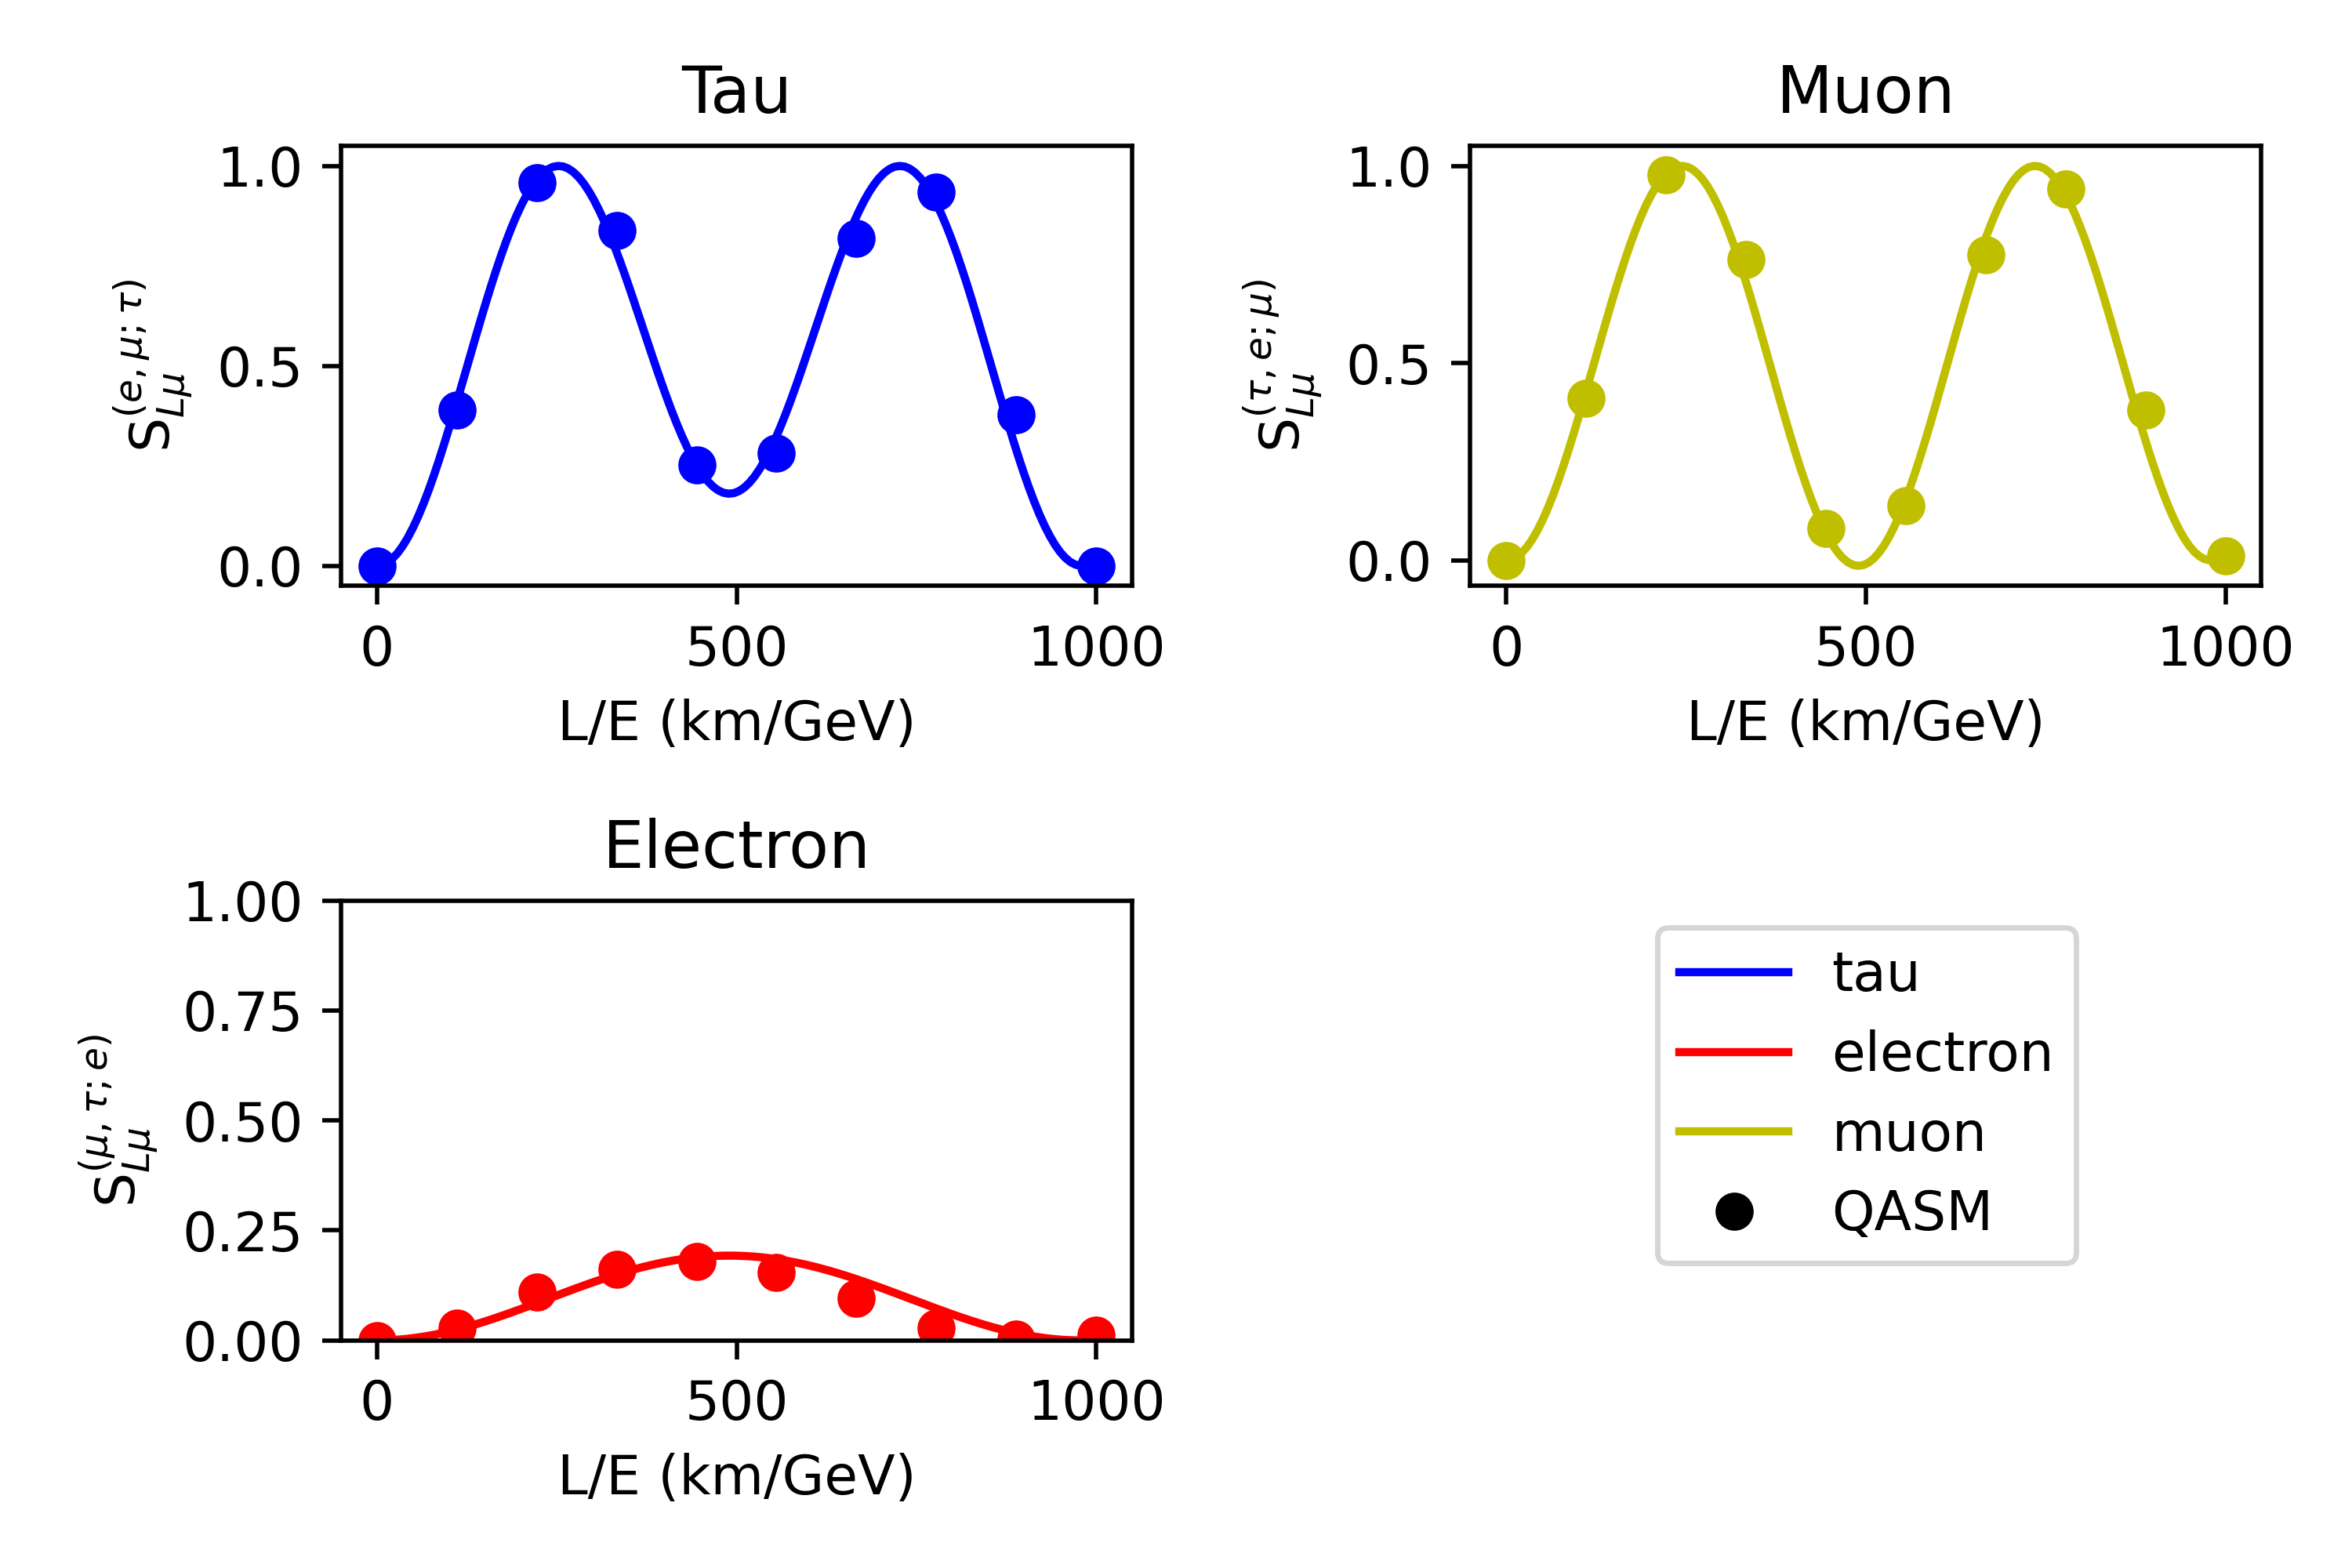
\includegraphics[width=0.8\textwidth]{fig_9a.png}}
	\caption{Linear entropy of 3-flavour system as a function of energy (in QASM simulator)}
	\label{fig 9a}
\end{figure}
\begin{figure}[H]
	\graphicspath{ {./Images/} }
	\centering	
	{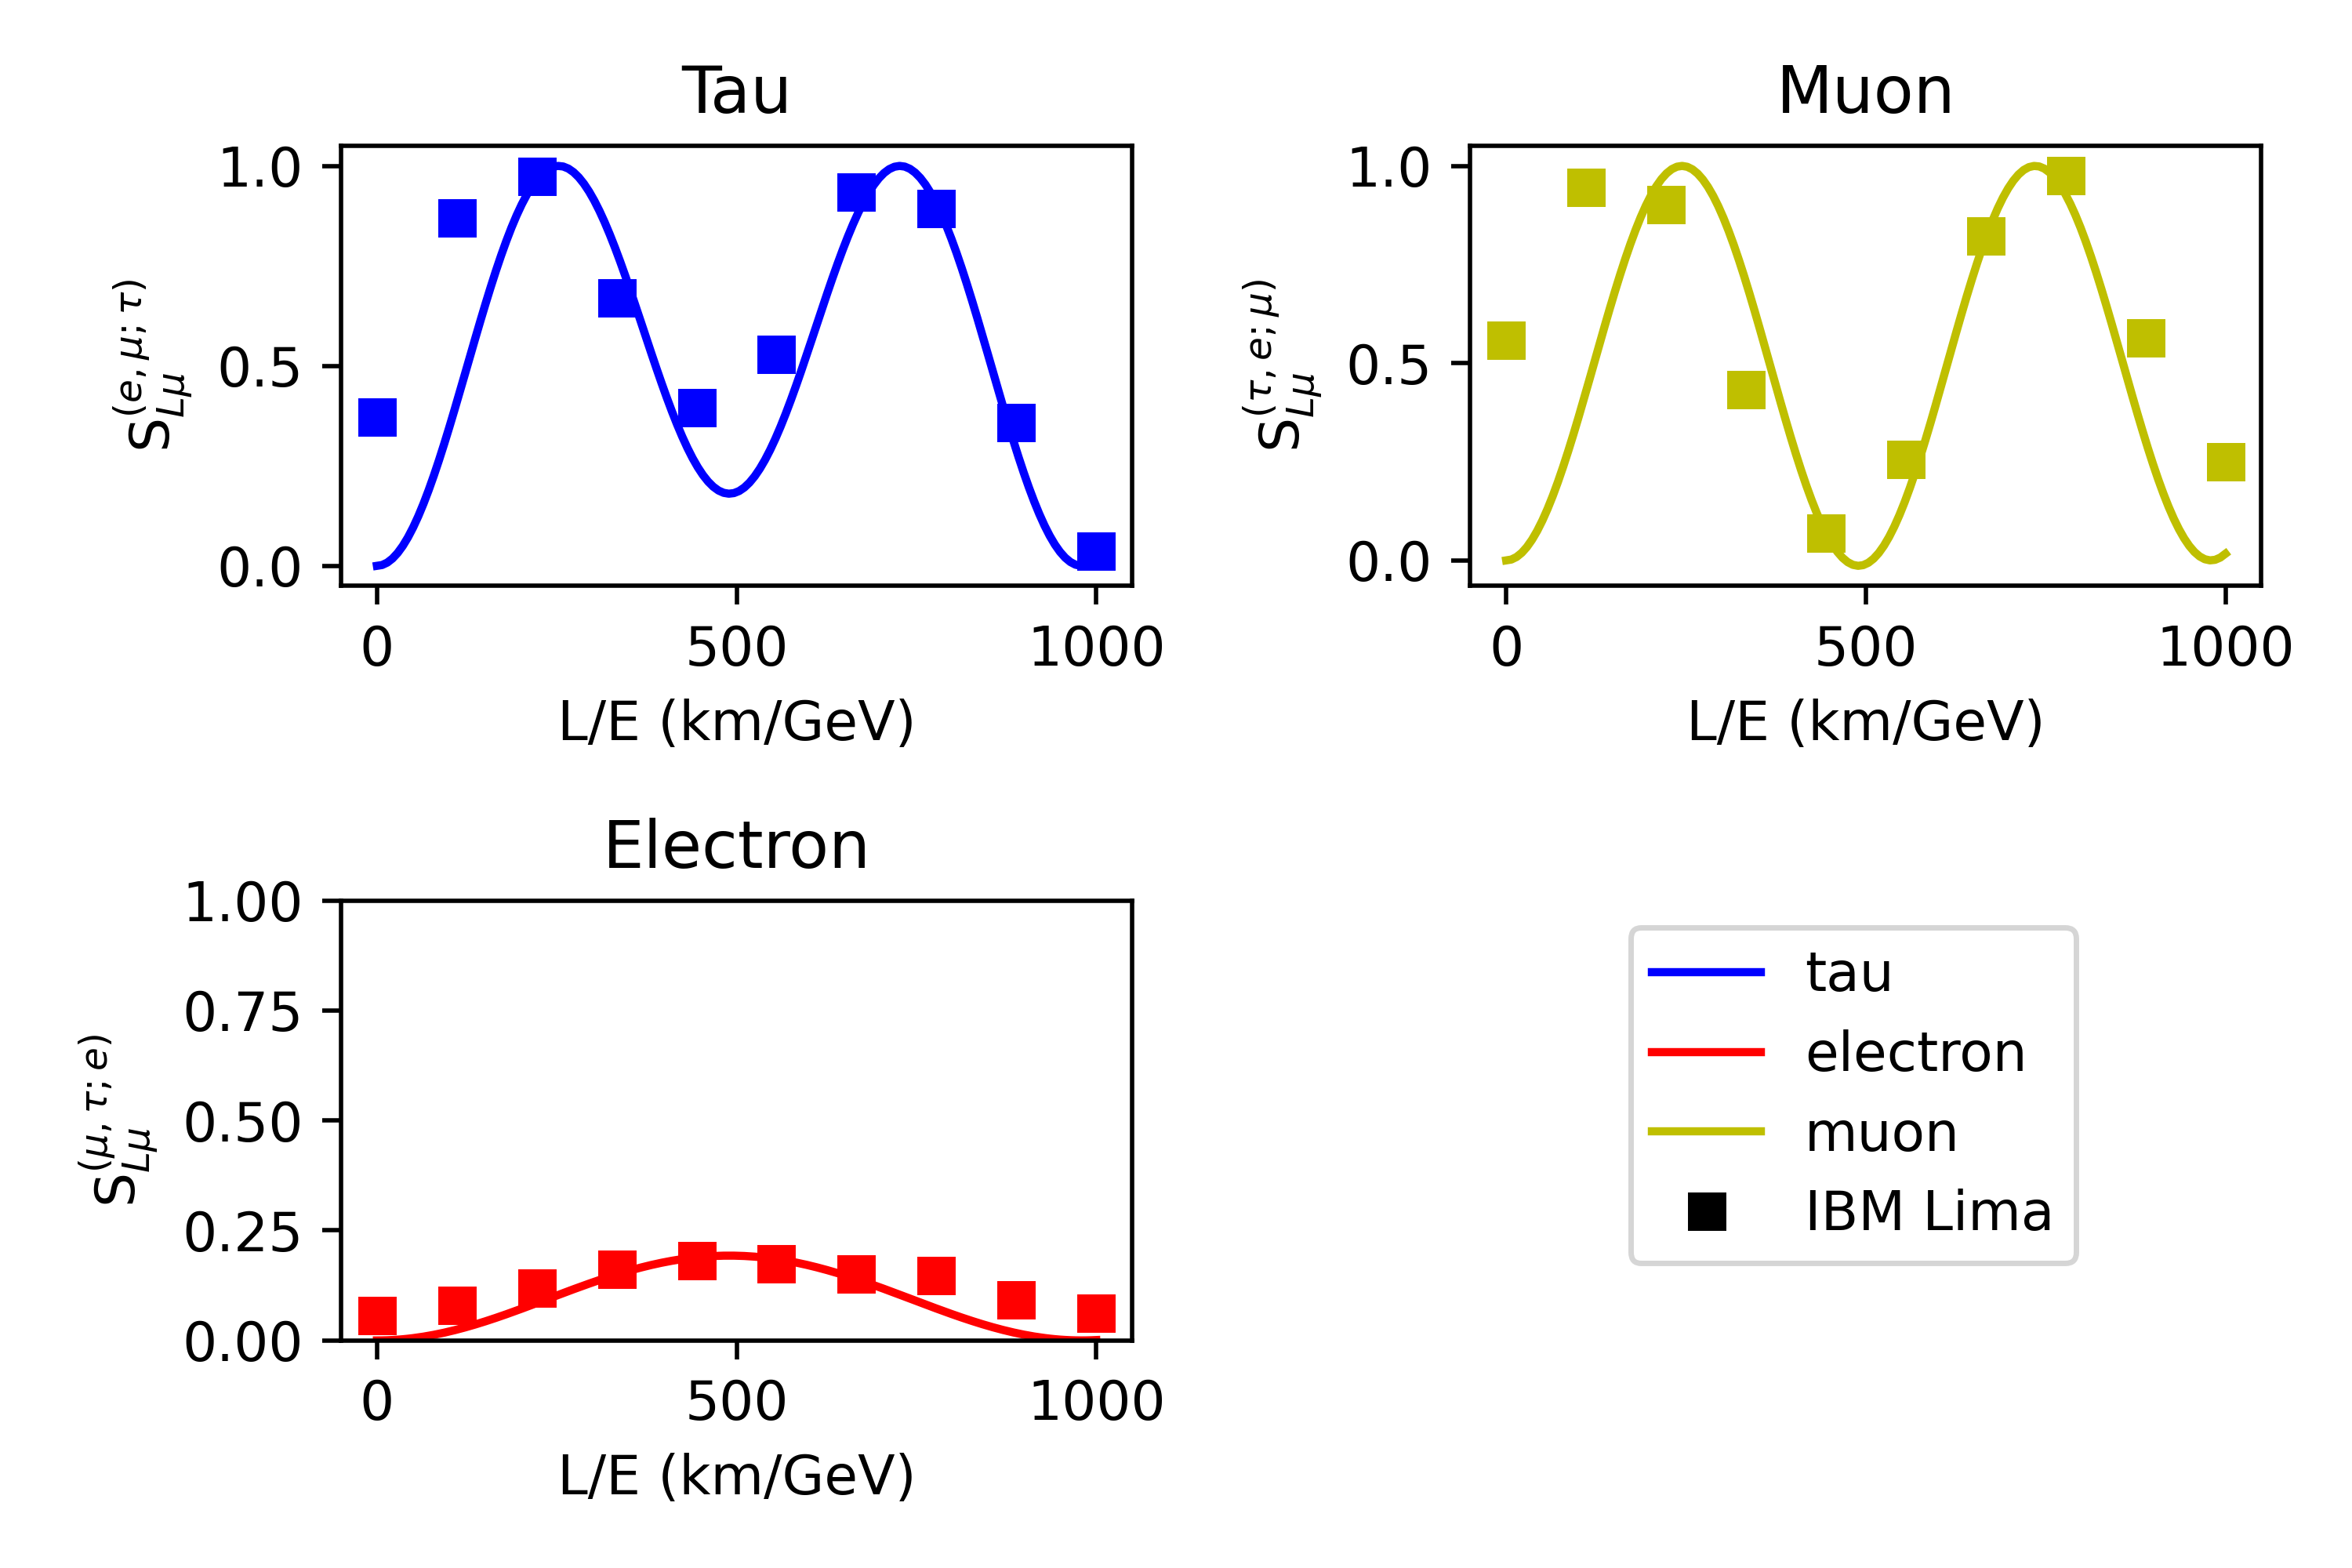
\includegraphics[width=0.8\textwidth]{fig_9b.png}}
	\caption{Linear entropy of 3-flavour system as a function of energy (in quantum computer)}
	\label{fig 9b}
\end{figure}

In the figure $\ref{fig 9a}$, the first subplot represent $e\mu-\tau$ system. We partition the system into two subsystem. One composed of electron-muon flavour and other composed of tau flavour. This is done by tracing out tau flavour from the density matrix. Thus using the reduced density matrix of tau, we find out linear entropy the total system ($S^{(e,\mu;\tau)}_{L\mu}$). Similarly, second and third subplots give linear entropy of the systems after tracing out muon ($S^{(\tau,e;\mu)}_{L\mu}$) and electron neutrino ($S^{(\mu,\tau;e)}_{L\mu}$)respectively.
The circuit predicts the linear entropy with reasonable accurately in the QASM simulator. But while performing simulation on actual quantum computer error arises (figure $\ref{fig 9b}$). Using the linear entropy, we can calaculate the average linear entropy of total system. This act as a measure of global entanglement in the system. 
\begin{figure}[H]
	\graphicspath{ {./Images/} }
	\centering	
	{\includegraphics[width=0.8\textwidth]{fig_9a_1.png}}
	\caption{Global entanglement in the 3-flavour system (in QASM simulator).}
	\label{fig 9a_1}
\end{figure}
\begin{figure}[h]
	\graphicspath{ {./Images/} }
	\centering	
	{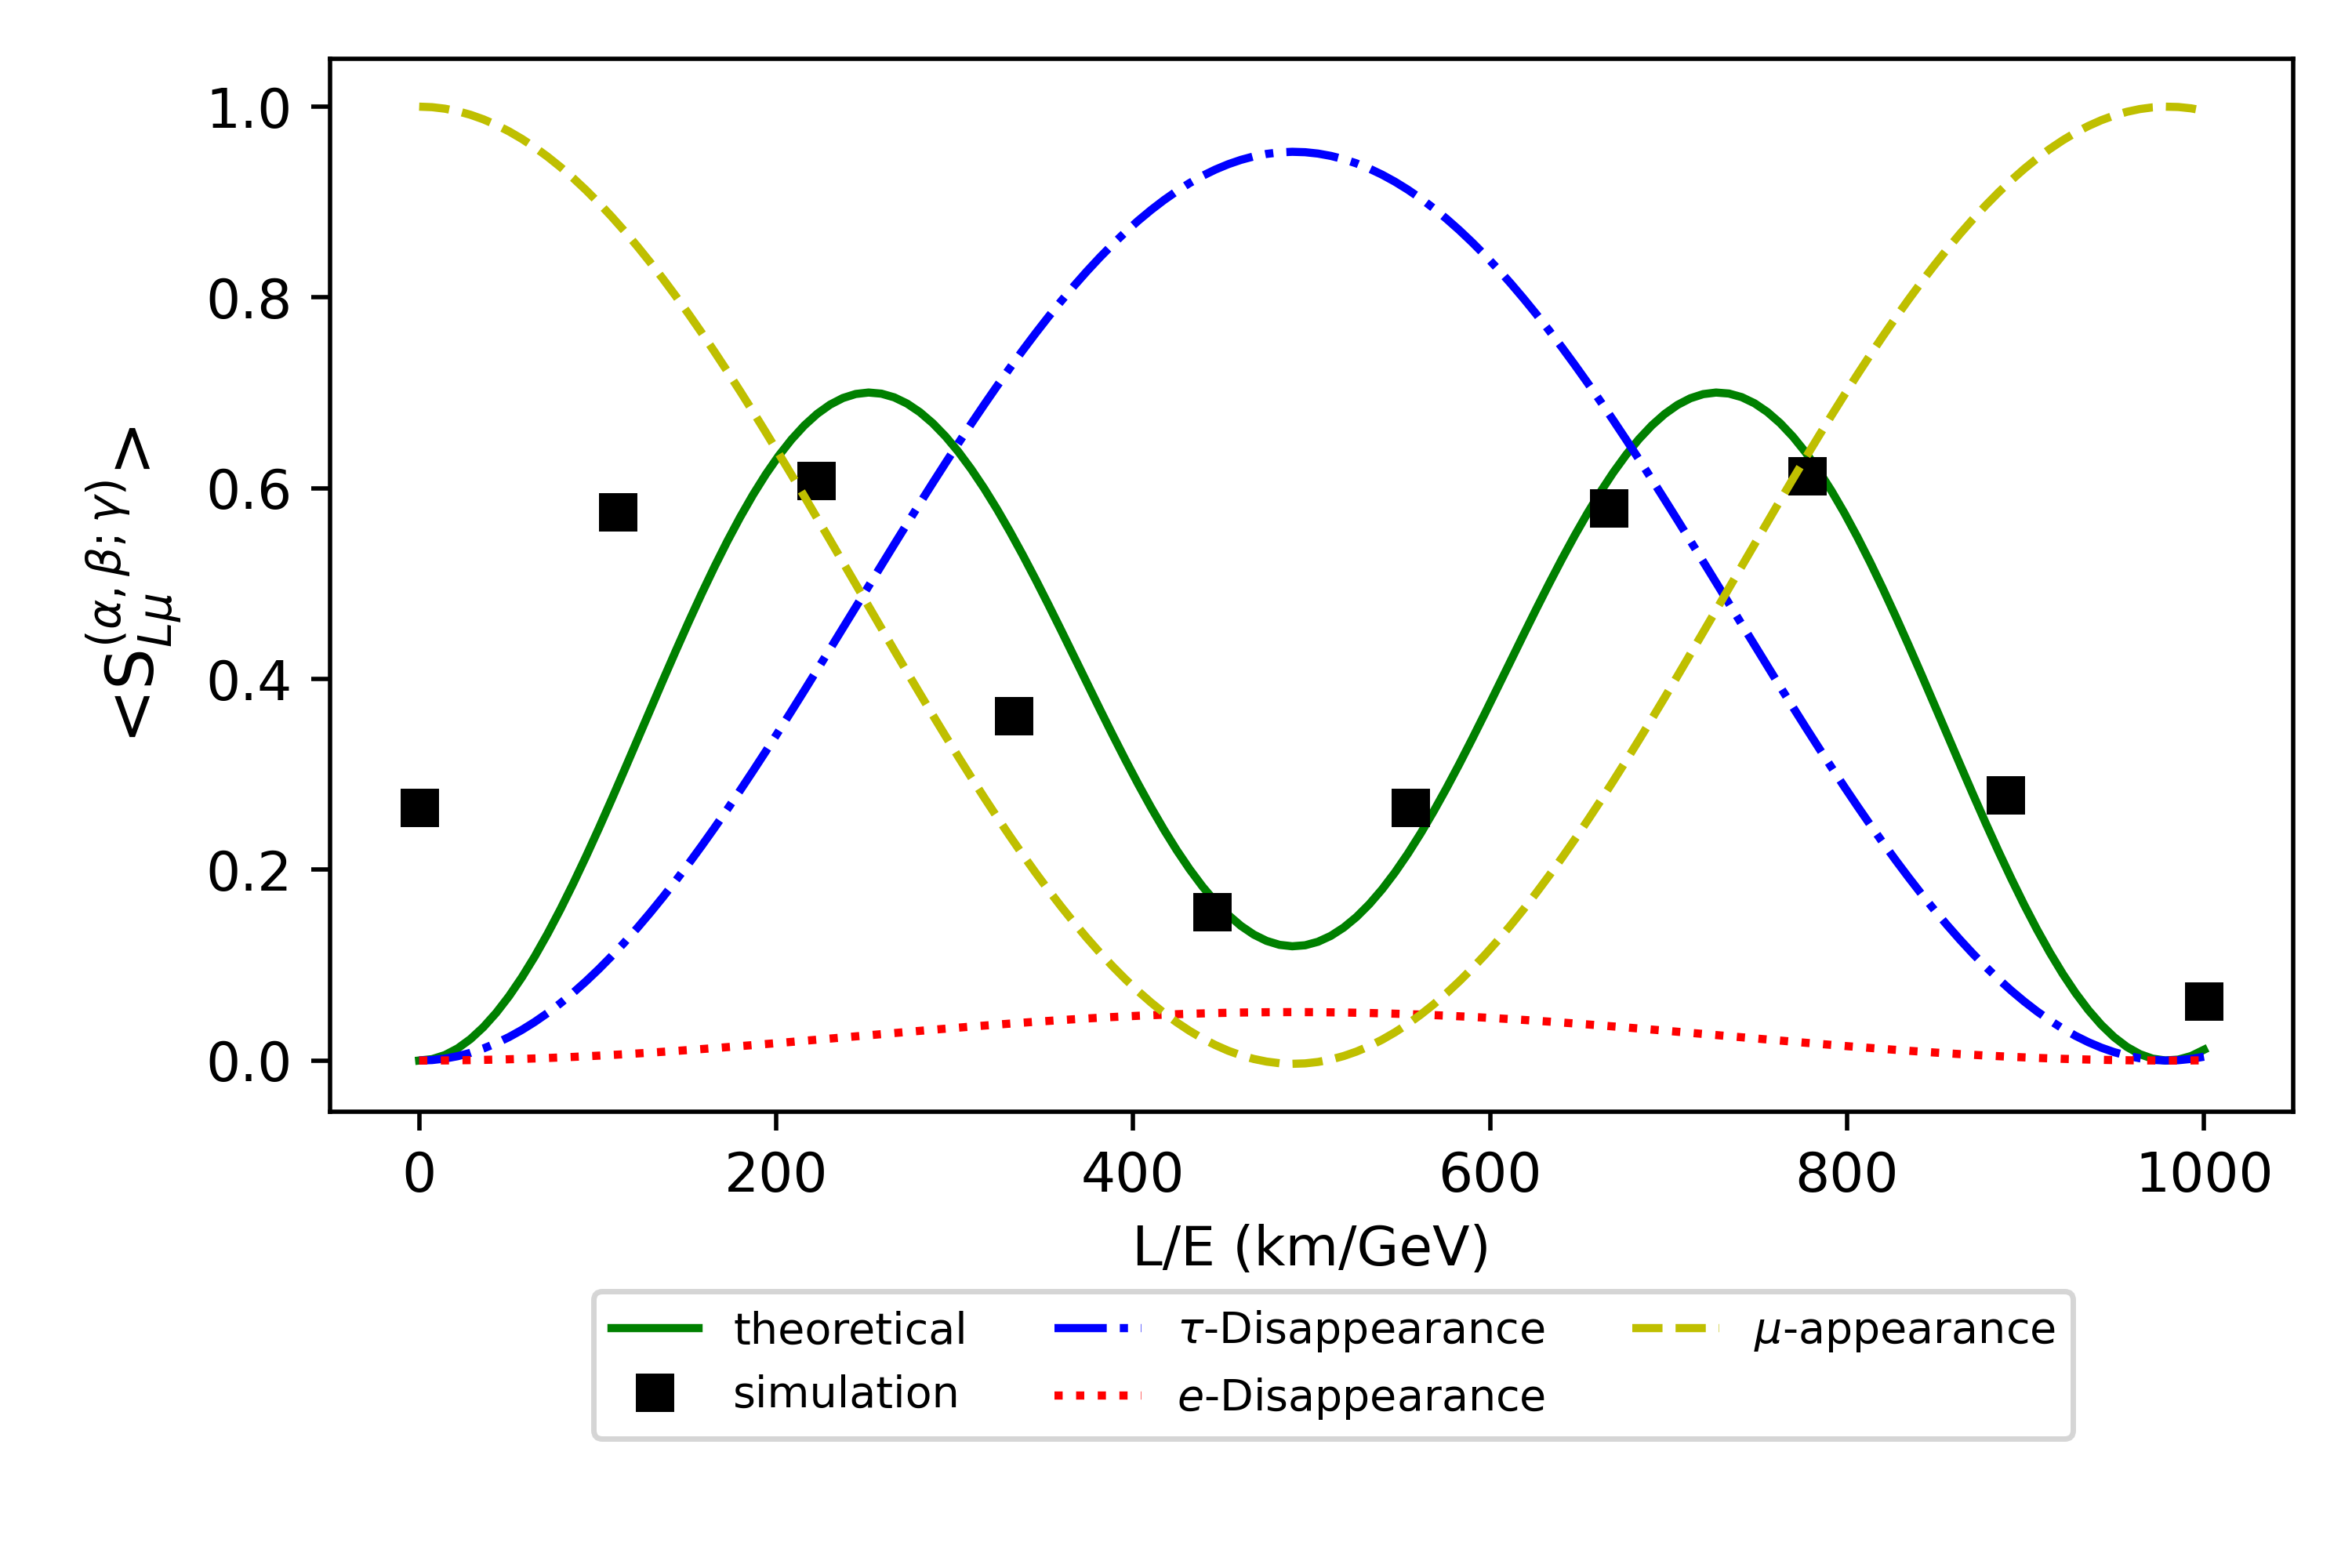
\includegraphics[width=0.8\textwidth]{fig_9a_2.png}}
	\caption{Global entanglement in the 3-flavour system (in Quantum computer).}
	\label{fig 9a_2}
\end{figure}
\pagebreak
Here $\langle S^{(\alpha,\beta;\gamma)}_{L\mu}\rangle$= Average linear entropy of the system. Average linear entropy is found out by considering all possible bi-partitions of the system. It is plotted as functiom of $\frac{L}{E}$. At constant value of $E$, average entropy solely depends upon $L$. In natural units $L=t$. Thus, at $t=0$ disappearance probability of muon is maximum. As a result, the average linear entropy of the system of the system will be zero. So that the flavour state at $t=0$ is not entangled (product state). Now as time progresses flavour oscillation happens and as result average linear entropy will vary. The global entanglement will be maximum when all oscillation probabilities (appearance and disappearance) are maximized.  
\newpage
\thispagestyle{empty}
\mbox{}
\newpage
\chapter*{Conclusion and Overview}
\addcontentsline{toc}{chapter}{\numberline{}Conclusion and Overview}
In this work, we conducted a brief review of quantum simulations. We intended to understand how quantum simulations of quantum systems were performed. Through our studies, we came to know that there are three kinds of quantum simulations; analog quantum simulations, digital quantum simulations and a hybrid of quantum-classical simulations. All of them slightly different from one another on aspects of how they encode the system, how they time evolve it and measure it. We were interested in digital quantum simulations. Digital quantum simulations are performed with the aid of a quantum computer. We used the quantum computing service provided by IBM Quantum to carry out the simulations. The problem we choose to study was the simulation of neutrino oscillation. We used the quantum algorithm or quantum circuit put forward by Arg\"uelles and Jones (2019) to carry out our study. \par
It is known for more than half a century that neutrino flavours exhibit oscillating behaviour analogous to kaon oscillations. While studying neutrino oscillation theory, we understood that it arises due to the non-coincidence of flavour and mass states of neutrino. In the ultra-relativistic limits, mass and flavour states are connected through the PMNS matrix. As a consequence, neutrinos oscillate between flavour states in a periodic fashion as time evolves. Under suitable approximation, neutrino oscillation would depend upon only five experimentally determined parameters ($\Delta m_{12}^{2},\Delta m_{13}^{2},\theta_{12},\theta_{23},\theta_{31}$).\par
To simulate neutrino oscillation, we encoded flavour states into qubits. The PMNS matrix required to transform between mass and flavour basis was constructed using quantum gates. In the two flavour case, the PMNS matrix could be easily constructed from a single qubit gate. While translating the problem to three flavour case, realising the PMNS matrix is non-trivial. The time evolution of neutrino states was simulated by apply unitary quantum gates to the qubits. Thus using a quantum circuit, we mimicked the time evolution of a neutrino flavour state. We study how the probabilities of each flavour vary as a function of both energies of the beam (E) and baseline (L). We performed simulations on both the QASM simulator and quantum computer. Results derived via simulations were matching with that of theoretical predictions.
Further, we conducted studies on the entanglement dynamics of the neutrino particle. Neutrinos were known to exhibit single-particle entanglement. Thus their flavour modes are in an entangled state. The amount of entanglement in the system can be measured using the linear entropy of the system. Linear entropy of the system takes a value between zero and one. The value of linear entropy is a direct indication of the amount of entanglement.  At the time when a neutrino is created, linear entropy is small. Thus the system will be minimally entangled. As time progress, neutrino oscillation happens, and the linear entropy of the system varies in a periodic manner. The system will maximally be entangled when the probability of appearance of all flavours together maximised.  We use the same circuit put forward by Arg\"uelles and Jones (2019) to evaluate this behaviour.  We verified these results in both the QASM simulator and quantum computer.\par
While performing simulation, excellent agreement theoretical predictions were obtained in the QASM simulator, especially in the two cases. However, often the values predicated by quantum computer varied from the theoretical predictions. The errors arise because quantum computers are not fault-tolerant. Quantum computers now available are prone to decoherence. Decoherence would influence the final result from the quantum computer. Also, it is known that error increases as a function of the length of the quantum circuit. We tried to understand the error in our simulation. While inspecting the residual plot, it is evident that errors not appear random. However, the exact reason occurrence of the error is still unknown to us. Nevertheless, one can mitigate the errors in the results by employing quantum error correction methods.

\begin{figure}[h]
	\graphicspath{ {./Images/} }
	\centering	
	{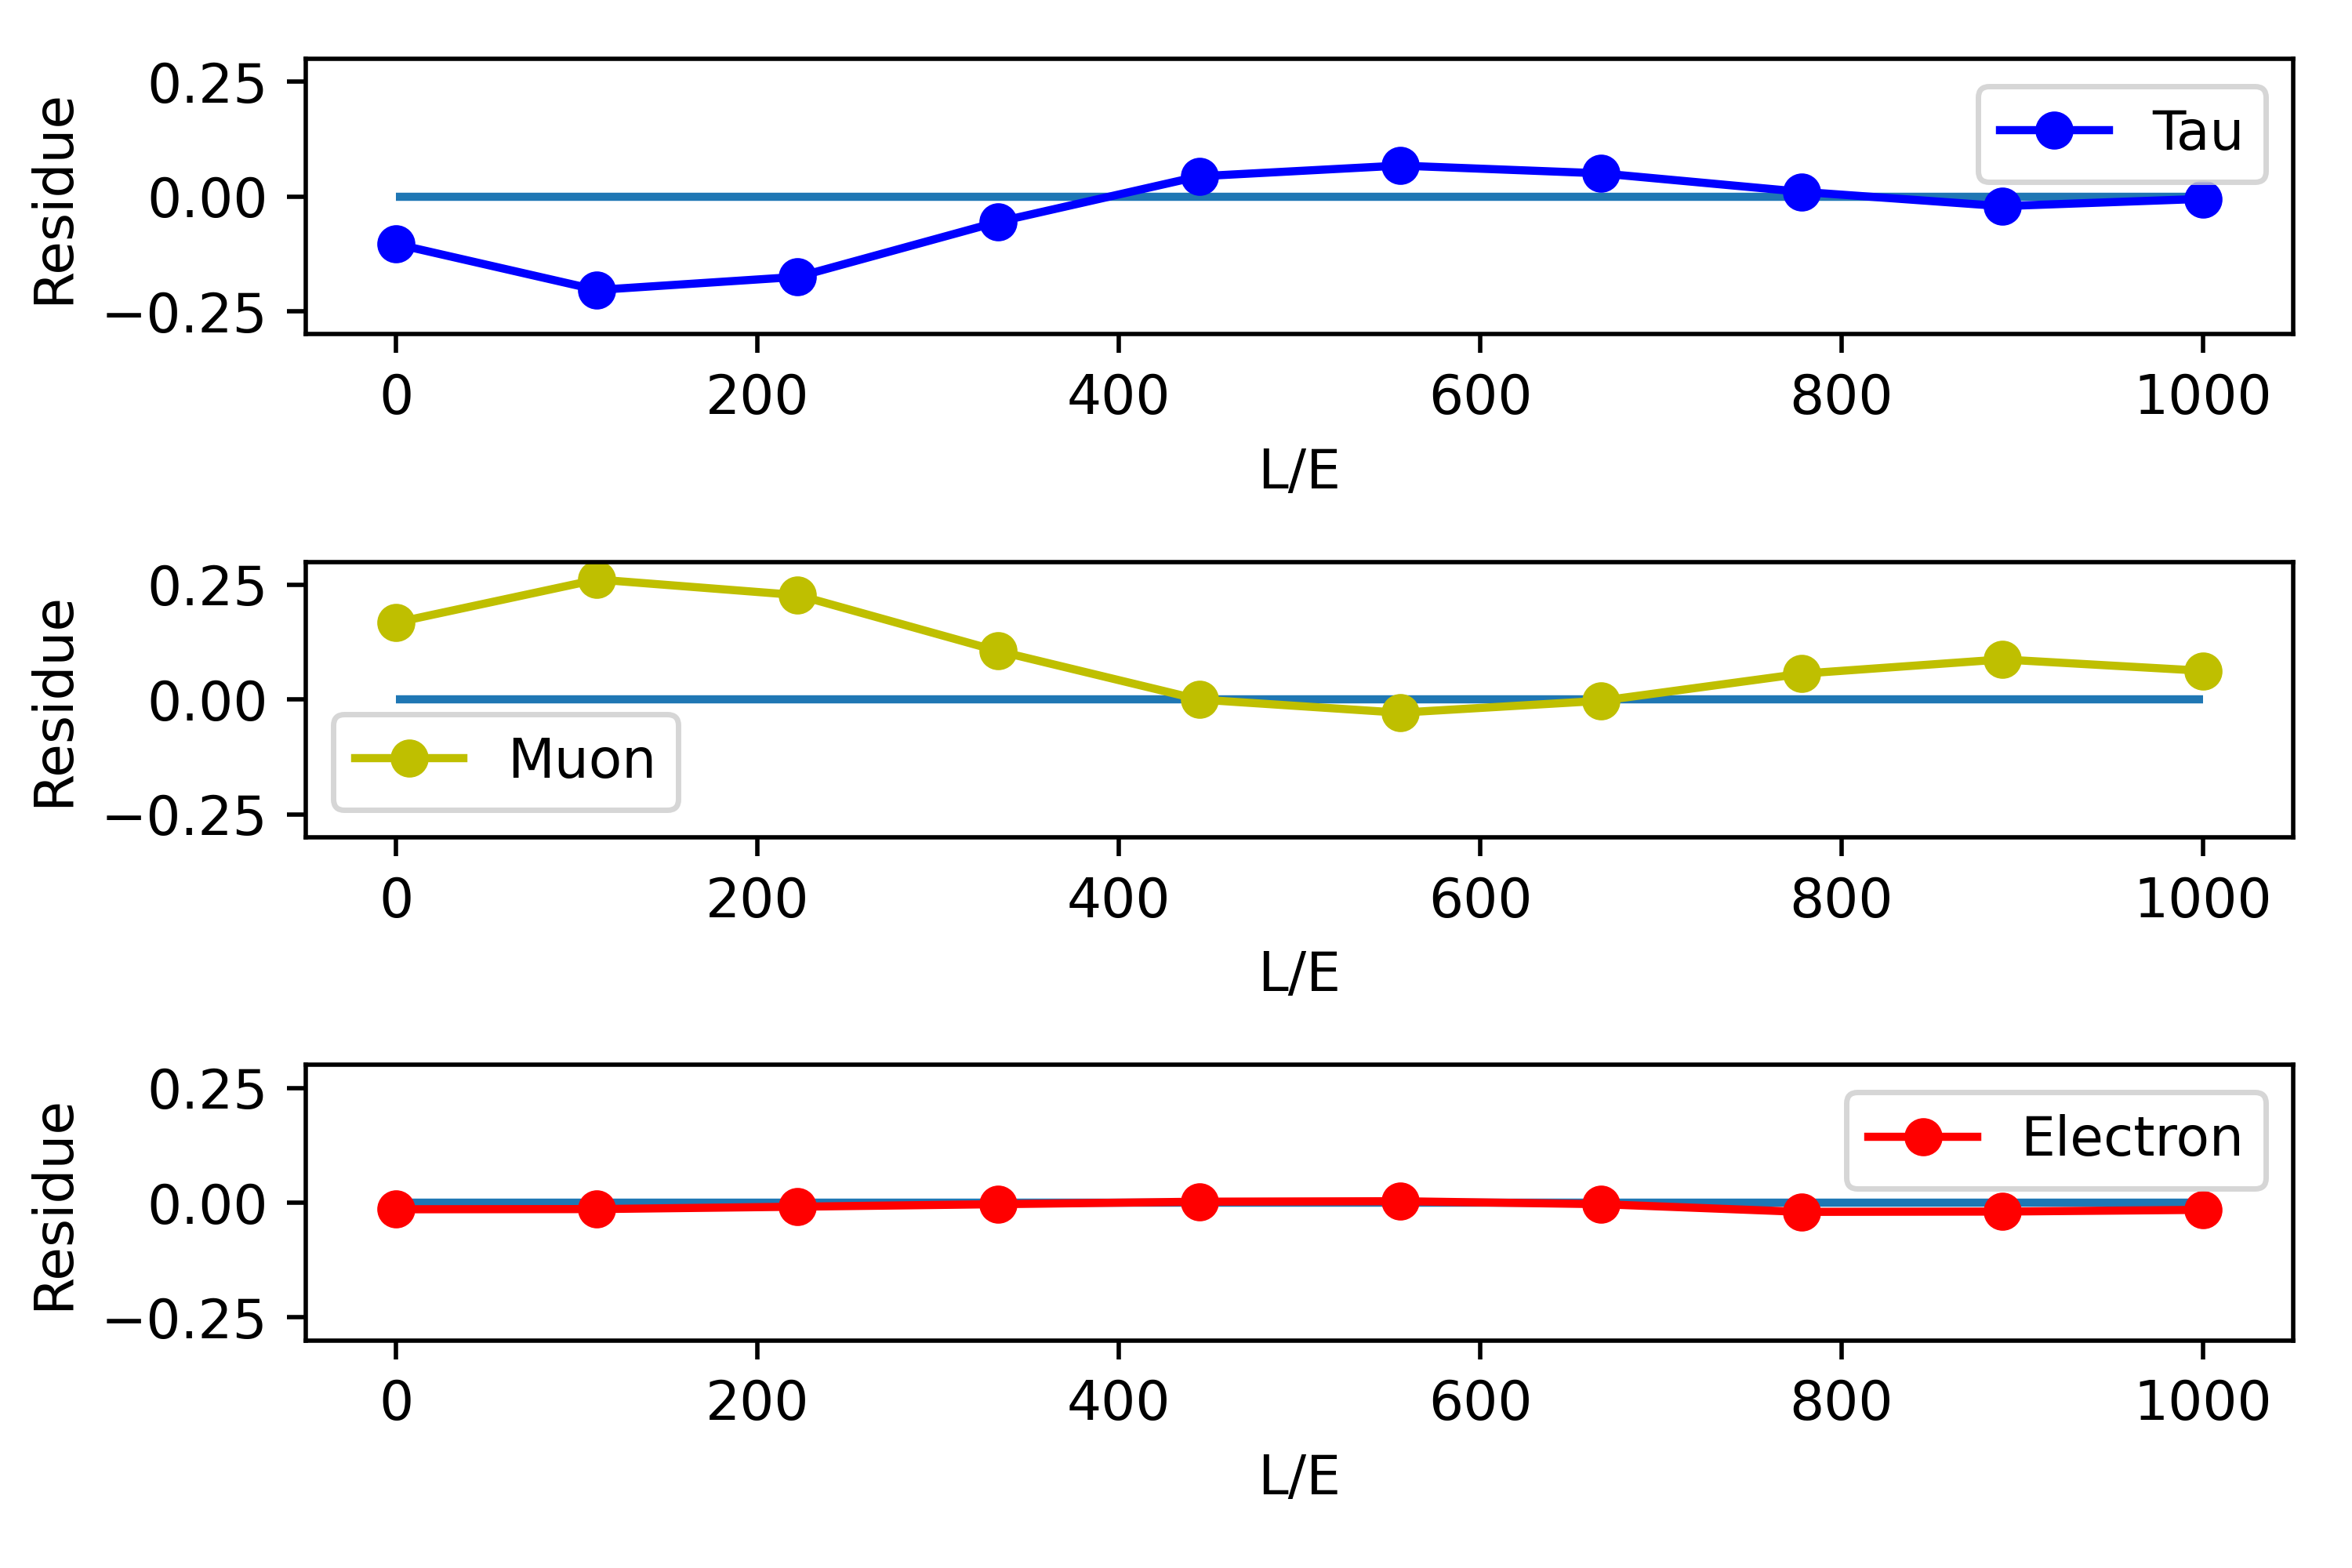
\includegraphics[width=0.8\textwidth]{fig_11.png}}
	\caption{Residue plot in the three flavour case}
	\label{fig 11}
\end{figure}
On analysing the results we got, one may become sceptical about the quantum advantage. The quantum advantage that was discussed earlier is not visible in our work. However, we were not intended to show the advantage of quantum simulation over the classical one. Our aim was to study the methodology of performing a simulation of a quantum system on a quantum computer. One can consider these works as baby steps towards the future where efficient quantum algorithms that surpass their classical counterparts exist.

\section*{Scope For Further Studies}
\begin{itemize}
	\item In our study, we studied neutrino oscillation in the ultra-relativistic approach. We assumed plane wave solutions for mass eigenstates while developing a theory of neutrino oscillation. There is another approach where wave packet solution is taken. Such an approach is instrumental in describing collective neutrino oscillations that happen near supernovae. One can work on simulating collective neutrino oscillation on quantum computers. A good starting point for those who interested will be \cite{hall}\cite{kubra}.
	\item In our work, matter effects in neutrino oscillation are left unstudied. By some modifications of the circuit, we can incorporate those effects in the simulation. Modifications to incorporate these effects is briefly discussed in \cite{jones}.
	\item From the residue plot, it is clear that error occurs during simulations appears to be not random. The reason for the occurrence of such a type of error is not addressed in our work. However,those who interested can look for the reasons for such errors. Also, one can look for error-correcting methods to mitigate the errors in our results.
	\item In addition to the entanglement shown by flavour states, mass states are also entangled. They show static entanglement. That is, entanglement measures do not vary with time. One can further investigate this topic and perform a quantum simulation to verify the results.

\end{itemize}
\vspace*{3cm}
\begin{center}
\noindent\rule{10cm}{0.4pt}
\end{center}

\bibliographystyle{unsrt}
\bibliography{ref}
\printindex

\end{document}


